\documentclass[12pt, a4paper, oneside]{report}

% for drawing trees 
\usepackage[linguistics, external]{forest}
\forestset{sn edges/.style={for tree={parent anchor=south, child anchor=north, s sep=10mm, inner sep=0mm}}}
 
\usepackage{tikz}
\usepackage{tikz-qtree}
\tikzset{every tree node/.style={align=center, anchor=north}}
\usetikzlibrary{positioning}

% externalizing figures, helps with compiling
\usetikzlibrary{external}
\tikzexternalize[prefix=tikzz/]


\usepackage{furkanframe}

\newcommand{\authname}{Furkan Atmaca} 
\newcommand{\ttitle}{Suspended Affixation in Turkish}
\newcommand{\ttitletr}{Türkçede Ertelenmiş Ekler}
\newcommand{\univname}{Boğaziçi University}
\newcommand{\degname}{Master of Arts}
\newcommand{\deptname}{Linguistics}
\newcommand{\supname}{Prof. Aslı Göksel}
\newcommand{\juryfname}{Assist. Prof. Pavel Logačev}
\newcommand{\jurysname}{Assist. Prof. Aslı Gürer}

%repeat the same in capitals
\newcommand{\authnamecaps}{FURKAN ATMACA} 
\newcommand{\ttitlecaps}{SUSPENDED AFFIXATION IN TURKISH}
\newcommand{\ttitletrcaps}{TÜRKÇEDE ERTELENMİŞ EKLER}
\newcommand{\univnamecaps}{BOĞAZİÇİ UNIVERSITY}
\newcommand{\degnamecaps}{MASTER OF ARTS}
\newcommand{\deptnamecaps}{LINGUISTICS}

\begin{document}

% frontmatter

\pagenumbering{gobble}
% cover page
${}$

\vspace{80pt}

\begin{center}
  \ttitlecaps
\end{center}

\vspace{150pt}

\begin{center}
	\authnamecaps
\end{center}

\vspace{150pt}

\begin{center}
	{\univnamecaps}
\\
  \the\year
\end{center}

\vspace{80pt}
${}$
\newpage
% title page
${}$
\vspace{55pt}


\begin{center}
  \ttitlecaps
\end{center}

\vspace{50pt}

\begin{center}
	Thesis submitted to the\\
	Institute for Graduate Studies in Social Sciences\\
	in partial fulfillment of the requirements for the degree of\\
\end{center}

\vspace{30pt}

\begin{center}
	\degname\\
	in\\
	\deptname
\end{center}

\vspace{30pt}

\begin{center}
	by\\
	\authname
\end{center}

\vspace{30pt}

\begin{center}
  \univname\\
  \the\year
\end{center}

\newpage

\vspace*{3cm}
\begin{center}
  \ttitle
\end{center}

\vspace{2cm}

\begin{center}
  The thesis of \authname\\
  has been approved by:
\end{center}

\vspace*{3cm}

\begingroup
\renewcommand{\arraystretch}{0.5}

\noindent
\begin{tabular}{p{0.5\textwidth}p{0.5\textwidth}}
  \supname & \makebox[5cm]{\hrulefill}\\
  (Thesis Advisor)&\\
  \vspace*{2em}&\\
  \juryfname & \makebox[5cm]{\hrulefill}\\ ${}$
  \vspace*{2em}&\\
  \jurysname & \makebox[5cm]{\hrulefill}\\
  (External Member)&\\
\end{tabular}

\endgroup

\vspace*{4cm}


\begin{center}
	\monthname\ \the\year
\end{center}


\chapter*{Declaration of Originality}

\vspace*{20pt}

\noindent I, \authname, certify that 
\begin{itemize} 
	\item I am the sole author of this thesis and that I have fully acknowledged and documented in my thesis all sources of ideas and words, including digital resources, which have been produced or published by another person or institution;
	\item this thesis contains no material that has been submitted or accepted for a degree or diploma in any other educational institution;
	\item this is a true copy of the thesis approved by my advisor and thesis committee at \univname, including final revisions required by them.
\end{itemize}
 
\vspace{40pt}

\noindent Signature:\\
\rule[0.5em]{25em}{0.5pt} % This prints a line for the signature
 
\noindent Date:\\
\rule[0.5em]{25em}{0.5pt} % This prints a line to write the date



\pagenumbering{roman}
\setcounter{page}{4}

\chapter*{Abstract\\ \ttitle}

"Lorem ipsum dolor sit amet, consectetur adipiscing elit, sed do eiusmod tempor incididunt ut labore et dolore magna aliqua. Ut enim ad minim
veniam, quis nostrud exercitation ullamco laboris nisi ut aliquip ex ea commodo consequat. Duis aute irure dolor in reprehenderit in
voluptate velit esse cillum dolore eu fugiat nulla pariatur. Excepteur sint occaecat cupidatat non proident, sunt in culpa qui officia
deserunt mollit anim id est laborum."


\newpage

\chapter*{Özet\\ \ttitletr}

"Lorem ipsum dolor sit amet, consectetur adipiscing elit, sed do eiusmod tempor incididunt ut labore et dolore magna aliqua. Ut enim ad minim
veniam, quis nostrud exercitation ullamco laboris nisi ut aliquip ex ea commodo consequat. Duis aute irure dolor in reprehenderit in
voluptate velit esse cillum dolore eu fugiat nulla pariatur. Excepteur sint occaecat cupidatat non proident, sunt in culpa qui officia
deserunt mollit anim id est laborum."


% moved renew commands for some ToC settings out of sty to here
\renewcommand\contentsname{TABLE OF CONTENTS}
\renewcommand\listfigurename{LIST OF FIGURES}
\renewcommand\listtablename{LIST OF TABLES}


\tableofcontents
\begingroup
\renewcommand{\addvspace}[1]{}
\printglossary[title=\MakeUppercase{abbreviations}, style=block,nonumberlist]
\listoftables
\listoffigures
\endgroup
\clearpage


% main body

\pagenumbering{arabic} 
\chapter{\MakeUppercase{introduction}}
% to reset the gb4e example count for each chapter
\setcounter{exx}{0}

\section{SA in Turkish} \label{whatisSA}
\section{Suspended affixation in Turkish} \label{whatisSA}

Suspended affixation is a morphological phenomenon where only one of the conjuncts has overt affixes that the other conjuncts share in interpretation. (\ref{suspended}) shows an abstract representation where there are two conjuncts `A' and `B' and the overt suffix(es) $\alpha$ on the second conjunct. SA is possible with more than two conjuncts (\ref{suspended2}).
\begin{exe}
\ex \begin{xlist}
\ex \label{suspended} A conjoiner B-$\alpha$
\glt Interpretation: `A-$\alpha$ conjoiner B-$\alpha$'

\ex \label{suspended2} A conjoiner B conjoiner C-$\alpha$
\glt Interpretation: `A-$\alpha$ conjoiner B-$\alpha$ conjoiner C-$\alpha$ '
\end{xlist}
\end{exe}

SA appears in languages usually as a backwards process, where the linearly rightmost conjunct bears the overt morphemes. Limited examples from Caucasian languages can also be found where affixes that occupy the left edge of the word are shared. (\ref{suspendreverse}) shows an example for SA of {\Fsg-\All} where the leftmost conjunct bears the overt suffix.
\begin{exe}
\ex \label{suspendreverse}
    \begin{xlist}
        \ex $\alpha-$A conjoiner B
        \glt Interpretation: `$\alpha-$A conjoiner $\alpha-$B'
        
        \ex Adyghe (Northwestern Caucasian) SA of {\Fsg-\All} \\*
        \gll s-j\textschwa-p\textctc a\textctc e-re \textteshlig'ale-re zezaox
        \\ {\Fsg}-{\All}-girl-{\And} boy-{\And} fight.each.other \\
        \glt `My son and daughter are fighting.'\\*
        \hfill Adapted from \cite{erschler2012suspended}
    \end{xlist}
\end{exe}

In the following paragraphs, I lay out the examples and configurations of Turkish SA in two parts. First is the nominal domain and the second is the verbal domain. Most examples of SA in the nominal domain are made with the {\Case}, {\Poss}, and {\Pl} suffixes in Turkish. Table \ref{tab:nominalSA} shows the suspendable suffixes in the nominal domain.

\begin{table}[hbt!]
    \caption{Suspendable Turkish Suffixes in Nominals}
    \centering
    \begin{tabular}{|ll|lllll}
    \hline 
        \multicolumn{2}{|c|}{Case} & \multicolumn{4}{|c|}{Possessive} & \multicolumn{1}{c|}{Plural} \\ \hline
        {\Acc} & \textit{-(y)I} &  \multicolumn{1}{l}{${}$} & 1$^{st}$ & 2$^{nd}$ & \multicolumn{1}{l|}{{\Third}$^{rd}$} & \multicolumn{1}{l|}{\textit{-lAr}} \\ \hline 
        
        {\Dat} & \textit{-(y)A} & {\Sg} & \textit{-(I)m} & \textit{-(I)n} &  \multicolumn{1}{l|}{\textit{-(s)I}} & ${}$ \\ \cline{1-6} 
        
        {\Loc} & \textit{-DA} & {\Pl} & \textit{-(I)mIz} & \textit{-(I)nIz} &  \multicolumn{1}{l|}{\textit{-lArI}} & ${}$ \\ \cline{1-6}
        
        {\Abl} & \textit{-DAn} & ${}$ & ${}$ & ${}$ & ${}$ & ${}$ \\ \cline{1-2}
        
        {\Gen} & \textit{-(n)In} & ${}$ & ${}$ & ${}$ & ${}$ & ${}$ \\ \cline{1-2}
    \end{tabular}
    \label{tab:nominalSA}
\end{table}

All the suffixes in Table \ref{tab:nominalSA} can be interpreted as $\varphi$-features\footnote{see \cite{harbour2008phi} and \cite{rezac2010phi} for the development and evaluations of $\varphi$ features.} and thereby inflectional, but some claim that derivational suffixes can also be suspended. That is going to be addressed in the following sections. In (\ref{nomex}), I give some possible examples of SA in the nominal domain.

\begin{exe}
    \ex \label{nomex} 
    \begin{xlist}
        \ex SA of {\Abl}\\*
        \gll Hoca ve ders-ten kork-uyor-um. \\
        instructor {\And} course-{\Abl} scared\_of-{\Prog}-{\Fsg} \\
        \glt `I fear the instructor and the course.'
        
        \ex SA of {\Poss-\Abl}\\*
        \gll Hoca ve ders-im-den kork-uyor-um. \\
        instructor {\And} course-{\Poss}.{\Fsg}-{\Abl} scared\_of-{\Prog}-{\Fsg} \\
        \glt `I fear my instructor and my course.' 
        
        \ex SA of {\Pl-\Poss-\Abl}\\*
        \gll Hoca ve ders-ler-im-den kork-uyor-um. \\ 
        instructor {\And} course-{\Pl}-{\Poss}.{\Fsg}-{\Abl} scared\_of-{\Prog}-{\Fsg} \\
        \glt `I fear my instructors and my courses.'
    \end{xlist}
\end{exe}
The sentences in (\ref{nomex}) show examples of full SA in a string of {\Pl}-{\Poss}-{\Case} in the first conjunct. Performing SA for all the suspendable suffixes is not obligatory, only {\Case} in a string of {\Pl}-{\Poss}-{\Case} can also be suspended. (\ref{nomex2}) illustrates this point.

\begin{exe}
    \ex \label{nomex2} SA of {\Abl} in a string of {\Pl-\Poss-\Abl}\\*
    \gll
    \textit{Hoca-lar-ım} ve ders-ler-im-den kork-uyor-um. \\ instructor-{\Pl}-{\Poss}.{\Fsg} {\And} course-{\Pl}-{\Poss}.{\Fsg} scared\_of-{\Prog}-{\Fsg} \\
    \glt `I fear my instructors and my courses.'
\end{exe}
The sentence in (\ref{nomex2}) shows the suspension of only {\Case} in the first conjunct in a string of {\Pl}-{\Poss}-{\Case}. Some deem an SA of {\Poss} ungrammatical in the example (\ref{nomex3}) where there is a suspension of {\Poss}-{\Case} in a string of {\Pl}-{\Poss}-{\Case}.

\begin{exe}
    \ex \label{nomex3}
    \gll 
    Hoca-lar ve ders-ler-im-den kork-uyor-um. \\ instructor-{\Pl} {\And} course-{\Pl}-{\Poss}.{\Fsg} scared\_of-{\Prog}-{\Fsg} \\
    \glt `?I fear my instructors and my courses.'
\end{exe}

SA is not exclusive to the conjunctions formed by \textit{ve} `ve', it can also take place in a conjunction formed by a negator like \textit{değil} `not', as shown in (\ref{nomex}).

\begin{exe}
    \ex \label{nomex4}
    \begin{xlist}
        \ex SA of {\Pl-\Abl}\\*
        \gll Ders değil hoca-lar-dan kork-uyor-um. \\ 
        course {\Neg} instructor-{\Pl}-{\Abl} scared\_of-{\Prog}-{\Fsg} \\
        \glt ${}$

        \ex SA of {\Abl}\\*
        \gll Ders-ler değil hoca-lar-dan kork-uyor-um. \\ 
        course-{\Pl} {\Neg} instructor-{\Pl}-{\Abl} scared\_of-{\Prog}-{\Fsg} \\
        \glt `I am not scared of the courses but the instructors.'
    \end{xlist}
\end{exe}

SA in the verbal domain has two shapes. One is the SA of agreement markers after TAM I markers. The other is the SA of TAM II and agreement markers together. I provide a list for inflectional suffixes in the verbal domain in Table \ref{tab:markers}. I give some possible examples for SA in the verbal domain in (\ref{verbex}).

\begin{table}[hbt!]
    \caption{TAM I, II, and Agreement Markers}
    \centering
    \begin{tabular}{|ll|lllll}
    \hline 
         \multicolumn{2}{|c|}{TAM I} & \multicolumn{2}{c|}{TAM II} &  \multicolumn{3}{c|}{Agreement} \\ \hline
        Aorist & \textit{-Ir} & Conditional & \textit{-(y)sA} & \multicolumn{1}{|l}{${}$} & \multicolumn{1}{c}{{\Sg}} & \multicolumn{1}{c|}{{\Pl}} \\ \hline
        
        Conditional & \textit{-sA} & Evidential & \textit{-(y)mIş} & \multicolumn{1}{|l}{1$^{st}$} & \textit{-(I)m} & \multicolumn{1}{l|}{\textit{-k}, or \textit{-(I)z}} \\ \cline{1-7}

        Future & \textit{-(y)AcAK} & Past & \textit{-(y)DI} & \multicolumn{1}{|l}{2$^{nd}$} & \textit{-(sI)n} & \multicolumn{1}{l|}{\textit{-(sI)nIz}} \\ \cline{1-7}
        
        Necessitive & \textit{-mAlI} & ${}$ & ${}$ & \multicolumn{1}{|l}{{\Third}$^{rd}$} & - & \multicolumn{1}{l|}{\textit{-lAr}} \\ \cline{1-2} \cline{5-7}
        
        Past & \textit{-DI} & ${}$ & ${}$ & ${}$ & ${}$ & ${}$ \\ \cline{1-2}
        
        Perfect/Evidential & \textit{-mIş} & ${}$ & ${}$ & ${}$ & ${}$ & ${}$\\ \cline{1-2}
        
        Progressive & \textit{-Iyor} & ${}$ & ${}$ & ${}$ & ${}$ & ${}$ \\ \cline{1-2}
    \end{tabular}
    \\
    ${}$ \hfill Adapted from \cite{goksel2001auxiliary}
    \label{tab:markers}
\end{table}

\begin{exe}
    \ex \label{verbex}
    \begin{xlist}
        \ex SA of {\Fsg}\\*
        \gll Ev-e gid-ecek ve dinlen-eceğ-im \\ 
        house-{\Dat} go-{\Fut} {\And} rest-{\Fut}-{\Fsg} \\
        \glt `I will go home and rest.'
        
        \ex SA of {\Evi-\Fsg}\\*
        \gll 
        Ev-e gid-ecek ve dinlen-ecek-miş-im. \\ 
        house-{\Dat} go-{\Fut} {\And} rest-{\Fut}-{\Cop}.{\Evi}-{\Fsg} \\
        \glt  `I was supposed to go home and rest.'
        
        \ex SA of {\Evi-\Fsg-\Prob}\\*
        \gll Ev-e gid-iyor ve dolan-ıyor-muş-um-dur. \\ 
        house-{\Dat} go-{\Fut} {\And} stroll-{\Prog}-{\Cop}.{\Evi}-{\Fsg}-{\Prob} \\
        \glt `I might have been going home and strolling.'
    \end{xlist}
\end{exe}

The sentences in (\ref{verbex}) show the suspension of only Agreement(\Fsg), suspension of TAM II and Agreement (\Evi-\Fsg), and suspension of TAM II, Agreement, and Probability marker \textit{-DIr} (\Evi-\Fsg-\Prob). The important observation made by the given examples is that SA is a rightward-bound process, meaning that the suspension of only $\alpha$ in a string of $\alpha-\beta$ is not allowed. It is either suspension of $\beta$, or $\alpha$-$\beta$.

Additionally, there are two configurations: one in compounding, and one in serial verb constructions in Turkish that could be considered as SA. The example in (\ref{compound-SA}) shows SA of compound/agreement marker ({\Poss}.{\Tsg} in glosses) on an inner compound. This marker is optionally covert in some cases. This optionality can be a suspension of the compound marker \textit{-(s)I(n)}.

\begin{exe}
    \ex \label{compound-SA}
    \gll Beykoz koru-(su) mesire alan-ı \\ 
    B grove-({\Poss}.{\Tsg}) picnic area-{\Poss}.{\Tsg} \\
    \glt `Beykoz grove's picnic area'
 \end{exe}
 
Another example of SA comes from serial verb constructions in Turkish. It is achieved with the suffix \textit{-(y)Ip} (Predicate Concatonator) {\Pc} in glosses). (\ref{ipSA}) shows an example of possible SA for the tense and agreement suffixes. Here the insertion of the suspended affixes is not allowed unlike the examples given so far.

\begin{exe}
    \ex \label{ipSA} SA of {\Pst-\Fsg}\\*
    \gll Ev-e gel-ip uyu-du-m. \\ 
    House-{\Dat} come-{\Pc} sleep-{{\Pst}}-{\Fsg} \\
    \glt `I came home and slept.'
\end{exe}

Suspendability of derivational suffixes show wide variation among suffixes and among native speakers. There are limited number of examples with varying degrees of acceptability\footnote{This is addressed more in depth in the first experiment I conducted in \S\ref{sec:testing}}. In (\ref{derivationalSA}), I give some possible examples of SA taking place with the derivational suffixes: \textit{-lI}, \textit{-sIz}, \textit{-lIK}, and \textit{-CI} ({\Der} in glosses). Remember that these examples are not widely acceptable and display great variation.

\begin{exe}
    \ex \label{derivationalSA}
    \begin{xlist}
        \ex SA of \textit{-lI}\\*
        \gll ?Çilek ve çikolata-lı dondurma \\ 
        strawberry {\And} chocolate-{\Der} ice\_cream \\
        \glt `Ice cream with chocolate and strawberry'
        
        \ex SA of \textit{-sIz}\\*
        \gll ?Şeker ve yağ-sız yiyecek-ler \\ 
        sugar {\And} fat-{\Der} food-{\Pl} \\
        \glt `Sugar and fat free foods'
        
        \ex SA of \textit{-lIK}\\*
        \gll ?Bahar ve yaz-lık ceket \\ 
        spring {\And} summer-{\Der} jacket \\
        \glt `Spring and summer jacket'
        
        \ex SA of \textit{-CI}\\*
        \gll ?futbol ve basket-çi \\ 
        football {\And} basketball-{\Der} \\ 
        \glt `Football and basketball player'
    \end{xlist}
\end{exe}


\section{Coordination}

\section{Ellipsis}

\section{Distributed Morphology}

\section{Lexical Functional Grammar}





\chapter{\MakeUppercase{Literature Survey}} \label{litsurvey}
% to reset the gb4e example count for each chapter


\cite{geoffrey1967turkish} is credited with the term SA and first observations of it in Turkish. Categorized as an agglutinating language with many inflectional and derivational functions represented by distinct morphemes, Turkish has many affixes that can be suspended, both in nominal and verbal domains. Some papers that exclusively examine SA in Turkish are: \cite{orgun1995flat}, \cite{kabak2007turkish}, \cite{broadwell2008turkish}, \cite{kornfilt2012revisiting}, \cite{kharytonava2012word,kharytonava2012taming}, and \cite{akkucs2016suspended}.

Some other papers investigating SA in other languages are: \cite{erschler2012suspended}, and \cite{erschler2018suspended} for Ossetic, \cite{yoon2017lexical} for Korean, \cite{despic2017suspended} for Serbian, \cite{guseva2017postsyntactic} for Mari, and \cite{pounder2006broken} for German. These papers range from giving the relative data and its limitations to the structural accounts and predictions for SA. In this chapter I first summarise the literature regarding SA in Turkish, later I summarise the literature regarding SA in other languages.


\section{Turkish}

\subsection{\cite{orgun1995flat}} \label{orgun}

Orgun argues for an analysis of SA as a structural sharing process. He provides the examples in (\ref{tebrikler}). These examples show that SA of {\Poss} is ungrammatical in a string of {\Pl-\Poss}. This is peculiar considering that in (\ref{possSA}), SA of {\Poss} is grammatical. 

\begin{exe}
    \ex \label{tebrikler}
    \begin{xlist}
    \ex SA of {\Poss} \label{tebriklerug}\\*
    \gll *tebrik-ler ve teşekkür-ler-im \\ 
    congrats-{\Pl} {\And} thanks-{\Pl}-{\Poss}.{\Fsg} \\
    \glt ${}$
    
    \ex SA of {\Pl-\Poss} \label{tebriklerg}\\*
    \gll tebrik ve teşekkür-ler-im \\ 
    congrats {\And} thanks-{\Pl}-{\Poss}.{\Fsg} \\
    \glt `My congratulations and thanks'
    \end{xlist}
    
    \ex \label{possSA}
    \begin{xlist}
        \ex SA of {\Poss}\\*
        \gll Kitap ve kalem-im \\
        book {\And} pencil-{\Poss}.{\Fsg} \\
        \glt `My book and my pencil'
    \end{xlist}
\end{exe}

Orgun proposes to place the suffixes {\Pl} and {\Poss} on the same hierarchical level as in Figure \ref{fig:orgun2}. This way, he explains the ungrammatical SA of {\Poss} (\ref{tebriklerug}) and grammatical SA of {\Poss} (\ref{possSA}). The string of {\Pl-\Poss} are interpreted as hierarchically equivalent so SA cannot target only one of them. 

\begin{figure}[hbt!]
    \centering
    \begin{forest}
        [N
            [N]
            [{\Pl}]
            [{\Poss}]]
    \end{forest}
    \caption{Ternary branching analysis for SA}
    \label{fig:orgun2}
\end{figure}

He provides a three-way ambiguity of an expression like \textit{it-ler-i} `dog-{\Pl}-{\Poss}' (\ref{itleri}) for the support of ternary branching (\ref{fig:orgun2}). The three-way ambiguity results from the order of composition. All items are on the same hierarchical level, so the order of composition becomes ambiguous resulting in the different readings.
\begin{exe}
    \ex \label{itleri}
    \gll \textit{it-ler-i} \\ dog-{\Pl}-{\Poss} \\
    \glt `her/his dogs' \\* `their dog' \\* `their dogs' \\*
    \hfill Adapted from \cite{orgun1995flat}
\end{exe}

Reading in between the lines, I assume that Orgun takes {\Pl} and {\Poss} suffixes to have a different interaction than any other pair of suffixes holds, in a way that they form a complex head when they are adjacent. What he is proposing is not a ternary branching but a complex head formation. A representation of this formulation reflected on the ungrammatical SA in (\ref{tebriklerug}) is given in Figure \ref{fig:furkan1}.

\begin{figure}[hbt!]
    \centering
    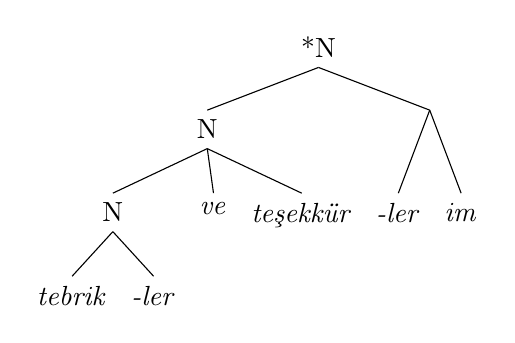
\begin{tikzpicture}
    \Tree[.*N
            [.N 
                [.N 
                    [.\textit{tebrik} ]
                    [.\textit{-ler} ] ]
                [.\textit{ve} ]
                [.\textit{teşekkür} ] ]    
            [ 
                [.\textit{-ler} ]
                [.\textit{im} ] ]
        ];
    \end{tikzpicture}
    \caption{{\Pl} and {\Poss} forming a complex head in ungrammatical SA}
    \label{fig:furkan1}
\end{figure}


Forming a complex head of {\Pl-\Poss} makes the interpretation of the word \textit{tebrikler} and the suffix \textit{ler-im} `{\Pl-\Poss}' ungrammatical. The same complex head, however, does not cause a problem for the grammatical SA in (\ref{tebriklerg}) as Figure \ref{fig:furkan2} shows. Figure \ref{fig:furkan2} has equivalent conjuncts and an interpretable relation between the complex suffix \textit{-ler-im} `{\Pl-\Poss}' and the nouns \textit{tebrik} `congrats', and \textit{teşekkür} `thanks'. 

\begin{figure}[hbt!]
    \centering
    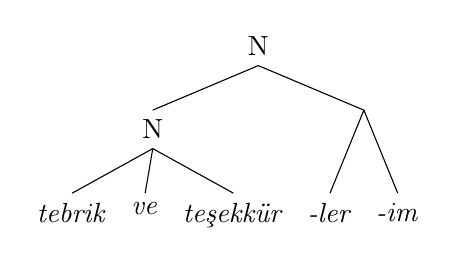
\begin{tikzpicture}
    \Tree[.N
            [.N 
                [.\textit{tebrik} ]
                [.\textit{ve} ]
                [.\textit{teşekkür} ] ]
            [ 
                [.\textit{-ler} ]
                [.\textit{-im} ] ]
    ];
    \end{tikzpicture}
    \caption{{\Pl} and {\Poss} forming a complex head in grammatical SA}
    \label{fig:furkan2}
\end{figure}




Orgun goes on to show that ternary branching is needed for some morphological configurations to satisfy the minimal phonological size ($\sigma\sigma$) constraint, citing \cite{ito1989notes}, together with \cite{orgun1992turkish}. He proposes a structural sharing analysis for SA and a ternary branching for {\Pl} and {\Poss} suffixes to capture the inseparable SA of {\Pl-\Poss}. Support for ternary branching in SA comes from somewhat unrelated phonological constraints in affixation of monosyllabic words, i.e. \textit{*do-m} [$\sigma$] `do-{\Poss}.{\Fsg}', \textit{sol-üm} [$\sigma$-$\sigma$] `sol-{\Poss}.{\Fsg}'. The ungrammatical SA in (\ref{tebrikler}) is not subject to such a constraint and the three-way ambiguity of an expression like \textit{it-ler-i} `dog-{\Pl}-{\Poss}' is not convincing enough to propose ternary branching. In finalizing the observation that Orgun makes, I provided Figures \ref{fig:furkan1} and \ref{fig:furkan2} following the discussion and the examples provided in \cite{orgun1995flat} to paint a more comprehensible picture of his analysis.


\subsection{\cite{kabak2007turkish}}
Among the papers discussing SA in Turkish, Kabak's paper seems to be the most extensive in terms of providing how SA can take shape in both verbal and nominal domains. The paper provides the conditions in which we can expect SA. The analysis of Kabak relies on the definition of a morphological word. Kabak claims that any inflectional morpheme can be suspended as long as the remainder is a morphological word. Kabak proposes the following:
\begin{itemize}
    \item Terminal suffix: \textit{A suffix that is allowed to appear at the end of a word, where further affixation is not obligatory.}
\end{itemize}
He claims that only terminal suffixes can be suspended. He posits that bare verbs are not morphological words in Turkish. He provides Table (\ref{tab:terminalmorphemes}) for Verbal terminal suffixes.
\begin{table}[hbt!]
\caption{Verbal Terminal Morphemes}
    \centering
    \begin{tabular}{|ll|}
    \hline 
                                    {(i) Agreement markers} &  \\ \hline
         \multirow{5}{20em}{(ii) Aspect/ Modality markers}  & {\Aor} \textit{-(I)r/(A)r} \\ 
                                                            & {\Prog} \textit{-Iyor} \\
                                                            & {\Fut} \textit{-(y)AcAK} \\
                                                            & {\Evi} \textit{-mIş} \\
                                                            & {\Nec} \textit{-mAlI} \\ \hline
        \multirow{2}{20em}{(iii) Converb markers}           & \textit{-(y)IncA} \\
                                                            & \textit{-(y)Ip} \\
    \hline                                                         
    \end{tabular}
    \label{tab:terminalmorphemes}
\begin{flushright}
    Adapted from \cite{kabak2007turkish}
\end{flushright}
\end{table}

If any suspension attempt is made with these morphemes, it is only permitted under the condition that what is left is a morphological word. Kabak classifies such clitics \textit{=mI}, and \textit{=DA} as non-terminal but also recognizes their ability to end an expression in Turkish (\ref{clitics}).

\begin{exe}
    \ex \label{clitics}
    \begin{xlist}
    \begin{multicols}{2}
        \ex
        \gll
        \textit{koş-tu-n} \textit{mu?} \\ run-{{\Pst}}-{\Second}{\Sg} =Q \\
        \glt `Did you run?'
        
        \ex 
        \gll
        \textit{ağla-mış-sın} \textit{da} \\ cry-{\Evi}-{\Second}{\Sg} =TOO \\ 
        \glt `It looks like you have cried also.'
    \end{multicols}
    \end{xlist}
    \hfill Adapted from \cite{kabak2007turkish}
\end{exe}
Kabak argues against \cite{kornfilt1996some}'s formulation for SA (\ref{kornfiltsa}) with two examples. According to \cite{kornfilt1996some}'s analysis only the copular forms and further inflectional morphemes can be suspended.
\begin{exe}
    \ex \label{kornfiltsa}
    [V$_{Participle}$ conjunction V$_{Participle}$] + V$_{Copula}$ + Inflectional Morphemes
\end{exe}

First, some forms that can be complements of copula are not participles and do not always give way to grammatical instances of SA. Although \cite{kornfilt1996some} does not define \textit{-DI} as a participle, it is still able to be a complement to a copular \textit{i}. Hence an expected SA in (\ref{kornfiltpart}) where the suspension is applied to the copula and not the participle.

\begin{exe}
    \ex \label{kornfiltpart}
    \begin{xlist}
        \ex
        \gll
        \textit{*O} \textit{yaz} \textit{Finike-ye} \textit{git-ti} \textit{ve} \textit{deniz-e} \textit{gir-di-y-di-k.} \\ that summer Finike-{\Dat} go-{{\Pst}} {\And} sea-{\Dat} enter-{{\Pst}}-{\Cop}-{{\Pst}}-{\First}.{\Pl} \\
        
        \ex 
        \gll 
        \textit{*Ev-im-iz-i} \textit{sat-sa} \textit{ve} \textit{bir} \textit{dükkan} \textit{al-sa-y-dı-k.} \\ house-1-{\Pl}-{\Acc}. sell-{\Cond}. {\And} a shop buy-{\Cond}.-{\Cop}-{{\Pst}}-{\First}.{\Pl} \\
    \end{xlist}
\hfill Adapted from \cite{kabak2007turkish}
\end{exe}

Second, at least one suffix deemed participle, namely the necessitative marker \textit{-mAlI}, does not behave like a participle that can modify NPs unlike other participles like \textit{-mIş} and \textit{-(y)AcAK} (\ref{kabakmali}). It should be noted however, contra Kabak, not all participle forms can modify nouns for example \textit{-Iyor}, and despite a lack of modifying capability, \textit{-mAlI} acts as predicted by \cite{kornfilt1996some}.
\begin{exe}
    \ex \label{kabakmali}
    \gll 
    \textit{*çalış-malı} \textit{adam} \\ work-{\Nec}. man \\
\end{exe}
% Kornfilt deems any inflection that is a complement of copula as participle, and Kabak points to this generalization being faulty in accurately predicting instances of SA in verbal domain.

Another point Kabak provides, contradicting Orgun, is the suspension of possessive when coming after a plural marker (\ref{plurposs}).

\begin{exe}
    \ex \label{plurposs}
    \gll
    \textit{Asker-ler} \textit{ve} \textit{komutan-lar-ım-ız.} \\ soldier-{\Pl} {\And} commander-{\Pl}-{\Poss}.{\First}-{\Pl} \\
    \glt `Our soldiers and commanders'
    \hfill Adapted from \cite{kabak2007turkish}
\end{exe}

Kabak provides an approach that is rather interesting. He makes an observation from \cite{good2005morphosyntax}, in the spirit of \cite{erdal2000clitics}, about the agreement paradigms in Turkish. In his citing, Kabak says that z-paradigm of agreement markers contain cliticized forms of words, and k-paradigm of agreement has lexical suffixes, thereby explaining the ungrammaticalities in (\ref{kornfiltpart}). Kabak also realizes the shortcomings of this approach and notes there are constructions in which k-paradigm SA is applicable and other conditions where z-paradigm SA is not applicable. As a last summary of Kabak's observations, he gives the following points in verbal domain SA:
\begin{exe}
\sn \begin{xlisti}
    \ex the ability of a verbal morpheme to terminate a word is related to its ability to stand without an agreement marker
    \ex SA is only applicable if what is left after suspension is a morphological word, and both the conjuncts end with terminal morphemes
    \ex Conjuncts with cliticlike endings are interpreted as 3$^{rd}$ person singular, causing agreement mismatches in SA
    \ex Nonfinal conjunct's terminal suffix must be overt
    \end{xlisti}
    \hfill Adapted from \cite{kabak2007turkish}
\end{exe}

Kabak recognizes that in SA what is relevant is actually the size of what is left after SA. Not on the lower end of the size, but also at the higher end. However the `cliticlike' condition on his third point is not clear-cut, and can be extended to other suffixes which have 3$^{rd}$ person singular suffixes which allow SA, which seemingly can end a word without copula. \textit{-mIş}, \textit{-(y)AcAK}, and \textit{-Iyor} to name a few. This condition relies heavily on what is `cliticlike' and gives way to wrong predictions in SA. His explanations are not based on a theoretical framework, which makes some of the explanations arbitrary. 

\subsection{\cite{broadwell2008turkish}}
Broadwell provides a representation for the SA using the tools of Lexical Functional Grammar (LFG henceforth). In this approach the two identical phrases form a new phrase in conjunction that has the same structural properties of its parts. After this point, the suspended affixes are added. The phonological exponent of the right edge conjunct and the suspended affixes are \textit{coinstantiated} as one word. A structural representation for (\ref{tebrikler3}) is given in Figure (\ref{fig:lexicalshare}).

\begin{exe}
    \ex \label{tebrikler3}
    \gll 
    tebrik ve teşekkür-ler-im \\ congrats and thanks-{\Pl}-{\First}.{\Sg} \\ 
    \glt `My congratulations and thanks'
\end{exe}
    
\begin{figure}[hbt!]
    \centering
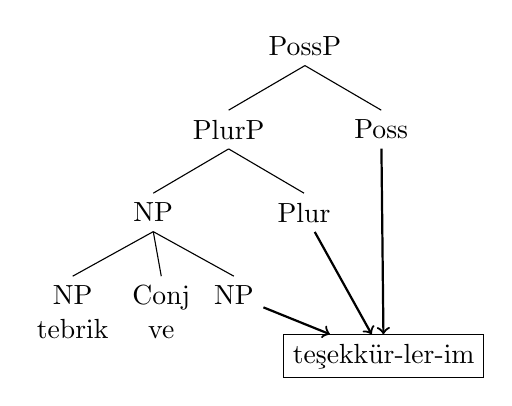
\begin{tikzpicture}
    \Tree[.PossP
            [.PlurP 
                [.NP 
                    [.NP\\tebrik ]
                    [.Conj\\ve ]
                    [.\node(NP2){NP}; ] ]
                [.\node(plr){Plur}; ] ]
            [.\node(PS){Poss}; ]
]
\node[below right= 1em of NP2, draw](co){teşekkür-ler-im};
\draw[thick, ->] (NP2) -- (co);
\draw[thick, ->] (plr) -- (co);
\draw[thick, ->] (PS) -- (co);
\end{tikzpicture}
    \caption{Lexical sharing analysis of {\Pl} and {\Poss} in SA}
    \label{fig:lexicalshare}
\end{figure}

Broadwell claims that this way of representation for SA saves us from three things:
\begin{itemize}
    \item  interpreting affixes that can suspend as clitics
    \item positing conjunction in the lexicon
    \item having special annotation for the rightmost conjunct
\end{itemize}
I will not go into the details of the alternatives for this analysis, but an important point which Broadwell makes is that Turkish is relatively productive in SA but it also makes distinctions that can not be addressed with a purely lexical approach. It might be posited that SA is only permitted with affixes that can attach to conjoined phrases. Then the question is why there are some morphemes that can happen to modify conjoined phrases but some others not, and how one makes a distinction between the two types.

\subsection{\cite{kornfilt2012revisiting}} \label{kornfilt}
Kornfilt reiterates points in \cite{kornfilt1996some}. Mainly that SA is a syntactic operation much like gapping or ellipsis, that can only target syntactic categories, and she gives her account of RNR (Right Node Raising) to account for SA. She claims that a suffix can be suspended only if it has a syntactic projection. In this way she predicts to posit functional heads like Num (NumP), Case (KP), and Possession (PossP) since all three can have SA distinctly. Figure \ref{fig:kornfilt} illustrates the abstract RNR analysis for the examples of SA in (\ref{heads}).
\begin{exe}
    \ex \label{heads}
    \begin{xlist}
        \ex \label{heads1} SA of {\Pl}\\*
        \gll Kitap ve defter-ler \\ 
        book {\And} notebook-{\Pl} \\
        \glt Reading1: `Books and notebooks' \\*
        Reading2: `A book and notebooks'
        
        \ex \label{heads2} SA of {\Acc}\\*
        \gll Kitap ve defter-i al-dı-m. \\ 
        book {\And} notebook-{\Acc} buy-{\Pst}-{\Fsg} \\
        \glt `I bought the book and the notebook.'
        
        \ex SA of {\Poss}\\*
        \gll Kitap ve defter-im nerede? \\ 
        book {\And} notebook-{\Poss}.{\Fsg} where \\
        \glt Reading1: `Where is the book and my notebook?' \\* 
        Reading2: `Where is my book and notebook?'
    \end{xlist}
\end{exe}


\begin{figure}[hbt!]
    \centering
    \begin{forest}
        [ConjP, s sep=30mm
            [Conj' 
                [XP$_1$ 
                    [YP]
                    [X$_1$, name=x1]]
                [Conj]
                [XP$_2$ 
                    [YP]
                    [X$_2$, name=x2]]]
            [X, name=x3]]
\draw[rounded corners=1em, ->] (x1.south) -- ++(south:2em) -| (x3.south);
\draw[rounded corners=1em, ->] (x2.south) -- ++(south:1em) -| (x3.south);
    \end{forest}
    \caption{RNR proposal for SA}
    \label{fig:kornfilt}
\end{figure}

This analysis is also the same analysis that Kornfilt provides for backwards ellipsis for a sentence like (\ref{backwardellipsis}) as in Figure \ref{fig:backwardellipsis}. This way Kornfilt regards SA as another ellipsis process operating on projection heads instead of phrases.

\begin{exe}
    \ex \label{backwardellipsis}
    \gll Ahmet al-dı ve Mehmet sat-tı kitab-ı. \\ 
    A[{\Nom}] buy-{\Pst}[{\Tsg}] {\And} M[{\Nom}] sell-{\Pst}[{\Tsg}] book-{\Acc} \\
    \glt `Ahmet bought and Mehmet sold the book.'
\end{exe}

\begin{figure}[hbt!]
    \centering
    \begin{forest}
        [ConjP, s sep=30mm 
            [Conj' 
                [TP 
                    [DP\\\textit{Ahmet}]
                    [\ldots 
                        [\sout{DP}, name=tk]
                        [V\\\textit{al}]]]
                [Conj\\\textit{ve}]
                [TP 
                    [DP\\\textit{Mehmet}]
                    [\ldots 
                        [\sout{DP}, name=tl]
                        [V\\\textit{sat}]]]]
            [DP\\\textit{kitab-ı}, name=DP]]
\draw[rounded corners=1em, ->] (tk.south) -- ++(south:2.5em) -| (DP.south);
\draw[rounded corners=1em, ->] (tl.south) -- ++(south:1.5em) -| (DP.south);
    \end{forest}
    \caption{RNR analysis for Backward Ellipsis}
    \label{fig:backwardellipsis}
\end{figure}

Kornfilt argues against SA of derivational suffixes because an example like (\ref{kornfiltder}) has a fixed order of conjuncts for a successful suspension. This makes a clear distinction for what is possible to suspend and what is not. 

\begin{exe}
    \ex \label{kornfiltder}
    \begin{xlist}
        \ex \gll [tuz ve limon]-luk \\ salt {\And} lemon-{\Der} \\ 
        \glt `[salt and lemon] shaker'
        
        \ex \gll *[limon ve tuz]-luk \\ lemon {\And} salt-{\Der} \\
        \glt `[lemon] and [saltshaker]'
    \end{xlist}
\end{exe}

The proposed analysis of Kornfilt does not explain why SA of {\Poss} is ungrammatical in a string of {\Pl-\Poss}. As a terminal node in syntax, there is nothing preventing SA of {\Poss} in {\Pl-\Poss} by the RNR analysis. It also does not predict why SA of {\Pl-\Poss} is ambiguous, but SA of {\Case} is not as shown in (\ref{optionalornot}).

\begin{exe}
    \ex \label{optionalornot} 
    \begin{xlist}
        \ex Ambiguous SA of {\Pl}\\* 
        \gll kitap ve kalem-ler \\ book {\And} pencil-{\Pl} \\
        \glt SA: `books and pencils' \\*
        No SA: `a book and pencils'
        
        \ex Ambiguous SA of {\Poss}\\* 
        \gll kitap ve kalem-im \\ book {\And} pencil-{\Poss}.{\Fsg} \\
        \glt SA: `my book and my pencil' \\*
        \glt No SA: `a book and my pencil'
        
        \ex Unambiguous SA of {\Acc}\\*
        \gll kitap ve kalem-i al-dı-m. \\ book {\And} pencil-{\Acc} take-{\Pst}-{\Fsg} \\
        \glt SA: `I took the book and the pencil' \\*
        No SA: `* I took a book and the pencil'
    \end{xlist}
\end{exe}



\subsection{\cite{kharytonava2012word,kharytonava2012taming}}

Kharytonava inspects SA in Turkish specifically for noun compounds. The SA that is observed in Kharytonava's examples are rather different in what is left after SA. For a beginning consider the noun compounds in (\ref{compound}).

\begin{exe}
    \ex \label{compound}
    \begin{xlist}
        \ex \gll
        \textit{Anne-m} \textit{not} \textit{defter-i-ni} \textit{yıka-mış.} \\ mother.{\First}.{\Sg} note book-{\Poss}.{\Third}.{\Sg}-{\Acc} wash-{\Prf}[{\Third}.{\Sg}] \\
        \glt `It seems like my mother washed the notebook'
        
        \ex \gll 
        \textit{Anne-m} \textit{not} \textit{defter-im-i} \textit{yıka-mış} \\ mother.{\First}.{\Sg} note book-{\Poss}.{\First}.{\Sg}-{\Acc} wash-{\Prf}[{\Third}.{\Sg}] \\
    \end{xlist}
\end{exe}

When no possessor is present for the compound, the default agreement marker is third person singular in Turkish. This changes when the compound is used in possessive. The different behaviour of SA that Kharytonava presents comes into play exactly in this change. When a noun compound is used in conjunction SA can take two shapes as in (\ref{compoundSA}).

\begin{exe}
    \ex \label{compoundSA}
    \begin{xlist}
        \exi{No SA}
        \ex
        \gll 
        \textit{doğum} \textit{yer-in} \textit{ve} \textit{tarih-iniz} \\ birth place-{\Second}.{\Sg} {\And} date-{\Second}.{\Pl} \\
        \glt ${}$
        
        \exi{Full SA}
        \ex \label{compoundSAb}
        \gll 
        \textit{doğum} \textit{yer} \textit{ve} \textit{tarih-iniz} \\ birth place {\And} date-{\Second}.{\Pl} \\
        \glt ${}$
        \exi{Partial SA} 
        \ex \label{compoundSAc}
        \gll
        \textit{doğum} \textit{yer-i} \textit{ve} \textit{tarih-iniz} \\ birth place-{\Third}.{\Sg} {\And} date-{\Second}.{\Pl} \\
        \glt `Your birthplace and birthdate'
    \end{xlist}
    ${}$ \hfill Adapted from \cite{kharytonava2012taming}
\end{exe}

The possessive marker is suspended in (\ref{compoundSAb}) and there is no remnant of agreement whereas in (\ref{compoundSAc}) leaves behind a possessor that is third person, yet the interpretation of possessive for the second conjunct is still in the second person singular. On the surface the existence of a third person possessor after SA for a second person possessor seems problematic. Kharytonava addresses this not as a structural sharing or deletion analysis, she rather uses Impoverishment and Feature Geometry to explain such a configuration of SA. She indicates that features are monovalent for referring expressions and exponent insertion is modulated by Subset Principle following DM. I reiterate her feature geometry for Turkish Referring Expression (in this case possessor) with the corresponding exponents in Table \ref{tab:kharyfeatures}
\begin{table}[hbt!]
    \caption{Feature Geometry of {\Poss} in Turkish}
    \centering
    \begin{tabular}{|l|l|l|}
    \hline
         \multicolumn{2}{|c|}{Features} & \multirow{2}{*}{Exponent}  \\ \cline{1-2}
         Participant & Individuation  & \\ \hline
         Speaker & $\emptyset$ & \textit{-Im} \\ \hline 
         Addressee & $\emptyset$ & \textit{-In} \\ \hline 
         Speaker & Group & \textit{-ImIz} \\ \hline 
         Addressee & Group & \textit{-InIz} \\ \hline 
         $\emptyset$ & $\emptyset$ & \textit{-(s)I(n)} \\ \hline 
         $\emptyset$ & Group & \textit{-lArI} \\ \hline 
    \end{tabular}
    \label{tab:kharyfeatures}
\end{table}

Now the SA in noun compounds works by deletion of features. See the feature templatic view of no SA in (\ref{compoundSA}) below.

\begin{itemize}
    \item $\alpha$-\textsc{Addressee}-\textsc{Group} {\And} $\beta$-{\textsc{Addressee}-\textsc{Group}}
\end{itemize}

The feature set for \textsc{Addressee}-\textsc{Group} is by Subset Principle, is \textit{-InIz}. On this templatic view in the first conjunct we delete the features instead of the exponent itself. This feature deletion results in the following templatic view and the exponent \textit{-(s)I(n)} is inserted after the first conjunct.

\begin{itemize}
    \item $\alpha$-$\emptyset$-$\emptyset$ {\And} $\beta$-{\textsc{Addressee}-\textsc{Group}}
\end{itemize}

Further on this point \cite{kharytonava2012word} shows that Turkish speakers prefer the Partial SA in (\ref{compoundSA}) to the full SA. It is also my judgments to be so. Since third person singular agreement on verbal and nominal predicate domain is not expressed by an overt phonological exponent, SA in instances like (\ref{impoverished}) might also be considered as a deletion of the referential expression marker alongside the tense.

\begin{exe}
    \ex \label{impoverished}
    \begin{xlist}
        \ex \gll 
        \textit{Ben} \textit{hasta} \textit{ve} \textit{yorgun-du-m.} \\ {\First}.{\Sg}[{\Nom}] sick[{\Third}.{\Sg}] {\And} tired-{\Pst}-{\First}.{\Sg} \\
        \glt `I was sick and tired'
        
        \ex \gll
        \textit{Ben} \textit{ev-e} \textit{gid-ecek} \textit{ve} \textit{gel-ecek-ti-m.} \\ {\First}.{\Sg}[{\Nom}] house-{\Dat} come-{\Fut}[{\Third}.{\Sg}] {\And} come-{\Fut}-{\Pst}-{\First}.{\Sg} \\
        \glt `I was going to come home and go'
    \end{xlist}
\end{exe}

This type of analysis for SA falls under an ellipsis like analysis operation on morphemes as features. Which has more appeal and makes predictions about SA in noun compounds.

\subsection{\citet{akkucs2016suspended}}

Akkuş provides some examples for SA in derivational suffixes. He argues that the existence of such examples is not numerous but not that rare. He provides some examples like (\ref{akkusder}).

\begin{exe}
\ex \label{akkusder}
\begin{xlist}
    \ex \gll \ldots yedi ve yirmi-nci bölüm-ler \ldots \\ 
    \ldots seven {\And} twenty-{\Der} episode-{\Pl} \ldots \\
    \glt `\ldots seventh and twentieth episodes \ldots'
    
    \ex \gll \ldots beş lira ve on dolar-lık banknot-lar \ldots \\
    \ldots five lira {\And} ten dollar-{\Der} banknote-{\Pl} \ldots \\
    \glt `[five lira and ten dollar] worth banknotes'
    
    \ex \gll \ldots Deprem ve Afet-zede An-ma Yürü-yüş-ü \ldots \\ 
    \ldots earthquake {\And} disaster-{\Der} remember-{\Nmlz} walk-{\Nmlz}-{\Acc} \ldots \\ 
    \glt `[Earthquake and Disaster] Victims Remembrance March'
    
    \ex \gll \ldots dost ve arkadaş-ça bir hava \ldots \\ 
    \ldots fellow {\And} friend-{\Der} {\Det} air \ldots \\
    \glt Lit:`a [friend and fellow]-like armosphere' \\*
    Mean: `a friendly and amiable atmosphere'\\*
    \hfill Adapted from \citet{akkucs2016suspended}
\end{xlist}
\end{exe}

Akkuş argues that a natural coordination explanation \citep{walchli2005co} provided in \citet{kabak2007turkish} falls short of explaining instances of derivational SA. Akkuş reiterates examples from \citet{ackema2004beyond} and \citet{lieber2006lexical}, and points to the two options for explaining derivational SA. First is what is provided in \citet{lieber2006lexical}, which suggests that morphology has access to the output of syntax. Second is what is provided in \citet{ackema2004beyond}, which suggests three modules in language, namely syntax, semantics, and phonology, that can have interactions with one another placing morphology within syntax. Both the approaches would allow for morphological elements to have complex bases for derivation or inflection.


\section{Interim summary of Literature}

The literature of SA for Turkish provides some valuable observations, that make it easier to navigate the problems and workings of SA in Turkish. They feature useful data, approaches like LFG, syntactic movements like RNR, and comprehensive coverage of morphological constraints in SA which are immensely useful. I try to summarise what the benefits that the literature about Turkish SA provides are, and in what ways it can be improved. I also try to put a finger on what is not addressed in the following paragraphs.  

First, the observation of \cite{orgun1995flat} puts forward an anomalous behaviour in the suspension of possessive when used with plural, these are also the only two suffixes that can be overtly expressed under the conjoiner \textit{ile}. Orgun's solution is to hierarchically align the two for handling the problem of inseparable suspension of possessive when with plural.

Second, the observations of \cite{kabak2007turkish} indicates that the morphological size of what is left after suspension is crucial for a successful SA. Also bare verbs do not seem to be considered as morphological words in Turkish, even though they are phonological words under negation \textit{-mA} since they get to be the stress domain. The observation of morphological word constraint in SA is quite important since some similar phenomenon of a backwards process in, for example, German only requires the remnant after suspension to be a phonological word \citep{smith2000word, pounder2006broken,kenesei2007semiwords}. Besides this contribution, Kabak's paper also shows that SA might be possible with some derivational suffixes, yet he strongly suggests that the base for the derivational suffix is a compound like noun that uses a conjoiner for its parts. This idea about the SA of derivational suffixes is challenged later by \cite{akkucs2016suspended} to a certain extent.

Third, is that of \cite{broadwell2008turkish}. This approach entertains a different mode of operation for its analysis. Rather than the suspended suffix originating in both of the conjuncts, the conjoined phrase is only merged with a single projection of the `suspended' suffix. Later, as a tool of LFG, the rightward elements coinstantiate as a single word of multiple exponents, appearing as though only the second conjunct has the suffix whereas structurally it is shared and the two conjuncts are at the same level of representation.

Forth approach is provided by \cite{kornfilt1996some, kornfilt2012revisiting}. In Kornfilt's proposal suspension of affixes is just a syntactic operation of RNR, and suspendable suffixes are projections in syntax. Thus defining a line for the capability of SA for derivational and inflectional suffixes. While it is plausible to have movement based analysis for SA, some assumptions of Kornfilt, and the possible predictions they make do not hold true in examples of Case SA in Turkish. The analysis that Kornfilt provides does not explain why SA of Case does not result in ambiguous readings while the SA of plural and possessive does. The most that comes out of Kornfilt's proposal is that SA needs to be placed on a field that has almost full access to syntax, since it seems to be more productive in the inflectional paradigm of suffixes than it is in the derivational paradigm.

Second to last, come the observations of \cite{kharytonava2012word,kharytonava2012taming}

Last is that of \cite{akkucs2016suspended}

As a conclusion the current literature for Turkish SA provides possible solutions and analyses for SA. The literature does not have a good standing when it comes to answering what level of derivation SA takes place.  It is not pinpointed well to argue for or against any analysis that treat SA either as a ellipsis or sharing of syntactic elements, there is no exposure of different conjoiners and what they bring to SA. On a more scalar view Turkish might be employing conjoiners that are suffixal like \textit{-Ip}, and conjoiners that are clitics like \textit{ile}, and also other free forms like \textit{veya, ya da, hem ... hem, etc.}. These conjoiners differ in their ability and places of conjunction. For SA to be dealt with properly, scrutiny of conjoiners and their relation to their conjuncts is crucial. I think my efforts should be comprised to investigate those aspects of SA, and fill in the gaps for some observations provided in the literature.  


\section{SA in other languages}

While the focus and effort of this study is limited to SA in Turkish, it is beneficial to take observations from other languages where similar SA-like phenomena exist. In the following subsections I provide summaries of such papers in a chronological order. \cite{pounder2006broken} shows examples of SA and conjunction reduction from German, \cite{guseva2017postsyntactic} shows examples of SA from Mari, \cite{despic2017suspended} shows an example of a certain Serbian clitic that mimics SA-like behaviour, \cite{yoon2017lexical} shows examples from Korean, and \cite{erschler2012suspended,erschler2018suspended} show examples from Ossetic.

\subsection{German}

In \cite{pounder2006broken}, Pounder presents some example configurations in German for ellipsis like morphological phenomena. These phenomena, called morphological brachylogy in the paper, include SA, conjunction reduction, and shared bases in German. The paper puts a higher emphasis on a diachronic difference in SA of suffixes. Pounder claims that these ellipsis like processes can be employed in many levels of grammar, the inflectional paradigm, word-formations, and compounding to name a few. While the paper itself provides and lays out a nice presentation of data relating to such processes. My focus in this summary revolves around brachylogy of affixes that I refer to as SA for the sake of consistency.

Before moving on with examples of SA in German, I reiterate one of Pounder's examples where a conjunction that has two prefixed verb conjuncts undergoes an ellipsis like process. In this example the two conjuncts are prefixed verbs, both of which share the same base. See (\ref{pounderex1}) for an instance of shared base for prefixes in a conjunction. 

\begin{exe}
    \ex \label{pounderex1}
    \begin{xlist}
        \ex \label{pounderex1a} 
        \gll 
        \textit{werde...} \textit{nicht} \textit{re-,} \textit{sondern} \textit{ent-sozialisier-t} \\ be... NOT {\Pref}- but\_rather {\Pref}-socialize-PART \\
        \glt `be... not socialized but rather desocialized'
    
        \ex \label{pounderex1b}
        \gll 
        \textit{nicht} \textit{re-sozialisier-t} \textit{sondern} \textit{ent-sozialisier-t} \\ NOT {\Pref}-socialize-PART but {\Pref}-socialize-PART \\
        \glt `not resocialised but rather desocialized'
    \end{xlist}
\hfill Adapted from \cite{pounder2006broken}
\end{exe}

In the paper Pounder dubs what is left after the elision of the morphological part as `fragment' whereas what is elided or reconstructed is called `recuperand', and the form that the language user infers the recuperand from is called `target'. For example in (\ref{pounderex1a}) the fragment is the prefix \textit{re-}, the recuperand is \textit{sozialisiert}, and the target is \textit{sozialisiert}. In this instance recuperand and target might be the same but in some constructions the phonological forms might differ. The important thing is from the target you decide on the morphological element that you will reconstruct as the recuperand with the fragment. The observation that we can draw from the paper about this construction is that the fragment needs to be a phonological word, and Pounder cites \cite{smith2000word},  for this constraint. Although (\ref{pounderex1}) is not SA, it is important to point out that the fragment or the remnant after the elision like process goes by the phonological word instead of morphological. 

Now to come to the examples of SA in German, I reiterate yet another example from Pounder in (\ref{pounderSA}). I also provide a sort of mirroring example from Turkish.

\begin{exe}
    \ex \label{pounderSA}
    \begin{xlist}
        \ex \label{germanderSA}
        \gll 
        \textit{freund-} \textit{oder} \textit{feind-schaft-lich-e} \textit{Beziehungen} \\ friend- OR enemy-SUFF-SUFF-{\Pl} relations \\
        \glt `with relations of friendship or enmity'
        
        \hfill Adapted from \cite{pounder2006broken}
        \ex \label{turkishderSA} 
        \gll 
        \textit{dost} \textit{veya} \textit{düşman-lığ-ı} \textit{bitir-en} \textit{ilişki-ler} \\ friend OR enemy-HOOD end-{\Fp} relation-{\Pl} \\
        \glt `the relations that end friendship or enmity'
    \end{xlist}
\end{exe}

The expression in (\ref{germanderSA}) shows an instance of SA for the suffixes \textit{-schaft} and \textit{lich}. The first one is a derivational suffix and the second one is inflectional. I tried to mirror a similar configuration in (\ref{turkishderSA}) where there is SA of a derivational suffix \textit{-lIK} and an inflectional accusative \textit{-(y)I}. However Pounder reports that this process in German has a phonological constraint, namely a suffix beginning with a vowel can not take part in SA (\ref{germannoSA}).

\begin{exe}
    \ex \label{germannoSA}
    \gll 
    \textit{*die} \textit{Provenz-al-} \textit{und} \textit{Roman-isch-en} \textit{Dichter} \\ the.{\Pl} Provence-SUFF {\And} romance-SUFF-{\Pl} poets \\
    \glt Intended `the Provençal and Romantic poets'
    
    \hfill Adapted from \cite{pounder2006broken}
\end{exe}

In (\ref{germannoSA}) the suffix \textit{isch} begins with a vowel. Pounder cites \cite{booij1985coordination} in reporting that the vowel initial suffix leads to a mismatch between the phonological and morphological word. The paper, however, shows a historical contrast in the contemporal ungrammaticality of (\ref{germannoSA}) where it exists in written form. Pounder claims that German standardization is behind the ungrammaticality of (\ref{germannoSA}) and provides some examples from 17$^{th}$ and 18$^{th}$ century German (\ref{germansimilarSA}).

\begin{exe}
    \ex \label{germansimilarSA}
    \begin{xlist}
        \ex 
        \gll
        \textit{Absicht-} \textit{und} \textit{Regl-en} \\ intention- {\And} rule-{\Pl} \\
        \glt `Intensions and rules'
        
        \ex \label{germanbaseSA}
        \gll 
        \textit{Geberd-} \textit{und} \textit{Bewegung-en} \\ gesture- {\And} movement-{\Pl} \\
        \glt `Gestures and movements'
        
        \ex 
        \gll
        \textit{bey} \textit{dorf-} \textit{und} \textit{stet-en} \\ by village- {\And} town-{\Pl}.{\Dat} \\
        \glt `In villages and towns'
    \end{xlist}
    \hfill Adapted from \cite{pounder2006broken}
\end{exe}

There is a very important point to make in these examples, particularly in (\ref{germanbaseSA}). Pounder notes, normally the singular form \textit{Geberd-} in pluralization undergoes umlaut and becomes \textit{Geb\"{a}rde}, but in the suspended version no base modification like umlaut takes place. (\ref{germansimilarSA}) shows that SA takes place before such operations like umlaut.

Now consider the example in (\ref{turkishbaseSA}) where the first person singular pronoun undergoes base modification when used with Dative.

\begin{exe}
    \ex \label{turkishbaseSA}
    \begin{xlist}
        \ex
        \gll
        \textit{*Ban} \textit{ve} \textit{Ahmet-e} \textit{bak-tı.} \\ {\First}.{\Sg} {\And} Ahmet-{\Dat} look-{\Pst}[{\Third}.{\Sg}] \\
    
        \ex 
        \gll
        \textit{*Ben} \textit{ve} \textit{Ahmet-e} \textit{bak-tı.} \\ {\First}.{\Sg} {\And} Ahmet-{\Dat} look-{\Pst}[{\Third}.{\Sg}] \\
        
        \ex \gll 
        \textit{Ban-a} \textit{ve} \textit{Ahmet-e} \textit{bak-tı.} \\ {\First}.{\Sg}-{\Dat} {\And} Ahmet-{\Dat} look-{\Pst}\\
        \glt `(S/he) looked at me and Ahmet'
    \end{xlist}
\end{exe}

In the German example (\ref{germanbaseSA}) the reconstruction of the fragment and the recuperand seems to be employed at a more abstract level than phonology since the umlaut, a base modification, in the first conjunct need not be carried out. In the Turkish example (\ref{turkishbaseSA}), we see that the reconstruction of the fragment and the recuperand can not override an expected base modification in the fragment, or even further we see that SA can not be carried out at all with base modified fragments.

The importance of \cite{pounder2006broken} is, unlike the literature in Turkish, Pounder goes on to interrogate the formulation of conjunction where SA takes place. The formulation of conjunction might define the nature of SA. If one takes the position and says conjunction is performed only at a clausal level, than SA is an ellipsis process. On the other hand, if one takes the position that conjunction can be performed at any phrase level XP then SA can be represented as a structural sharing of the suspended affixes by the conjuncts.


































\subsection{Mari}

Mari is an Eastern Uralic language that has a rather interesting set of data when it comes to SA. \cite{guseva2017postsyntactic} (GW henceforth) provides some examples and analysis for SA in Mari. In Mari the order of the morphemes in the nominal domain show a relatively free order. The morphemes in question are {\Pl}, {\Poss}, Structural and Local cases. Some possible orders of these morphemes are given in Table \ref{tab:mariorder}.

\begin{table}[hbt!]
    \caption{Mari Nominal Domain Morpheme Order}
    \centering
    \begin{tabular}{|ll|}
    \hline 
        {\Pl} \textgreater {\Poss} & \textit{pasu-vlak-na}  \\
        {\Poss} \textgreater {\Pl} & \textit{pasu-na-vlak} \\ \hline
        {\Pl} \textgreater {\Lcase} & \textit{pasu-vlak-e\u{s}te} \\
        {\Pl} \textgreater {\Scase} & \textit{pasu-vlak-em} \\ \hline
        {\Lcase} \textgreater {\Poss} & \textit{pasu-\u{s}te-na} \\
        {\Poss} \textgreater {\Scase} & \textit{pasu-na-m} \\ \hline
        {\Pl} \textgreater {\Lcase} \textgreater {\Poss} & \textit{pasu-vlak-e\u{s}te-na} \\
        {\Poss} \textgreater {\Pl} \textgreater {\Lcase} & \textit{?pasu-na-vlak-e\u{s}te} \\ \hline
        {\Pl} \textgreater {\Poss} \textgreater {\Scase} & \textit{pasu-vlak-na-m} \\
        {\Poss} \textgreater {\Pl} \textgreater {\Scase} & \textit{pasu-na-vlak-em} \\ \hline 
        \multicolumn{2}{|l|}{\textit{pasu} `garden', \textit{-vlak} {\Pl}, \textit{-na} {\First}{\Pl}.{\Poss}, \textit{-(e)\u{s}te} {\Iness}, \textit{-(e)m} {\Acc}} \\
        \hline 
    \end{tabular}
    \label{tab:mariorder} \\
    ${}$ \hfill Adapted from \cite{guseva2017postsyntactic}
\end{table}

The examples in Table \ref{tab:mariorder} show an optional positioning for the {\Poss} marker. The {\Poss} either occupies the left or the right edge of the morphemes, where the right edge can only build up to the {\Scase}. In a sense {\Scase} is a barrier that {\Poss} can not alternate to the right of. The important examples come into play in SA constructions. See (\ref{mariSA1}) for two of them.

\begin{exe}
    \ex \label{mariSA1}
    \begin{xlist}
        \ex
        \gll
        \textit{Üder} \textit{mej-en} \textit{u\u{s}e-m} \textit{den} \textit{tej-en} \textit{süm-e\u{s}te-t.} \\ girl {\First}{\Sg}-{\Gen} mind-{\Poss}.{\First}{\Sg} {\And} {\Second}{\Sg}-{\Gen} heart-{\Iness}-{\Second}{\Sg}.{\Poss} \\
        \glt `The girl is in my mind and in your heart'
        
        \ex 
        \gll 
        \textit{Pjötr} \textit{kart-em} \textit{mej-en} \textit{perde\u{z}-em} \textit{den} \textit{omsa-\u{s}ke-\u{z}e} \textit{pi\u{z}ekta} \\ Peter map-{\Acc} {\First}{\Sg}-{\Pron}-{\Gen} door-{\Poss}.{\First}{\Sg} {\And} wall-{\Ill}-{\Third}{\Sg}.{\Poss} pin.{\Third}{\Sg}.{\Prs} \\
        \glt `Peter pins maps to my door and his wall'
    \end{xlist}
    ${}$ \hfill Adapted from \cite{guseva2017postsyntactic}
\end{exe}

In (\ref{mariSA1}) the templatic view of SA looks like the following:
\begin{itemize}
    \item N1-[{\Lcase}]-{\Poss} conjoiner N2-{\Lcase}-{\Poss}
\end{itemize}

The observations up to (\ref{mariSA1}) were that SA is a rightward bound process. However (\ref{mariSA1}) contradicts this observation. This non-rightward SA is not limited to {\Poss} and {\Lcase}, another example is given in (\ref{mariSA2}).
\begin{exe}
    \ex \label{mariSA2}
    \gll 
    \textit{A-vlak} \textit{tud-en} \textit{sad-\u{s}e} \textit{den} \textit{memn-an} \textit{pasu-vlak-e\u{s}te-na} \textit{mod-et} \\ child-{\Pl} {\Third}{\Sg}-{\Gen} garden-{\Third}{\Sg}.{\Poss} {\And} {\First}{\Pl}-{\Gen} field-{\Pl}-{\Iness}-{\First}{\Pl}.{\Poss} play-{\Third}{\Pl}.{\Prs} \\
    \glt `The children are playing in his garden and in our fields'  \\
    ${}$ \hfill Adapted from \cite{guseva2017postsyntactic}
\end{exe}

Again the templatic view of SA in (\ref{mariSA2}) looks like:
\begin{itemize}
    \item N1-[{\Pl}-{\Iness}]-{\Poss} conjoiner N2-{\Pl}-{\Iness}-{\Poss}
\end{itemize}

The two examples of (\ref{mariSA1}), and (\ref{mariSA2}) might point us to drop the observation that SA is a rightward bound process. Before changing the observation, however, it is important to see that in Mari, there are two linearizations of {\Poss}, {\Pl} and {\Lcase}. If we were to take the surface form and say {\Lcase}-{\Poss}, and {\Pl}-{\Lcase}-{\Poss} orderings allow a non-rightward bound SA, we would be overlooking the other possible forms in the language which are {\Poss}-{\Lcase}, and {\Poss}-{\Pl}-{\Lcase}. In the same paper there is a rather convincing observation that shows the ellipsis like nature of SA in Mari, adapted here as (\ref{mariSA3}).

\begin{exe}
 \ex \label{mariSA3}
    \begin{xlist}
        \ex \label{mariSA3a}
        \gll 
        \textit{Pörjeng} \textit{memnam} \textit{da} \textit{nunem} \textit{u\u{z}-e\u{s}} \\ man.{\Nom} us.{\Acc} {\And} them.{\Acc} see-{\Third}{\Sg}.{\Prs} \\
        
        \ex \label{mariSA3c}
        \gll 
        \textit{*Pörjeng} \textit{me} \textit{da} \textit{nunem} \textit{u\u{z}-e\u{s}} \\ man.{\Nom} us.{\Acc} {\And} them.{\Acc} see-{\Third}{\Sg}.{\Prs} \\
        
        \ex \label{mariSA3b} 
        \gll
        \textit{Pörjeng} \textit{memna} \textit{da} \textit{nunem} \textit{u\u{z}-e\u{s}} \\ man.{\Nom} us {\And} them.{\Acc} see-{\Third}{\Sg}.{\Prs} \\
        \glt `The man sees us and them'
    \end{xlist}
    ${}$ \hfill Adapted from \cite{guseva2017postsyntactic}
\end{exe}

The first person plural pronoun is \textit{me} in Mari, and in the accusative form the stem for the accusative case changes from \textit{me} to \textit{memna}. While SA is possible with the plural stem \textit{memna} it is not possible with \textit{me}. A similar base or stem change in Turkish also happens when first and second person singular pronouns (\textit{ben, sen}) are used with the dative case \textit{-(y)A} (\textit{bana, sana}). Turkish does not seem to be allowing SA in such instances (\ref{mariturkish}), with or without base or stem change.

\begin{exe}
    \ex \label{mariturkish}
    \begin{xlist}
        \ex 
        \gll 
        \textit{Ban-a} \textit{ve} \textit{san-a} \textit{kitab-ı} \textit{bul-du.} \\ {\First}{\Sg}-{\Dat} {\And} {\Second}{\Sg}-{\Dat} book-{\Acc} buy-{\Pst}[{\Third}{\Sg}] \\
        \glt `S/he bought the book for me and you'
        
        \ex 
        \gll 
        \textit{*Ben} \textit{ve} \textit{san-a} \textit{kitab-ı} \textit{bul-du.} \\ {\First}{\Sg} {\And} {\Second}{\Sg}-{\Dat} book-{\Acc} buy-{\Pst}[{\Third}{\Sg}] \\
        
        \ex 
        \gll 
        \textit{*Ban} \textit{ve} \textit{san-a} \textit{kitab-ı} \textit{bul-du.} \\ {\First}{\Sg} {\And} {\Second}{\Sg}-{\Dat} book-{\Acc} buy-{\Pst}[{\Third}{\Sg}] \\
    \end{xlist}
\end{exe}

GW go on to analyze SA in Mari with proposed projections for {\Poss}, {\Pl}, and Case suffixes with NumP, DP, and KP (a similar proposal that we ended up refuting in Section \ref{kornfilt}). Following \cite{merchant2015ineffable} they propose an underlying order like (\ref{mariordering}). Onto this order a process of D-lowering takes place and the new ordering looks like (\ref{mariorderinglowered}). It is at the order of (\ref{mariorderinglowered}) that SA marks morphemes as a rightward process for zero exponance (shown with a subscript 0) as in (\ref{mariSAmark}). Later a D-metathesis is performed and the ordering for vocabulary insertion looks like (\ref{mariSAform}). This way we end up with the SA example of (\ref{mariSA2}), partly repeated here for the reader's convenience.
\begin{exe}
    \ex \begin{xlist}
    \ex \label{mariordering}
    [[[ NP ] Num ]$_{NumP}$ D ]$_{DP}$ K ]$_{KP}$ \hfill Underlying Order
    
     \ex \label{mariorderinglowered}
    [[[ NP ] D Num ]$_{NumP}$ t$_D$ ]$_{DP}$ K ]$_{KP}$ \hfill D-Lowering
    
    \ex \label{mariSAmark}
    [[[ NP ] D Num_0 ]$_{NumP}$ t$_D$ ]$_{DP}$ K_0 ]$_{KP}$ \hfill SA marking
    
    \ex \label{mariSAform}
    [[[ NP ] D K_0 Num_0 ]$_{NumP}$ t$_D$ ]$_{DP}$ t$_K$ ]$_{KP}$ \hfill D-Metathesis
    \end{xlist}
     ${}$ \hfill Adapted from \cite{guseva2017postsyntactic}
\end{exe}
\begin{exe}
\small 
    \exi{(\ref{mariSA2}')}
    \gll 
    \textit{tud-en} \textit{sad-\u{s}e} \textit{den} \textit{memn-an} \textit{pasu-vlak-e\u{s}te-na} \\ {\Third}{\Sg}-{\Gen} garden-{\Third}{\Sg}.{\Poss} {\And} {\First}{\Pl}-{\Gen} field-{\Pl}-{\Iness}-{\First}{\Pl}.{\Poss}\\ 
    \glt `\ldots in his garden and in our fields'
\end{exe}



The two important observations to be made from \cite{guseva2017postsyntactic} is how to point the place that SA takes place. First, the Mari examples  (\ref{mariSA1}), and (\ref{mariSA2}) clearly show that SA is not performed at the surface form. This observation is vital to distinguish SA from Backward Ellipsis in Turkish because Backward Ellipsis takes the surface form into account. Second, (\ref{mariSA3}) shows that SA does not operate morphemes on a derivational level before their phonological representations are in place, yet (\ref{mariturkish}) show that even taking those representations into account does not result in SA either. 

\subsection{Serbian}

According to \cite{despic2017suspended}, Serbian does not have suspended affixation, but a certain second place clitic shows some similarities to affixes in Serbian. This clitic in turn can take place in SA-like ellipsis. While my study focuses on SA in Turkish, and this section is about SA in other languages. It can not be denied that the examples of SA in Turkish verbal domain always include a relation to the clitic copula \textit{-i/ y/ $\emptyset$} (\ref{verbalSA}).

\begin{exe}
    \ex \label{verbalSA}
    \begin{xlist}
        \ex \label{verbalSA1}
        \gll 
        \textit{Ev-e} \textit{gel-ec\'{e}k} \textit{ve} \textit{uyu-yac\'{a}k-tı-m} \\ house-{\Dat} come-{\Fut} {\And} sleep-{\Fut}={\Cop}.{\Pst}-{\First}{\Sg} \\
        
        \ex \label{verbalSA2}
        \gll 
        \textit{Ev-e} \textit{gel-ec\'{e}k} \textit{ve} \textit{uyu-yac\'{a}k} \textit{i-di-m.} \\ house-{\Dat} come-{\Fut} {\And} sleep-{\Fut} ={\Cop}-{\Pst}-{\First}{\Sg} \\
        \glt `I was going to come home and sleep'
    \end{xlist}
\end{exe}

While (\ref{verbalSA1}) shows, an SA of Past tense and agreement markers, a closer look reveals what is actually suspended is a copular form together with tense and agreement markers. This clitic can also have an overt phonological form \textit{i} which also allow for the same SA (\ref{verbalSA2}). The overtness capability of the clitic is not enforced though, it is even ungrammatical in some instances (\ref{nompredSA}). We can arrive at the existence of a clitic from the stress pattern, since the domain of stress is the right edge of the phonological word and not the clitic group in Turkish.

\begin{exe}
    \ex \label{nompredSA}
    \begin{xlist}
        \ex 
        \gll 
        \textit{hast\'{a}} \textit{ve} \textit{yorg\'{u}n-um} \\ sick {\And} tired-{\First}{\Sg}[{\Prs}] \\
        \glt `I am sick and tired'
    \end{xlist}
\end{exe}

Now to turn to the example in Serbian, the special instance where SA-like process takes place involves the infinitival marker \textit{-ti} and second place future clitic \textit{\'{c}e}. The bare bones explanation for second place clitics is in a clause they occupy the linearly second place. If they are cliticized to the phonological word they are attached to, then the word can occupy the first place in the clause, which by default satisfies the clitic's constraint. If the cliticized word is not at the first place in a clause, clitic detaches from that word and occupies second place.

Here I want to draw a similarity between the infinitival marker \textit{-ti} in Serbian and infinitival marker \textit{-mAK} in Turkish. What appears is that verbs are not free forms in Serbian, just like verbs are not morphological words in Turkish. When the verb is inflected, there is no need for an infinitival marker, the inflection is performed on a truncated form of what is to the left of \textit{-ti} or \textit{-mAK}.

In Serbian some phonological processes are not triggered by clitics, for the example of second place future clitic \textit{\'{c}e}, and phonologically similar diminutive suffix \textit{\'{c}e} abiding by this generalization see (\ref{serbiance}).

\begin{exe}
    \ex \label{serbiance}
    \begin{xlist}

        \ex \gll
        \textit{Vas} \textit{\'{c}e} \textit{videti} \\ you.{\Pl}.{\Acc} ={\Aux}.{\Third}{\Sg}.{\Fut} see.{\Inf} \\
        \glt `S/he will see you.'
 
        \ex \gll 
        \textit{Pa\u{s}-\'{c}e} \\ dog-{\Dim} \\
        \glt `small dog'

    \end{xlist}
    ${}$ \hfill Adapted from \cite{despic2017suspended}
\end{exe}

In (\ref{serbiance}) both the forms \textit{vas} and \textit{pas} have the same phoneme \textit{/s/}. While a diminutive suffix causes a phonological change from \textit{/s/} to [\textesh], the second place future clitic doesn't. However, when the second place future clitic is cliticized to the bound verb form, it does trigger phonological change like a suffix would in Serbian (\ref{serbiance2}).

\begin{exe}
    \ex \label{serbiance2}
    \begin{xlist}
        \ex 
        \gll 
        \textit{*Jes=\'{c}e\u{s}} \\ eat={\Aux}.{\Second}{\Sg}.{\Fut} \\
    
        \ex
        \gll 
        \textit{Je\u{s}=\'{c}e\u{s}} \\ eat={\Aux}.{\Second}{\Sg}.{\Fut} \\
        \glt `You will eat.'
    \end{xlist}
    ${}$ \hfill Adapted from \cite{despic2017suspended}
\end{exe}

The SA-like construction in Serbian does not look like the examples of SA in Turkish. First of all it takes place in the second conjunct. An example is given in (\ref{serbianSAlike}).

\begin{exe}
    \ex \label{serbianSAlike}
    \begin{xlist}
        \ex 
        \gll 
        \textit{Oti\'{c}i} \textit{\'{c}e} \textit{i} \textit{pogleda=\'{c}e} \textit{novi} \textit{film.} \\ go.{\Inf} {\Aux}.{\Third}{\Sg}.{\Fut} {\And} see={\Aux}.{\Third}{\Sg}.{\Fut} new.{\Acc} film.{\Acc} \\
        
        \ex 
        \gll 
        \textit{*Oti\'{c}i} \textit{\'{c}e} \textit{i} \textit{pogleda} \textit{novi} \textit{film.} \\ go.{\Inf} {\Aux}.{\Third}{\Sg}.{\Fut} {\And} see new.{\Acc} film.{\Acc} \\
        
        \ex 
        \gll 
        \textit{Oti\'{c}i} \textit{\'{c}e} \textit{i} \textit{pogledati} \textit{novi} \textit{film.} \\ go.{\Inf} {\Aux}.{\Third}{\Sg}.{\Fut} {\And} see.{\Inf} new.{\Acc} film.{\Acc} \\
        \glt `He will go and see the new movie'
    \end{xlist}
    ${}$ \hfill Adapted from \cite{despic2017suspended}
\end{exe}

The very first observation that can made about the sentences in (\ref{serbianSAlike}) is that what is left after the SA-like process is not a phonological string of what comes before the clitic, since what is left is an infinitival form.


Despi\'{c} goes into an in-depth analysis to refute an idea of structural sharing where the future clitic comes atop a conjoined VP structure, since both conjuncts can have contrasting subjects. Despi\'c provides the following example (\ref{serbianconjuncts}).

\begin{exe}
    \ex \label{serbianconjuncts}
    \gll 
    Polufinalni program  \'{c}e otvoriti Juentus i {Real Madrid,} a zatvoriti ga Barselone i Bajern \\ semi\_final program {\Aux}.{\Third}{\Sg}.{\Fut} open.{\Inf} Juventus {\And} {Real Madrid} {\And} close.{\Inf} 3.{\Sg} Barcelone {\And} Bayern \\
    \glt `Juventus and Real Madrid will open the semi-final program, and Barcelona and Bayern will close it.' \\
    ${}$ \hfill Adapted from \cite{despic2017suspended}
\end{exe}

Since there can be two different subjects in (\ref{serbianconjuncts}), there is no VP-level conjunction. Despi\'c further examines TP level adverbs in conjunctions, refuting a \textit{v}P level conjunction too. However I won't go into those examples and further scrutiny of the state of affairs in Serbian here. I want to reiterate an example from Despi\'c to serve the point of what is nature of \textit{\'ce} deletion process under mismatching $\varphi$-features in (\ref{serbiannomatch}).

\begin{exe}
    \ex \label{serbiannomatch}
    \begin{xlist}
        \ex \gll 
        Ti \'{c}es do\'{c}i a ja (\'{c}u) oti\'{c}i \\ {\Second}.{\Sg} {\Aux}.{\Second}{\Sg}.{\Fut} arrive.{\Inf} {\And} {\First}{\Sg} ({\Aux}.{\First}{\Sg}.{\Fut}) leave.{\Inf} \\
        \glt `You will come and I will leave'
    \end{xlist}
    ${}$ \hfill Adapted from \cite{despic2017suspended}
\end{exe}

It is possible to delete the second place future clitic \textit{\'ce} in Serbian under mismatching $\varphi$-features, a direct contradiction to all the suspendable affixes in Turkish verbal domain, which have clitic like properties. This shows that a morphological form having affixal properties does not hinder us from capitulating on an ellipsis analysis for SA. For example, a k-paradigm agreement marker \textit{-k} `{\First}.{\Pl}' for the past tense marker \textit{-DI} can not be suspended, which contrasts with an m-paradigm agreement marker like \textit{-(y)Iz} that can be. The difference between these two suffixes is that the first is not clitic-like in nature and the second is (\ref{k-iz}).

\begin{exe}
    \ex \label{k-iz} 
    \begin{xlist}
        \ex \gll 
        Ev-e gid-ec\'{e}k ve dinlen-ec\'{e}ğ-iz \\ house-{\Dat} go-{\Fut} {\And} rest-{\Fut}-{\First}.{\Pl} \\
        \glt `We will go home and rest'
        
        \ex \gll 
        *Ev-e git-t\'i ve dinlend\'i-k \\ house-{\Dat} go-{\Pst} {\And} rest-{\Pst}-{\First}.{\Pl} \\
        \glt Intended `We went home and rested'
    \end{xlist}
\end{exe}

However, unlike the Serbian second place future clitic \textit{\'ce}, the m-paradigm agreement markers can not be suspended under mismatching $\varphi$-features (\ref{mismatchm}).

\begin{exe}
    \ex \label{mismatchm}
    \gll 
    *Sen ev-e gid-ecek ve biz dinlen-eceğ-iz \\ {\Second}.{\Sg} house-{\Dat} go-{\Fut} {\And} {\First}.{\Pl} rest-{\Fut}-{\First}.{\Pl} \\
    \glt Intended `You will go home and we will rest.'
\end{exe}

As a summary the Serbian second place future clitic shows affix like properties but it undergoes an ellipsis process where mismatches in $\varphi$-features can be overlooked. As a contrast, some agreement suffixes in Turkish show clitic like properties yet they do not undergo SA when there is a mismatch in $\varphi$-features.



















\subsection{Korean}

Another language that hosts similar phenomena like SA is Korean. Korean could be considered to be typologically closer to Turkish than the other languages German, Mari, and Serbian we have seen so far. On SA-like structures in Korean, \cite{yoon2005conjunction}, and \cite{yoon2017lexical} provide a good set of data and some contrasts. In the following paragraphs I try to give the relevant summary of the two papers.

\cite{yoon2005conjunction} presents two conjunction types in Korean, that differ in how their conjuncts are formed. In the first, the conjoiner suffix \textit{-kwa} ({\Conj} in glosses) conjoins two conjuncts, out of two only the second can be marked for case. A mirrorring morphological form to this conjoiner could be the cliticized \textit{ile} in Turkish. I give an example in (\ref{koreanturkish}).

\begin{exe}
    \ex \label{koreanturkish}
    \begin{xlist}
        \ex
        \gll 
        \textit{John-kwa} \textit{Mary-ka} \textit{cip-ey} \textit{ka-ss-ta} \\ John-{\Conj} Mary-{\Nom} home-{\Loc} go-{\Pst}-{\Decl} \\
        ${}$ \hfill Adapted from \cite{yoon2005conjunction}

        \ex 
        \gll 
        \textit{John=la} \textit{Mary} \textit{ev-e} \textit{git-ti} \\ John={\And} Mary[{\Nom}] home-{\Dat} go-{\Pst} \\
        \glt `John and Mary went home'
    \end{xlist}
    ${}$ \hfill Adapted from \cite{yoon2005conjunction}
\end{exe}

The second type of conjoiner is the free form \textit{kuliko}, again for the sake of argument it can be mirrored by \textit{ve} in Turkish (\ref{koreanturkish2}).

\begin{exe}
    \ex \label{koreanturkish2}
    \begin{xlist}
        \ex 
        \gll 
        \textit{John-i} \textit{kuliko} \textit{Mary-ka} \textit{cip-ey} \textit{ka-ss-ta} \\ John-{\Nom} {\And} Mary-{\Nom} home-{\Loc} go-{\Pst}-{\Decl} \\
        ${}$ \hfill Adapted from \cite{yoon2005conjunction}
        
        \ex 
        \gll 
        \textit{John} \textit{ve} \textit{Mary} \textit{ev-e} \textit{git-ti-(ler)} \\ John[?{\Nom}] {\And} Mary[{\Nom}] home-{\Dat} go-{\Pst}-({\Third}{\Pl}) \\
        \glt `John and Mary went home'
    \end{xlist}
    ${}$ \hfill Adapted from \cite{yoon2005conjunction}
\end{exe}

The two different conjoiners show differences in interpretations. The reading differences lie in distributive or non-distributive readings, compatibility with collective modifiers, and compatibility with collective predicates. An example for the order of readings for both conjuncts is given in (\ref{koreanconjoiners}).

\begin{exe}
    \ex \label{koreanconjoiners}
    \begin{xlist}
        \ex \label{koreanconjoiner1} 
        \gll 
        \textit{John-kwa} \textit{Mary-ka} \textit{ochen-pwul-ul} \textit{pelessta} \\ John-{\Conj} Mary-{\Nom} 5000-dollars-{\Acc} made \\
        
        \ex \label{koreanconjoiner2}
        \gll 
        \textit{John-i} \textit{kuliko} \textit{Mary-ka} \textit{ochen-pwul-ul} \textit{pelessta} \\ John-{\Nom} {\And} Mary-{\Nom} 5000-dollars-{\Acc} made \\
        \glt Reading 1: John and Mary each made \$5000 \\
        Reading 2: John and Mary together made \$5000 \\
        (\ref{koreanconjoiner1}): Reading 2\textgreater Reading 1 (\ref{koreanconjoiner2}): Reading 1\textgreater Reading 2
    \end{xlist}
    ${}$ \hfill Adapted from \cite{yoon2005conjunction}
\end{exe}

While this preference for readings are different in both conjoiners, it does not mean that the conjoiner \textit{-kwa} is incompatible with distributive readings. (\ref{kwadistributed}) shows a distributive reading for \textit{-kwa}. Another observation, that Yoon et al. makes is that the conjoiner \textit{kuliko} is incompatible with collective readings (\ref{kulikocollective}).

\begin{exe}
    \ex \begin{xlist}
    \ex \label{kwadistributed}
    \gll 
    \textit{John-kwa} \textit{Mary-ka} \textit{kakkak} \textit{cip-ey} \textit{ka-ss-ta} \\ John-{\Conj} Mary-{\Nom} each home-{\Loc} go-{\Pst}-{\Decl} \\
    \glt `John and Mary each went home'
    
    \ex \label{kulikocollective}
    \gll 
    \textit{*?Cheli-ka} \textit{kuliko} \textit{Yenghi-ka} \textit{chayksang-ul} \textit{hamkkey} \textit{mantul-ess-eyo} \\
    Cheli-{\Nom} {\And} Yenghi-{\Nom} desk-{\Acc} together make-{\Pst}-{\Decl} \\
    \glt Intended: `Chelswu and Yenghi made a desk together'
    \end{xlist}
    ${}$ \hfill Adapted from \cite{yoon2005conjunction}
 \end{exe}

The relation that the two conjoiners hold with respect to SA is that the conjoiner \textit{-kwa} seems to be triggering an instance of case SA, and the conjoiner \textit{kuliko} does not. Yoon et al. shows a distinction between the two conjoiners deeming \textit{-kwa} as a conjoiner for phrase levels and \textit{kuliko} as a conjoiner for clauses. These observations made so far about Korean conjoiners \textit{-kwa} and \textit{kuliko} show the importance of analyzing conjunction structure. From that analysis a point for SA as structural sharing or ellipsis process can be drawn. 

While \cite{yoon2005conjunction} provides some data and analysis for two conjoiners in Korean, \cite{yoon2017lexical} is focused on SA directly. Yoon presents derivational Korean suffixes that derive verbs or adjectives from nominal bases. These suffixes display a clear cut difference in allowing SA. In providing SA-independent contrasts between these suffixes, Yoon presents some examples with Lexical Integrity tests of conjoined base, modifying the base, and gapping/ellipsis of the suffix. In expressing the difference between two suffix groups, Yoon uses the following terms Transparent suffix, and Opaque suffix. These two terms represent a suffix's ability to be either treated as transparent and visible in morphological or syntactic derivations, or treated as opaque and non-compositional. Overt examples showing the contrast of these two suffix groups are given in (\ref{koreanlexical}).


\begin{exe}
    \ex \label{koreanlexical}
    \begin{xlist}
    \exi{Conjoined base}
    \ex \label{koreanconjoined1}
    \gll
    \textit{*[Kunul-kwa} \textit{kilum]-ci-n} \textit{ku} \textit{kos} \\ shade-{\Conj} oil-{\Der}-{\Rel} that place \\
    \glt `That plot of land, which is shaded and fertile'
    
    \ex \label{koreanconjoined2}
    \gll 
    \textit{Ku-nun} \textit{[yongkamha-n} \textit{kwunin-kwa} \textit{cincengha-n} \textit{aykwukca]-taw-ass-ta}\\
    3.{\Sg}-{\Top} courageous-{\Rel} soldier-{\Conj} genuine-{\Rel} patriot-{\Der}-{\Pst}-{\Decl} \\
    \glt `He really lived up to his reputation as a courageous soldier and true patriot'
 
    \exi{Modified base}
    
    \ex \label{koreanmodified1}
    \gll 
    \textit{Cenyek-ey-nun} \textit{*[etwuw-un} \textit{kunul]-ci-nun} \textit{kos} \\ dusk-{\Loc}-{\Top} dark-{\Rel} shade-{\Der}-{\Rel} place\\
    \glt `A place that gets dark at dusk'
    
    \ex \label{koreanmodified2}
    \gll 
    \textit{Ku-nun} \textit{[hwullyungha-n} \textit{hakca]-tap-key} \textit{yenkwu-lul} \textit{swi-ci} \textit{anh-nunta} \\ 3.{\Sg}-{\Top} outstanding-{\Rel} scholar-{\Der}-{\Comp} research-{\Acc} stop-{\Comp} {\Neg}-{\Prs} \\
    \glt `He never stops dping research, as befits his reputation as an outstanding scholar'
    
    \exi{Gapping/Ellipsis}
    
    \ex \label{koreangapping1}
    \gll 
    \textit{*Ku} \textit{kos-un}  \textit{kilum-\_} \textit{kuliko} \textit{i} \textit{kos-un} \textit{kunul-ci-ta} \\ that place-{\Top} oil-\_ {\And} this place-{\Top} shade-{\Der}-{\Decl} \\
    \glt Intended `That place is fertile while this place is shady'
    
    \ex \label{koreangapping2}
    \gll 
    \textit{Cheli-nun} \textit{kwunin-\_} \textit{kuliko} \textit{Tongswu-nun} \textit{haksayng-tap-ta.} \\ Cheli-{\Top} soldier {\And} Tongswu-{\Top} student-{\Der}-{\Decl} \\
    \glt `Cheli is every bit a soldier and Tongswu (every bit) a student.'
    \end{xlist}
    ${}$ \hfill Adapted from \cite{yoon2017lexical}
\end{exe}

While (\ref{koreanlexical}) shows a clear distinction in the tests, a suffix does not always behave the same. For example in (\ref{tapdifferent}), the suffix \textit{-tap} behaves like \textit{-ci} in not allowing modification of base . Yoon dubs this category of suffixes as Double-duty suffix.
\begin{exe}
    \ex \label{tapdifferent}
    \gll 
    \textit{*[Ceng-kwa} \textit{alum]-taw-un} \textit{sa.i} \\ affection-{\Conj} beautiful-{\Der}-{\Rel} relation \\ 
    \glt `Close and beautiful'
\end{exe}

The behaviours of suffixes in (\ref{koreanlexical}) show that derivational suffixes can have different responses to structural configurations. This is an observation that can prove useful for identifying why, if any, some derivational suffixes in Turkish can take part in SA and some can not. Yoon, after further tests and contrasts, provides a table indicating the different category of derivations, a short version of it is given in Table \ref{tab:korean}.

\begin{table}[hbt!]
    \caption{Response of Different Category Suffixes in Korean to Lexical Integrity Tests}
    \centering
    \begin{tabular}{|l|l|l|l|}
    \hline 
    Suffix      & Coordination & External Modifiers & Gapping (Base) \\ \hline % & Gapping (Suffix) & Inbound Ana Island & Extraction \\ \hline 
    Opaque        & N             & N                 & N            \\ \hline % & N               & N                  & N \\ \hline 
    Transparent   & Y             & Y                 & N            \\ \hline % & Y               & Y                  & N \\ \hline 
    Double-duty   & N/Y           & N/Y               & N            \\ \hline \hline% & N/Y             & N/Y                & N/Y \\ \hline
    
    Suffix      &    Gapping (Suffix)    & Inbound Ana Island    &   Extraction \\ \hline
    Opaque      &    N                   & N                     &   N   \\ \hline 
    Transparent &    Y                   & Y                     &   N \\ \hline 
    Double-duty &    N/Y                 & N/Y                   &  N/Y \\ \hline 
    
    \end{tabular}
    \label{tab:korean}
\end{table}

The important observations that we can draw from Yoon is that not all derivations are equally representable as one sub-syntactic and opaque process. Also, even the ones that usually have transparent relations with syntax and syntactic operations do not always behave the same. 

In putting these groups of suffixes into a theoretical framework, Yoon makes use of Word-internal phases, citing \cite{marantz2007phases} within DM. The explanation Yoon provides boils down to these suffix categories belonging to different word derivation bases. Opaque suffixes combine with the $\sqrt{ROOT}$ assigning the category and take place in the first phase of word derivation. Transparent suffixes combine with category assigned words and take place in the second phase of word derivation. Both phases are shown in Figure \ref{fig:devphases}.

\begin{figure}[hbt!]
    \centering
    \begin{forest}
    for tree={s sep=15mm, inner sep=0}
        [YP
            [XP, name=XP
                [X^0, name=X0 
                    [$\sqrt{ROOT}$]
                    [{Opaque Suffix}]]
                [{Transparent Suffix}]]
            [Y]]
    \node[above left=1em and 0.25em of X0](x1){\small 1^{st}phase};
    \node[right=0.5em of X0](x2){};
    \draw[overlay, thick] (x1) to[out=0, in=90] (x2);
    \node[above left=1em and 0.25em of XP](xp1){\small 2^{nd}phase};
    \node[right=0.5em of XP](xp2){};
    \draw[overlay, thick] (xp1) to[out=0, in=90] (xp2);
    \end{forest}
    \caption{Root internal phase in word-derivation}
    \label{fig:devphases}
\end{figure}

Figure \ref{fig:devphases} however, does not mean that an opaque suffix always culminates the first phase. According to Yoon, there could be several suffixes that could form a new Root from a base Root without category assignment as in Figure (\ref{fig:firstdevphase}).

\begin{figure}[hbt!]
    \centering
    \begin{forest}
        [$\sqrt{ROOT}^3$
            [$\sqrt{ROOT}^2$
                [$\sqrt{ROOT}$]
                [{suffix}]]
            [{suffix}]]
    \end{forest}
    \caption{Derived Roots from Root bases in first word derivation phase}
    \label{fig:firstdevphase}
\end{figure}


The explanation that Yoon provides, and as the Figure \ref{fig:devphases} shows is that Opaque suffixes combine with category-less $\sqrt{ROOT}$s. That's why, even though the operation itself is similar to syntactic merge, the internal structure of these suffixes are not visible to syntactic operations. On the other hand, transparent suffixes combine with bases that are morphological words with syntactic categories and that's why they are visible to operations like base modification, conjoined base and SA. This explanation can be utilized in explaining why bare verbs are not morphological words and why SA can not take place with bare verb remnants in Turkish.

\subsection{Ossetic}

\cite{erschler2012suspended} and \cite{erschler2018suspended} deal with SA in Ossetic. Ossetic is a language spoken in Northern Georgia and bordering Russia. Ossetic displays a set of data that on the surface seems to be inconsistent when it comes to SA. For example, when a pronoun and a proper noun is conjoined, the choices of {\Case} for the both conjuncts change depending on the order of the conjuncts (\ref{ossetic}). In (\ref{ossetic1}) it seems there is no SA since the pronoun {\Ssg} is marked for {\Obl}. On the other hand, in (\ref{ossetic2}) there is SA of {\Abl} from the proper noun \textit{Alan}.

\begin{exe}
    \ex \label{ossetic} SA of {\Abl}\\*
    \begin{xlist}
        \ex \label{ossetic1} 
        \gll d\textturna w \textturna ma Alan-\textturna j tarst\textturna n \\
        {\Ssg}.{\Obl} {\And} A-{\Abl} be.afraid.{\Pst}.{\Fsg} \\
        \glt `I am afraid of you and Alan'
        
        \ex \label{ossetic2} 
        \gll Alan \textturna ma d\textturna w-\textturna j tarst\textturna n \\
        A[{\Nom}] {\And} {\Ssg}-{\Abl} be.afraid.{\Pst}.{\Fsg} \\
        \glt `I am afraid of Alan and you'\\*
        \hfill Adapted from \cite{erschler2012suspended}
    \end{xlist}
\end{exe}

\cite{erschler2012suspended} deals with SA of {\Case} in Ossetic. He provides some background into the case system of Ossetic before moving on with examples and analysis of SA. Definite animates, and personal pronouns are obligatorily marked {\Obl}, inanimate objects are marked {\Nom}, and modifiers are not case marked. All plural nouns in Ossetic lose their final [\textturna] sound when marked by vowel initial case markers. This is taken to be a phonological constraint since consonant initial case markers do not trigger the same alternation. (\ref{osseticdeletion}) shows an example of dropping [\textturna].

\begin{exe}
    \ex \label{osseticdeletion}
    \begin{xlist}
        \ex \gll {b\textturna\textchi-t\textturna} \\ horse-{\Pl}[{\Nom}] \\
        
        \ex \gll {b\textturna\textchi-t-\textschwa} \\ horse-{\Pl}-{\Obl} \\
        \glt \hfill Adapted from \cite{erschler2012suspended}
    \end{xlist}
\end{exe}

Erschler proposes some constraints, first of which is that any case marker can be suspended. This is not so much of a constraint but an observation. The examples in (\ref{osseticSA}) host SA for {\Obl}, {\Sup}, {\Abl}, and {\Loc}.

\begin{exe}
    \ex \label{osseticSA}
    \begin{xlist}
        \ex SA of {\Obl}\\* 
        \gll Soslan {\textturna ma} {Zalijn-i} {\textchi\textturna\textdzlig r\textturna} \\ 
        S {\And} Z-{\Obl} house \\
        \glt `the house of Soslan and Zalina'
        
        \ex SA of {\Sup}\\*
        \gll {Alan} {\textturna ma} {Soslan-b\textturna l} {is-\textturna mbaltt\textturna n} \\ 
        A {\And} S-{\Sup} {\Prv}-meet.{\Pst}.{\Fsg} \\
        \glt `I met Alan and Soslan'
        
        \ex SA of {\Abl}\\*
        \gll {Alan} {\textturna ma} {Soslan-b\textturna j} {tarst\textturna n} \\ 
        A {\And} S-{\Abl} be.afraid.{\Pst}.{\Fsg} \\
        \glt `I was afraid of Alan and Soslan'
        
        \ex SA of {\Loc}\\*
        \gll {budur} {\textturna ma} {\textinvscr\textturna d-i} {ber\textturna} {\v{c}'ewu-t\textturna} {i\v{s}-\v{s}erdtonc\textturna} \\ 
        field {\And} forest-{\Loc} many bird-{\Pl} {\Prv}-find.{\Pst}.{\Tpl} \\
        \glt `They found many birds in the field and the forest'\\*
        \hfill Adapted from \cite{erschler2012suspended}
    \end{xlist}
\end{exe}

The second constraint is that the first conjunct in SA should be the base of the case marker, without phonological processes like [\textturna] deletion (\ref{osseticSA2}).

\begin{exe}
    \ex \label{osseticSA2}
    \begin{xlist}
    \ex 
    \gll 
    {b\textturna\textchi-t-im\textturna} {\textturna m\textturna} {g\textturna l-t-im\textturna} \\ horse-{\Pl}-{\Com} {\And} ox-{\Pl}-{\Com} \\
    
    \ex 
    \gll 
    {*b\textturna\textchi-t} {\textturna m\textturna} {g\textturna l-t-im\textturna} \\ horse-{\Pl} {\And} ox-{\Pl}-{\Com} \\
    
    \ex 
    \gll 
    {b\textturna\textchi-ta} {\textturna m\textturna} {g\textturna l-t-im\textturna} \\ horse-{\Pl} {\And} ox-{\Pl}-{\Com} \\
    \glt `with horses and oxen'\\*
    \hfill Adapted from \cite{erschler2012suspended}
    \end{xlist}
\end{exe}

Complying with the same constraint, personal pronouns that have different bases for some of the cases need to have those bases as their remnants in the first conjunct (\ref{osseticSA3}).

\begin{exe}
    \ex \label{osseticSA3}
    \begin{xlist}
        \ex \gll 
        {d\textturna w/*du} {\textturna ma} {Alan-b\textturna l} {is-\textturna mbaltt\textturna n} \\ {\Ssg}[{\Obl}]/*{\Ssg}[{\Nom}] {\And} A-{\Sup} {\Prv}-meet.{\Pst}.{\Fsg} \\
        \glt `I met you and Alan'
        
        \ex \gll 
        {d\textturna w/*du} {\textturna ma} {Alan-\textturna j} {t\textturna rsun} \\ {\Ssg}[{\Obl}]/*{\Ssg}[{\Nom}] {\And} A-{\Abl} be.afraid.{\Prs}.{\Fsg} \\
        \glt `I am afraid of you and Alan'\\*
        \hfill Adapted from \cite{erschler2012suspended}
    \end{xlist}
\end{exe}

The third constraint for Ossetic SA is what is left after suspension should be an independent (morphological) word. The two branches of Ossetic differ in regarding a reciprocal form `each other' as an independent word. In Iron Ossetic it is an independent word and can take part in SA whereas the Digor counterpart is not an independent word and does not take place in SA (\ref{osseticSA4}).

\begin{exe}
    \ex \label{osseticSA4}
    \begin{xlist}
        \ex Iron Ossetic\\*
        \gll {?n\textturna=d\textschwa w\textturna} {g\textturna dy-je} {k\textturna r\textturna zi} {\textturna m\textturna} {n\textturna=k$^w$\textschwa z-\textturna j} {t\textturna r\v{s}-\textschwa nc} \\
        {\Poss}{\Fpl}=two cat-{\Obl} each.other {\And} {\Poss}{\Fpl}=dog-{\Abl} be.afraid.{\Prs}.{\Tpl} \\
        \glt `Our two cats are afraid of each other and of our dog'
        
        \ex Digor Ossetic\\*
        \gll {*n\textturna=duw\textturna} {tiki\v{s}-i} {k\textturna r\textturna\textdyoghlig e} {\textturna ma} {n\textturna=kuj-\textturna j} {t\textturna rs-unc\textturna} \\ {\Poss}{\Fpl}=two cat-{\Obl} each.other {\And} {\Poss}{\Fpl}=dog-{\Abl} be.afraid.{\Prs}.{\Tpl} \\
        \glt \hfill Adapted from \cite{erschler2012suspended}
    \end{xlist}
\end{exe}

The fourth constraint of Ossetic SA is that what is left after SA should not have idiosyncratic meaning. This constraint relates to the {\Third}{\Sg} pronoun form \textit{w\textschwa m} which has the meaning `there' that serves as the base for the Dative marked {\Third}{\Sg} pronoun (\ref{osseticSA5}).

\begin{exe}
    \ex \label{osseticSA5}
    \begin{xlist}
        \ex \gll {w\textschwa m} {\textturna m\textturna} {m\textturna din\textturna-j\textturna n} {didin\textdyoghlig\textschwa t\textturna} {ratta} \\ 
        there {\And} M-{\Dat} flowers gave \\
    
    \ex \gll {w\textschwa m-\textturna n} {\textturna m\textturna} {m\textturna din\textturna-j\textturna n} {didin\textdyoghlig\textschwa t\textturna} {ratta} \\ 
    {\Tsg}-{\Dat} {\And} M-{\Dat} flowers gave \\
    \glt `S/he gave flowers to her and Madina'\\*
    \hfill Adapted from \cite{erschler2012suspended}
    \end{xlist}
\end{exe}

The final constraint for Ossetic SA is that when both conjuncts are pronouns no suspended affixation takes place, a point illustrated in (\ref{osseticSA6}).

\begin{exe}
    \ex \label{osseticSA6}
    \begin{xlist}
    \ex \gll 
    {m\textturna n-b\textturna l} {\textturna m\textturna} {d\textturna w-b\textturna l} {\textturna ww\textturna nduj} \\ {\Fsg}-{\Sup} {\And} {\Ssg}-{\Sup} believe.{\Prs}.{\Third}{\Sg} \\
    \glt `S/he believes me and you'
    
    \ex \gll 
    {*m\textturna n} {\textturna m\textturna} {d\textturna w-b\textturna l} {\textturna ww\textturna nduj} \\ {\Fsg}[{\Obl}] {\And} {\Ssg}-{\Sup} believe.{\Prs}.{\Third}{\Sg} \\
    \glt Intended `S/he believes me and you'\\*
    \hfill Adapted from \cite{erschler2012suspended}
    \end{xlist}
\end{exe}

Following these observations, Erschler argues that SA needs to be a phonological deletion process after vocabulary insertion instead of a structural sharing process. Erschler argues against an approach where case markers are treated as syntactic projections. This in turn makes the structural sharing argument less appealing. He provides the examples in (\ref{osseticdepict}) where the complements of adpositions cannot control depictives, but case marked arguments can.

\begin{exe}
    \ex \label{osseticdepict}
    \begin{xlist}
        \ex \gll 
        {soslan} {\textchi et\textturna g-i} {\textchi\textturna cc\textturna} {rasug-\textturna j} {\textdzlig or-uj} \\ S[{\Nom}] X-{\Obl} with drunk-{\Abl} talk-{\Prs}.{\Third}{\Sg} \\
        \glt `Soslan$_i$ is talking to Xetag$_i$ when he$_{i/*j}$ is drunk.'
    
        \ex \gll 
        {soslan} {\textchi et\textturna g-b\textturna l} {rasug-\textturna j=d\textturna r} {\textturna ww\textturna nd-uj} \\ S[{\Nom}] X-{\Sup} drunk-{\Abl}={\Emp} believe-{\Prs}.{\Third}{\Sg} \\
        \glt `Soslan$_i$ believes in Xetag$_i$ even when he$_{i/j}$ is drunk'\\*
        \hfill Adapted from \cite{erschler2012suspended}
    \end{xlist}
\end{exe}

In \cite{erschler2018suspended}, he further develops the approach of ellipsis for SA. He provides the alternative question configurations in which SA can take place (\ref{osseticalternative}) to show that SA is an ellipsis process.

\begin{exe}
    \ex \label{osseticalternative}
    \begin{xlist}
        \ex \gll {s\textturna rm\textturna t(-m\textturna)} {\textturna vi} {uruzm\textturna g-m\textturna} {\textdzlig urdtaj?} \\ 
        S(-{\All}) {\Or}.{\Q} U-{\All} you.called \\ 
        \glt `Did you call Sarmat or Uruzmag ?'
        
        \ex \gll {ad\textturna jmag} {k$^w$\textschwa d} {f\textturna\v{z}\textschwa nd?} {arv-\textschwa} {c'\textturna\textinvscr(-\textturna j)} {\textturna vi} {\v{s}\textschwa\textdyoghlig\textschwa t-\textturna j} {rajg$^w$\textschwa rd} \\ 
        human how appeared sky-{\Obl} blue-{\Abl} {\Or}.{\Q} clay-{\Abl} was.born \\
        \glt `How did the humans appear? Were they born from the sky blue or from clay?'\\*
        \hfill Adapted from \cite{erschler2018suspended}
    \end{xlist}
\end{exe}

I mirror the examples in (\ref{turkishalternative}) in two ways. First, the exclusive alternative question is formed by two question clitics \textit{=mI}. Second is a disjunctive yes/no question which is formed with \textit{or} `veya'. The exclusive alternative question does not let SA, but the disjunctive yes/no question does.

\begin{exe}
    \ex \label{turkishalternative}
    \begin{xlist}
    \ex \gll {Ali*(-yi)=mi} {Mehmet-i=mi} {ara-dı-n?} \\ 
    A-{\Acc}={\Q} M-{\Acc}={\Q} call-{\Pst}-{\Ssg} \\
    \glt `Did you call Ali, or did you call Mehmet?'
    
    \ex \gll {Ali} {veya} {Mehmet-i=mi} {ara-dı-n?} \\
    A {\Or} M-{\Acc}={\Q} call-{\Pst}-{\Ssg} \\
    \glt `Did you call Ali or Mehmet?'
    \end{xlist}
\end{exe}

Turkish exclusive alternative questions do not allow for SA unlike Ossetic. One important point needs to be made here. The question clitic \textit{=mI} in Turkish is a focusing element which draws focus to the preceding argument it is attached to. In exclusive alternative questions the question clitic \textit{=mI} focuses the target word for SA.

Erschler moves on to pinpointing where the deletion process takes place after claiming that SA is an ellipsis process. He uses the DM framework, and argues that SA takes place after vocabulary insertion but before morpheme specific readjustments. The support for SA taking place after vocabulary insertion comes from the example in (\ref{osseticVI}) since the fragment after SA is the base for {\Sup} and not the base for {\Nom}. The support for SA taking place before morpheme specific phonological adjustments comes from the example in (\ref{osseticPA}) since the phonological assimilations of [g]\textgreater[\textdyoghlig] and [k]\textgreater[\textteshlig] dont take place in the first conjuncts under SA of {\Obl}.

\begin{exe}
    \ex \begin{xlist}
    \ex \label{osseticVI}
    \gll {d\textturna w(-b\textturna l)/*du} {\textturna ma} {m\textturna din\textturna-b\textturna l} {is\textturna mbaltt\textturna n} \\ 
    {\Ssg}.{\Obl}-({\Sup})/{\Ssg}.{\Nom} {\And} M-{\Sup} {\Fsg}.met \\
    \glt `I met you and Madina'
    
    \ex \label{osseticPA}
    \begin{xlisti}
    \ex \gll {park} {\textturna m\textturna} {w\textschwa n\textdyoghlig-\textschwa} \\ 
    park {\And} street-{\Obl} \\
    \glt `in/of the street and the park'
    
    \ex \gll {w\textschwa ng} {\textturna m\textturna} {par\textteshlig-\textschwa} \\ 
    street {\And} park-{\Obl} \\
    \glt `in/of the park and the street'\\*
    \hfill Adapted from \cite{erschler2018suspended}
    \end{xlisti}
    \end{xlist}
\end{exe}

Erschler argues that SA is a backward ellipsis process under identity where not all conjuncts should bear \textsc{[+{\Emp}]} feature. He cites \cite{herbeck2016controlling} in defense of positing information structure features in the lexicon for lexical items where Herbeck argues that Spanish overt pronouns have feature \textsc{[+{\Foc}]}. Overt pronouns need to be discourse configured hence the feature \textsc{[+{\Emp}]} because Ossetic is a pro-drop language like Turkish (cf. \cite{ozturk2002turkish} overt Turkish pronouns). 


\section{Summary}

As a summary of the literature presented in this chapter, I provide the following observations about SA:

\begin{itemize}
    \item It is a rightward-bound process in the underlying morpheme order: Examples provided in \citet{kabak2007turkish}, \citet{pounder2006broken}, and \citet{guseva2017postsyntactic} show this for Turkish, German, and Mari.
    
    \item It is found both in inflectional and derivational paradigms: Examples provided in \citet{akkucs2016suspended}, and \citet{yoon2017lexical} show this for Turkish and Korean.

    \item It takes place after vocabulary insertion and before phonological readjustments: Examples provided in  \citet{pounder2006broken}, \citet{guseva2017postsyntactic}, and \citet{erschler2018suspended} show this for German, Mari and Ossetic.
\end{itemize}

These are the observations that seem to be consistent in all the articles. However, not all the articles align in the structural analysis of SA. The dominant account for Turkish seems to be structural sharing in nature \citep{orgun1995flat,kornfilt1996some,broadwell2008turkish,kornfilt2012revisiting}. This account is in line with \citet{ackema2004beyond,kunduraci2016morphology}, and \citet{bruening2018word} since an output of syntax can become an input for morphology and word formation in such form of language derivation. The accounts provided for other languages like Serbian, Mari, and Ossetic are all ellipsis analyses \citep{despic2017suspended,guseva2017postsyntactic,erschler2018suspended}. The summary of the literature for Turkish SA presents the following points to be addressed for any further study. It is the aim of this thesis to scrutinize these issues and contribute to the literature in an orderly and comprehensive manner.

\begin{itemize}
    \item Is SA of derivational suffixes possible in Turkish? If so how, if not why?
    \item What empirical studies can be used to determine the processing cost of SA?
    \item How does SA interact with sentence processing?
\end{itemize}



\chapter{\MakeUppercase{testing suspended affixation}} \label{sec:testing}


In this chapter my aim is to explore some aspects of SA empirically. These include the suspendability of derivational suffixes, the processing cost of SA, and the effect of the conjoiner. I present 2 experiments I conducted. The first is an acceptability study with 214 participants that investigates the suspendability of derivational suffixes with two conjoiners. The second is a self-paced reading study with 160 participants that investigates the processing cost of SA with different number of suffixes and two different conjoiners.







\section{Experiment 1}

In the literature of SA in Turkish, it is claimed that SA is only operational for inflectional suffixes \citep{orgun1995flat,kornfilt1996some,broadwell2008turkish, kornfilt2012revisiting} apart from \cite{akkucs2016suspended}. Isolated examples for SA of derivational suffixes can be found in corpora, but the literature treats them as exceptions. One similarity of this exceptionalism can be argued for the instances of SA in German. The examples provided in German \citep{pounder2006broken} have a dash "-" character at word endings where the suspended affix should be recovered, and the examples are from written literature sources dating back to 17$^{th}$ century. I designed a simple acceptability judgment study to see whether SA of derivational suffixes are acceptable, and how the conjoiner choice affects the acceptability. I took a subset of the derivational suffixes that take nominal bases and produce nominals from a list in \cite{goksel2004turkish}. I give the derivation examples for the suffixes in (\ref{derivationalsuffixes}).  


\begin{exe}
  \begin{multicols}{2}
    \ex \label{derivationalsuffixes}
    \begin{xlist}
        \ex \gll düş-er-cesine \\ 
        fall-{\Aor}-{\Der} \\
        \glt `as if falling'
        
        \ex \gll yalan-cı \\ 
        lie-{\Der} \\ 
        \glt `liar'
        
        \ex \gll kahve-msi renk \\ 
        coffee-{\Der} colour \\
        \glt `colour resembling coffee'

        \ex \gll üç-üncü \\ 
        three-{\Der} \\
        \glt `third'

        \ex \gll sorun-lu adam \\ 
        problem-{\Der} man \\
        \glt `troubled man'
        
        \ex \gll düşman-lık \\ 
        enemy-{\Der} \\
        \glt `enmity'
        
        \ex \gll sınır-sız internet \\ 
        limit-{\Der} internet \\
        \glt `limitless internet'
        
        \ex \gll iki-şer \\ two-{\Der} \\
        \glt `two by two'
    \end{xlist}
    \end{multicols}
\end{exe}

The suffixes I chose do not have a particular property that makes them suitable candidates for SA. I used some of the observations of \cite{yoon2017lexical} where he suggests that some suffixes belong to a different morphological phase and retain their atomic properties even after vocabulary insertion. The morphemes that retain syntactic visibility choose category assigned bases and can take part in SA. Among the suffixes I selected, some show differences in what they take as a base. In (\ref{suffixesdiffer}), I provide a small description for the unique differences that some suffixes display.

\begin{exe}
\ex \label{suffixesdiffer}
\begin{itemize}
\item \textit{-CasInA} can take bases that are modified with a participle like {\Prf}, {\Prog}, or {\Aor}. 

\item \textit{-CI} takes noun bases and it is an agent nominalizer

\item \textit{-(I)msI} takes properties (adjectives,nouns) and returns properties similar but not equal to its base

\item \textit{-(I)ncI} takes numerals and returns an ordinal numeral

\item \textit{-(ş)Ar} takes numerals and returns adverbs

\end{itemize}
\end{exe}

I designed an acceptability study where a yes or no answer is provided for an expression hosting an SA construction. My purpose in this experiment was to investigate how much the suspension of the suffixes in (\ref{derivationalsuffixes}) were acceptable and how they compared to {\Acc}. Additionally, I investigated the effect of a conjoiner choice between \textit{ve} `and' and \textit{veya} `or'. In the following subsections I lay out the participants, materials, procedure, results, and analysis of the experiment.

\subsection{Participants}

The participants were 214 students from Boğaziçi University who are native speakers of Turkish. In exchange for their participation they received 1 point to their overall course score with the consent of the course's instructor.


\subsection{Materials}

The experiment comprised of two variables: Suffix with 9 different levels (8 derivational and 1 inflectional {\Acc} suffixes) and Conjoiner with 2 levels (\textit{ve}`and', \textit{veya} `or'). For each suffix there were 3 distinct items. This way there were 54 experimental items. Additionally there were 27 grammatical and 27 ungrammatical fillers. A latin square design by conjoiner type was applied, forming two lists of 27. This resulted in each participant seeing only 27 experimental items and 54 fillers. The order of trials was randomized for each participant. An example set of experimental items for {\Acc} and \textit{-CAsInA} is given in (\ref{acceptabilityexe}). I carried out the experiment using ibexfarm \citep{drummond2013ibex}. For the full list of items and fillers (1-27 and 100-154), see Appendix \ref{acceptabilityitems}.

\begin{exe}
    \ex \label{acceptabilityexe}
    \begin{xlist}
    \ex {\Der}\_{\And} \\* 
    \gll Ev-e koş-ar ve zıpla-r-casına gel-di-m. \\ 
    house-{\Dat} run-{\Aor} {\And} jump-{\Aor}-{\Der} come-{\Pst}.{\Fsg} \\
    \glt ${}$
    
    \ex {\Der}\_{\Or} \\*
    \gll Ev-e koş-ar veya zıpla-r-casına gel-di-m. \\ 
    house-{\Dat} run-{\Aor} {\Or} jump-{\Aor}-{\Der} come-{\Pst}.{\Fsg} \\
    \glt `I came home as if running and/or jumping.' 
 
    \ex {\Infl}\_{\And} \\*
    \gll Ev-e defter ve kitab-ı getir-di-m. \\ 
    house-{\Dat} notebook {\And} book-{\Acc} bring-{\Pst}.{\Fsg} \\
    \glt ${}$
    
    \ex {\Infl}\_{\Or} \\*
    \gll Ev-e defter veya kitab-ı getir-di-m. \\ 
    house-{\Dat} notebook {\Or} book-{\Acc} bring-{\Pst}.{\Fsg} \\
    \glt `I brought home the book and/or the notebook.' 
    \end{xlist}
\end{exe}


\subsection{Procedure}

Participants were provided with a link to the experiment prompting them with a consent page. Upon giving consent participants went through 5 practice items and they were prompted again for the beginning of the experiment. Each trial proceeded with a full sentence and participants decided on whether the sentence they read was a natural/ok sentence in Turkish. They professed their decision by pushing `Q' key for `yes' and `P' key for `no' on the keyboard. The experiment only recorded choice and response time. Participants were redirected to a separate page where they provided their student information to be relayed to the course's professor for the extra credit after the experiment was done. This information is kept separate from the experiment results, keeping participant information and experimental data anonymous.

\subsection{Results}

The results were recorded onto a csv file and imported to R \citep{team2013r} for data cleaning, aggregation, and analysis. The data consisted of 17415 data points before cleaning. 1 experimental item with a typo and 1 experimental item with a possible ambiguity are excluded from the data. A further 3 filler items are excluded because they had particular configurations that lead to increased misparsing like garden path sentences. After this exclusion, accuracies of the participants are calculated relying on their answers for filler items. 9 participants with accuracies lower than 70\% are excluded from the data. Trials that were not between 2-20 seconds of response time are considered outliers and also excluded from the data. This cleaning process resulted in the loss of 14\% of the data. In Figure \ref{fig:suffixacceptability}, I give the average acceptability of each suffix by conjoiner type\footnote{from here on out all vertical errorbars indicate confidence intervals adjusted for within subject variation \citep{cousineau2017varieties}.}.

\begin{knitrout}
\definecolor{shadecolor}{rgb}{0.969, 0.969, 0.969}\color{fgcolor}\begin{figure}[hbt!]

{\centering 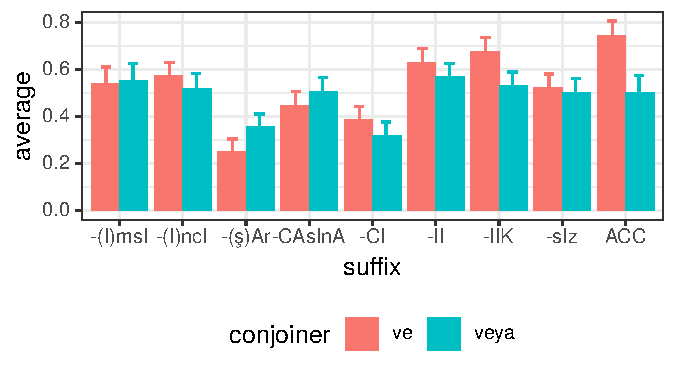
\includegraphics[]{experiments/acceptability/report/figure/suffixacceptability-1.pdf} 

}

\caption[First experiment, average acceptability for SA of suffixes by conjoiner]{First experiment, average acceptability for SA of suffixes by conjoiner}\label{fig:suffixacceptability}
\end{figure}


\end{knitrout}

For more inference in the acceptabilities, I fit a linear mixed model to responses using Conjoiner and Suffix as predictors with random effects for subject and item. I give the results of the model in Figure \ref{fig:derivationalmodel}. The points indicate median estimates and the thick line represents \%50 dredible intervals and the thin line represents the \%95 credible intervals. The log-odd estimates above zero indicate increased odds of suspendability relative to the other derivational suffixes or conjoiner.

\begin{knitrout}
\definecolor{shadecolor}{rgb}{0.969, 0.969, 0.969}\color{fgcolor}\begin{figure}[hbt!]

{\centering 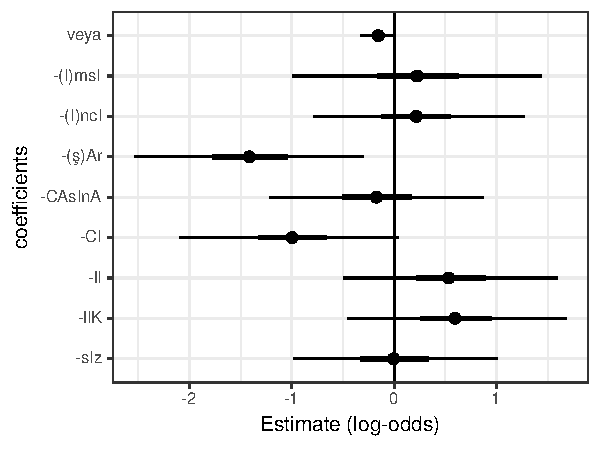
\includegraphics[]{experiments/acceptability/report/figure/derivationalmodel-1.pdf} 

}

\caption[First experiment, model results fit to grammaticality judgments with the predictors Suffix(8 derivational|1 inflectional) and Conjoiner(ve|veya)]{First experiment, model results fit to grammaticality judgments with the predictors Suffix(8 derivational|1 inflectional) and Conjoiner(ve|veya)}\label{fig:derivationalmodel}
\end{figure}


\end{knitrout}

\subsection{Analysis}


Figure \ref{fig:derivationalmodel} shows wide posterior probability distributions for the coefficients. One of the reasons for this is the low item count for each suffix. Another reason can be the varying degree of behaviour among the participants. The conjoiner choice of \textit{veya} "or" decreases the acceptability for SA in general. It also shows that suffixes do not behave uniformly in terms of acceptability. The suffixes \textit{-lI} and \textit{-lIK} seem to have the highest acceptabilities among all derivational suffixes, trailed by \textit{-(I)ncI} and \textit{-(I)msI}. There is no particular grouping of derivational suffixes in terms of acceptability. Positive estimates in this case don't indicate suspendability being grammatical or not, it is just a comparison made relative to a grand mean.

The two suffixes \textit{-(I)ncI} and \textit{-(ş)Ar} take numerals as their base and they both derive a nominal. They differ in average acceptability and the model results indicate a very small overlap in credible intervals. The suffix \textit{-CAsInA} takes participle forms as its base\footnote{it can take simple nouns too, but all the examples in the experiments are participle forms.} and  participle forms can end sentences with {\Tsg} interpretation in Turkish. This indicates that such bases are already assigned a lexical category. 

The varying degree of average acceptabilities among derivational suffixes and the similar results of the model show that SA of derivational suffixes in Turkish does not rely on a morphological phase analysis. If such an analysis were to hold true, the suffixes that take the same base should have behaved the same and the suffix taking participle base should have faired better. If a morphological phase analysis is not viable according to the experiment results, an approach that could capture the varying degree of acceptability is needed. The approach I take is the frequencies of the suffixes. For this purpose I extracted the frequencies of all four derivational suffixes (\textit{-lI,-lIK,-sIz}, and \textit{-CI} that TS Corpus \citep{sezer2013ts} had parsed). I give the relative proportion of the suffixes in Figure \ref{fig:suffixcorpus}. 

\begin{knitrout}
\definecolor{shadecolor}{rgb}{0.969, 0.969, 0.969}\color{fgcolor}\begin{figure}[hbt!]

{\centering 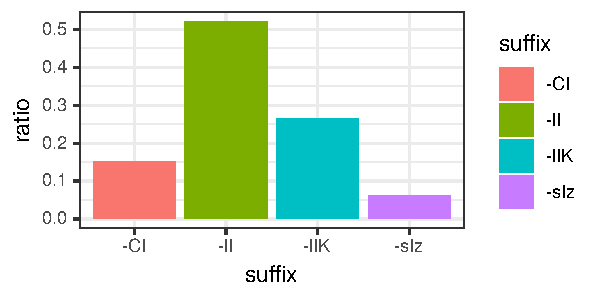
\includegraphics[]{experiments/acceptability/report/figure/suffixcorpus-1.pdf} 

}

\caption[Relative proportion of derivational suffixes in TS Corpus]{Relative proportion of derivational suffixes in TS Corpus}\label{fig:suffixcorpus}
\end{figure}


\end{knitrout}

The suffixes with the highest acceptabilities were \textit{-lI} and \textit{-lIK}. These two are the first two most frequent suffixes among the four presented in Figure \ref{fig:suffixcorpus}. Unfortunately not all derivational suffixes are readily extractable from the corpus data. The relative frequency of the suffixes in the corpus is not equally reflected by the experiment results and the experiment results indicate \textit{-CI} being less likely to be suspended compared to \textit{-sIz} even though it is relatively more frequent in the corpus.

The experiment results do not reflect the order of relative frequencies of these suffixes. The suffixes \textit{-lI} and \textit{-lIK} indeed have the highest acceptabilities in the experiment results, yet they aren't to the proportions of their relative frequencies. The suffix \textit{-CI} is relatively more frequent compared to \textit{-sIz} but fairs less acceptable in the experiment results. This means that raw frequency of a morpheme is not enough to explain the results. The two suffixes \textit{-(I)ncI} and \textit{-(I)msI} might hold an answer. These two suffixes receive similar acceptabilities with close estimates and overlapping credible intervals. 

I made a search in TS Corpus \citep{sezer2013ts} for examples of SA of the two suffixes \textit{-(I)ncI} and \textit{-(I)msI}. I provide two small CQP search keys \citep{hardie2012cqpweb}\footnote{CQP notation lets the user combine multiple features for a word in a corpus. These features include things like lexical category and morphological composition, together with regular expressions to specify certain character strings. A hit means a positive result matching the provided search key, and not all hits mean examples of suspended affixation.} in (\ref{tsinciquerry}) for SA of \textit{-(I)ncI}, with the numbers ranging from one to ten, and for \textit{-(I)msI} with noun and adjective bases.

\begin{exe}
\ex \label{tsinciquerry}
\begin{xlist}
\ex \label{inciquerry}\textit{-(I)ncI} TS corpus search key\\*
{[word="(bir{\textbar}iki{\textbar}üç{\textbar}dört{\textbar}beş{\textbar}altı{\textbar}yedi{\textbar}sekiz{\textbar}dokuz{\textbar}on)"][word="ve"]}
{[word="(.+nc(ı{\textbar}i{\textbar}u{\textbar}ü))"]}

\ex \textit{-(I)msI} TS corpus search key\\*
{[PosTag="Noun{\textbar}Adj"][word="ve"][PosTag="Adj" \& word="(.+ms(ı{\textbar}i{\textbar}u{\textbar}ü))"]}
\end{xlist}
\end{exe}

There are many examples for the SA of \textit{-(I)ncI} within $\sim$500 hits. The same can not be said for \textit{-(I)msI} which has the same acceptance rate as \textit{-(I)ncI} but the corpus search does not result in an SA of \textit{-(I)msI} within $\sim$500 hits. This discrepancy between similar acceptabilities but different corpus results can be explained by the relative frequency of these suffixes according to the context they are used in. The examples for SA of \textit{-(I)ncI} mostly comprise of texts written by clerks or reporters that refer to the passage or paragraph numbers of a law. In (\ref{corpusquerry}), I give some partial examples from the corpus search results for (\ref{inciquerry}). 

\begin{exe}
\ex SA of \textit{-(I)ncI} in corpus\\*
\label{corpusquerry}
\begin{xlist}

\ex \gll \ldots hüküm-ler bir ve iki-nci fıkra-lar-da yeniden düzenlendiğinden \ldots \\
\ldots provision-{\Pl} one {\And} two-{\Der} paragraph-{\Pl}-{\Loc} again change.because \ldots \\
\glt `\ldots because the provisions were adjusted again in the first and second paragraphs \ldots'

\ex \gll \ldots kanun-un dört ve beş-inci madde-ler-i değiş-tir-il-miş \ldots \\
\ldots law-{\Gen} four {\And} five-{\Der} article-{\Pl}-{\Poss}.{\Tsg} change-{\Caus}-{\Pass}-{\Prf}[{\Tsg}] \ldots \\
\glt`{\ldots} the forth and the fifth articles of the law were changed {\ldots}'

\end{xlist}
\end{exe}

There are examples in texts related to football, education, and others but texts related to law are more prominent. Unfortunately, text types are not tagged in TS Corpus. That's why it is hard to identify which text belongs to which context. I made a pseudo classification for the search results with the text categories of law, football, education, and others. I made the categorization depending on what the twenty words before and after the search hit contained. If those words contained an inflected or derived form of some words they are categorized according to the list of words they match. In (\ref{categorylist}), I provide what words defined a category of text. If twenty word periphery of the search hit contained an inflected or derived word outside the lists, it is categorized as `others'. This resulted in the classification of total 513 hits into 229 counts of law, 175 counts of others, 58 counts of education, and 51 counts of football in terms of what context the hit was in. This means that texts that are related to `law' are more numerous, thereby they are more likely to host examples for SA of \textit{-(I)ncI}.

\begin{exe}
\ex \label{categorylist}
\begin{xlist}
\ex Law: \textit{kanun, hüküm, fıkra, madde, paragraf, yönetmelik, nüsha}
\glt `law, provision, paragraph(archaic), article, paragraph, regulations, copy(archaic)'

\ex Football: \textit{gol, takım, lig, futbol, puan, oyun}
\glt `goal, team, football, point, game'

\ex Education: \textit{sınıf, ders, okul, eğitim, öğrenci}
\glt `class, course, school, education, student'

\end{xlist}
\end{exe}


\subsection{Conclusion}
The results of the experiment, comparisons of some derivational suffixes, and the related corpus searches provide two main observations about the suspendability of derivational suffixes. First, purely theoretical explanations can't predict varying acceptabilities. Second, suffixes with similar acceptabilities do not result in similar number of examples in the corpus. Taking these observations into consideration, I propose the following: The acceptability for SA of a derivational suffix is related to the relative frequency of the suffix given the context it is used in. Additionally the conjoiner \textit{veya} `or' decreases acceptability for all suffixes.

















\section{Experiment 2}

The aim of this experiment is to see what the cost of SA in a local environment is and if it is additive by the number of suffixes using a self-paced reading study. A local environment means that the target conjunct and the source conjunct for the suspended affix(es) are in the adjacent periphery of the conjoiner. Target conjunct is where the affix is interpreted but phonologically covert and the source conjunct is where it is overt. In the case of Turkish, the source conjunct is the rightmost conjunct as illustrated in (\ref{templateforsuspension}).

\begin{exe}
\ex \label{templateforsuspension}
CONJ1$_{target}$ (conjoiner) CONJ2$_{source}$ 
\end{exe}

SA in the nominal domain is ambiguous except than the SA of {\Case}. SA in the verbal domain, on the other hand, does not result in ambiguity, and the SA capable suffixes can be stacked. This enables me to test the effects, if any, of suspending different number of suffixes. In addition to changing the amount of suffixes, I investigate if the acceptability decreasing effect of the conjoiner \textit{veya} `or' in the first experiment will be reflected by increases in reading times.

There is one concern with using verbal domain for SA. The target conjunct can only be reduced to a verb plus a participle morpheme. These participle morphemes can have {\Tsg} agreement interpretations on their own. Should an effect arise in SA amount changes, it might be related to the mismatches between the first and second conjuncts instead of SA. There are additional conditions to meet this concern. These conditions are formed by changing an aspect or agreement of the first conjunct. This provides a contrast in terms of distinguishing an effect of suspension from feature mismatches. I lay out the experiment and analysis of the results in the following subsections.


\subsection{Participants}

The participants were 160 students from Boğaziçi University who are native speakers of Turkish. In exchange for their participation they received 1 point to their overall course score with the consent of the course's instructor.


\subsection{Materials}

The experiment comprised of three variables. The first variable was the Amount of SA with the levels: No SA, One SA, and Full SA.
In No SA, no suffix is suspended. In One SA, only one suffix is suspended. In Full SA, two suffixes are suspended. The second variable is the Conjoiner with the levels: \textit{ve} `and' and \textit{veya} `or'. The third variable is Contrast with the levels: Contrast and Parallel (No SA). In this last variable one of the suffixes in the first conjunct is altered to have a grammatical feature mismatch between the conjuncts. This contrast is only performed on the No SA conditions. This resulted in an experiment design with 4x2 conditions combining the amount of SA and conjoiner type, plus two conditions where there is a contrasting first conjunct for No SA condition. There were 24 distinct items together with 48 filler items. All experimental and filler items were grammatical. A latin square design by condition was applied, forming 8 lists of 24. This resulted in each participant seeing only 24 experimental items and 48 fillers. All the experimental items had a four-word pre and four-word post conjunction regions. (\ref{selfpacedtemplate}) shows a template for an experimental item. In (\ref{selfpacedexamples}), I give an example set of experimental items with all the conditions. All the experimental items and fillers had a comprehension question with half of them having "yes" and the other half having "no" as the correct answer. I carried out the experiment using ibexfarm \citep{drummond2013ibex}. For the full list of items and fillers (1-24 and 100-148) see Appendix \ref{selfpaceditems}.

\begin{exe}
\ex \label{selfpacedtemplate}
4WORDS CONJ1-$\alpha$-$\beta$ \textit{ve/veya} CONJ2-$\alpha$-$\beta$ 4WORDS

\ex \label{selfpacedexamples}
    \begin{xlist}
  \ex No SA:{\And}/{\Or}\\* 
  \gll \ldots yap-sa-ymış-ım ve/veya gönder-se-ymiş-im \ldots \\ 
  \ldots do-{\Cond}-{\Prf}-{\Fsg} {\And}/{\Or} send-{\Cond}-{\Prf}-{\Fsg} \ldots \\
  \glt ${}$

  \ex One SA:{\And}/{\Or}\\*
  \gll \ldots yap-sa-ymış ve/veya gönder-se-ymiş-im \ldots \\ 
  \ldots do-{\Cond}-{\Prf} {\And}/{\Or} send-{\Cond}-{\Prf}-{\Fsg} \ldots \\
  \glt ${}$
  
  \ex Full SA:{\And}/{\Or}\\*
  \gll \ldots yap-sa ve/veya gönder-se-ymiş-im \ldots \\ 
  \ldots do-{\Cond} {\And}/{\Or} send-{\Cond}-{\Prf}-{\Fsg} \ldots \\
  \glt ${}$
  
  \ex Contrast:{\And}/{\Or}\\*
  \gll \ldots yap-sa-ymış-ız ve/veya gönder-se-ymiş-im \ldots \\ 
  \ldots do-{\Cond}-{\Prf}-{\Fpl} {\And}/{\Or} send-{\Cond}-{\Prf}-{\Fsg} \ldots \\
    \end{xlist}
\end{exe}


\subsection{Procedure}

Participants were provided with a link to the experiment prompting them with a consent page. Upon giving consent participants went through 5 practice items and then they were prompted again for the beginning of the experiment. Each trial proceeded by the participants pushing the "space" key, for each key stroke a word at the center of the screen appeared and by each key stroke it was replaced with the following word in the sentence. After the sentence was read, the participants were presented with a statement that was either true or false according to the sentence they read. The statement was made about a dependency that was formed within the sentence. This could have been a modification of a noun or the verb, or the argument relations within the sentence. Participants professed their decision by pushing "Q" key for "yes" and "P" key for "no" on the keyboard. The experiment only recorded word reading times, responses, and response times. After the experiment was done, the participants were redirected to a separate page where they provided their student information to be relayed to the course's professor for the extra credit. This is kept separate of the experiment results, keeping participant information and experimental data anonymous.

\subsection{Results}

The results were recorded onto a csv file and imported to R \citep{team2013r} for data cleaning, aggregation, and analysis. Two items with a typo are excluded from the data (they do not count in initial data points). The data consisted of 38720 points before cleaning. 4 articipants whose accuracies were below 70\% are excluded from the data. After these exclusions, 15.48\% of the trials which had incorrect answers for the comprehension question is excluded from data analysis. The trials in which a word had a reading time that was outside 100-3000 milliseconds were considered outliers and those trials are also excluded. The whole cleaning resulted in the loss of 25.03\% of the data. In Figure \ref{fig:secondplot}, I give the average reading times per word with a representative sentence for the conditions of suspension amount.

\begin{knitrout}
\definecolor{shadecolor}{rgb}{0.969, 0.969, 0.969}\color{fgcolor}\begin{figure}[hbt!]

{\centering 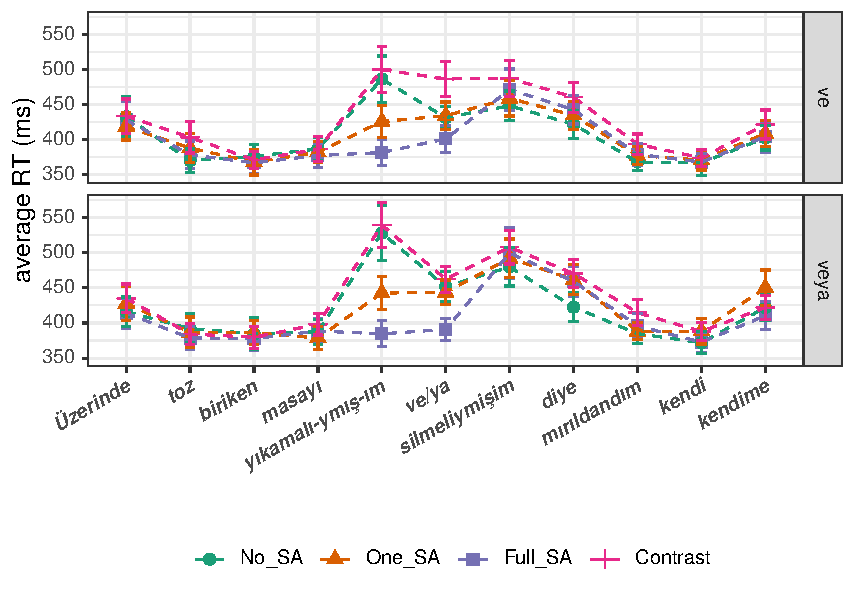
\includegraphics[]{experiments/selfpaced/report/figure/secondplot-1.pdf} 

}

\caption[Second experiment, average reading times of a sentence for all categories(No SA, One SA, Full SA, Contrast) and conjoiners(ve, veya)]{Second experiment, average reading times of a sentence for all categories(No SA, One SA, Full SA, Contrast) and conjoiners(ve, veya)}\label{fig:secondplot}
\end{figure}


\end{knitrout}

The critical region in all the sentences is the 7$^{th}$ word. In the case of Figure \ref{fig:secondplot} it is \textit{silmeliymişim} `(I) should have cleaned (something)'. The spillover region is the two words after the critical region. In this case the words \textit{diye} `saying that' and \textit{mırıldandım} ` (I) mumbled'. In Figure \ref{fig:thirdplot}, I give the average reading times of the critical and spillover region words by experimental conditions.

\begin{knitrout}
\definecolor{shadecolor}{rgb}{0.969, 0.969, 0.969}\color{fgcolor}\begin{figure}[hbt!]

{\centering 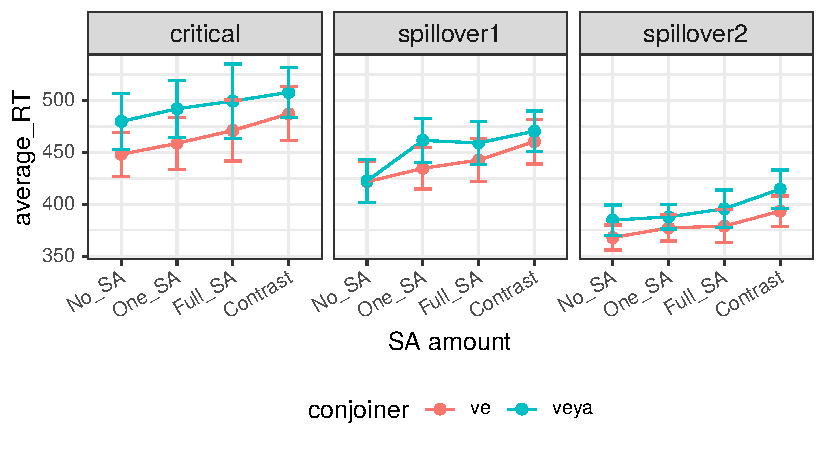
\includegraphics[]{experiments/selfpaced/report/figure/thirdplot-1.pdf} 

}

\caption[Second experiment, average reading times of critical and spillover regions for all categories(No SA, One SA, Full SA, Contrast) and conjoiners(ve, veya)]{Second experiment, average reading times of critical and spillover regions for all categories(No SA, One SA, Full SA, Contrast) and conjoiners(ve, veya)}\label{fig:thirdplot}
\end{figure}


\end{knitrout}

There is an increase in critical and spillover regions with the conjoiner \textit{veya} `or'. The amount of suspension does not display a similar trend in all the regions. In the critical region and the first spillover word, there is a slight increase by the number suspended suffixes. Contrasting sentences have higher reading times compared to suspension of one and two suffixes. This indicates that feature mismatches between the conjuncts lead to different processes other than SA.

For more inference on the effects of SA, I fit 3 linear mixed models for the reading times of the critical and spillover region words. I used SA amount and Conjoiner as predictors with random effects for subject and item. I used sliding differences contrasts for the SA amount, and sum contrast for the Conjoiner. Sliding differences mean that the comparisons are made between the levels of the differences. This follows from the expectation of varying effects depending on the SA amount, which is an incremental but not a categorical change. I give the models' results for SA amount in Figure \ref{fig:targetmodels}. The model results indicate an increase in spillover region for the suspension of one suffix, with no additive effects by suspending one more suffix. The conjoiner \textit{veya} `or' increased reading times consistently in all regions.

\begin{knitrout}
\definecolor{shadecolor}{rgb}{0.969, 0.969, 0.969}\color{fgcolor}\begin{figure}[hbt!]

{\centering 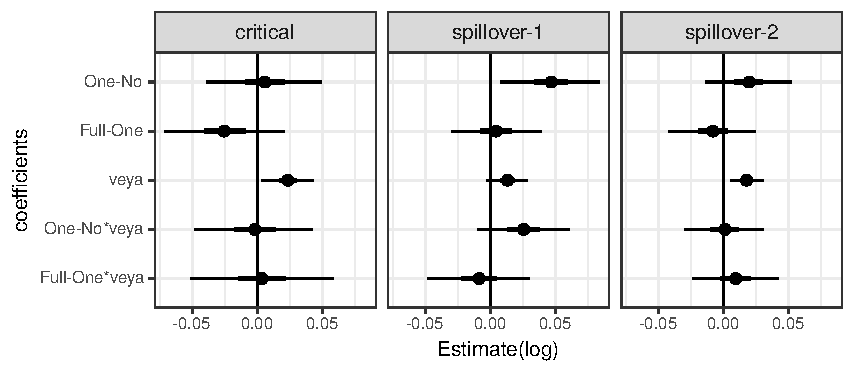
\includegraphics[]{experiments/selfpaced/report/figure/targetmodels-1.pdf} 

}

\caption[Second experiment, model results for the SA amount conditions fit to reading times with the predictors SA amount(No SA-One SA-Full SA) and Conjoiner(ve, veya)]{Second experiment, model results for the SA amount conditions fit to reading times with the predictors SA amount(No SA-One SA-Full SA) and Conjoiner(ve, veya)}\label{fig:targetmodels}
\end{figure}


\end{knitrout}

In addition to the effects of SA, I fit another 3 models for the reading times of the critical and spillover region words using feature match between conjuncts and conjoiner as predictors with random affects for subject and item. I used sliding difference for feature match, comparing Contrast to No SA, and sum contrast for the conjoiner. The results indicate an increase in reading times in Contrast conditions (Contrast, No SA) in all regions, with an increase in reading times by the conjoiner \textit{veya} `or' only in the critical region and the second spillover region word.

\begin{knitrout}
\definecolor{shadecolor}{rgb}{0.969, 0.969, 0.969}\color{fgcolor}\begin{figure}[hbt!]

{\centering 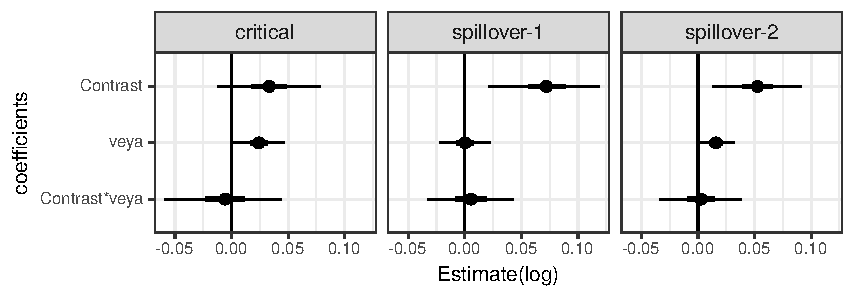
\includegraphics[]{experiments/selfpaced/report/figure/contrastmodels-1.pdf} 

}

\caption[Second experiment, model results for the feature mismatching conjuncts fit to reading times with the predictors Contrast(Contrast, No SA) and Conjoiner(ve, veya)]{Second experiment, model results for the feature mismatching conjuncts fit to reading times with the predictors Contrast(Contrast, No SA) and Conjoiner(ve, veya)}\label{fig:contrastmodels}
\end{figure}


\end{knitrout}

Figures \ref{fig:targetmodels} and \ref{fig:contrastmodels} indicate that suspending an affix and feature mismatches between conjuncts increase reading times. I fit 3 other models to compare only One SA and Contrast conditions in all the regions with random effects for subject and item. This time I used sum contrasts across the board. If the two levels behave the same, the comparison should result in indifference between One SA and Contrast. I give the models' results in Figure \ref{fig:saVcontrast}. The results indicate increased reading times in Contrast conditions compared to One SA. This differentiates the operation of SA and feature mismatches between the conjuncts.

\begin{knitrout}
\definecolor{shadecolor}{rgb}{0.969, 0.969, 0.969}\color{fgcolor}\begin{figure}[hbt!]

{\centering 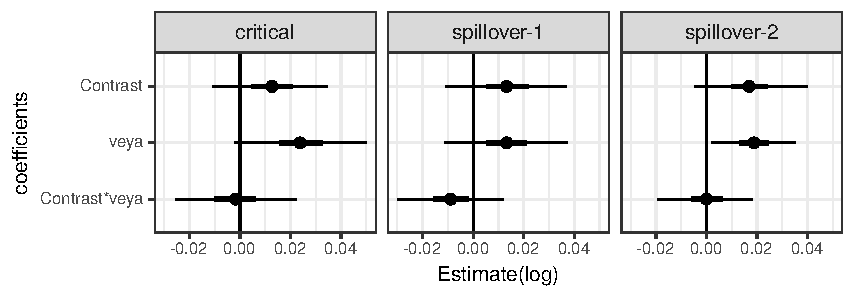
\includegraphics[]{experiments/selfpaced/report/figure/saVcontrast-1.pdf} 

}

\caption[Second experiment, model results for the comparison of suspending an affix (One SA) and feature mismatching conjuncts (Contrast) fit to reading times with the predictors of Category(Contrast-One SA) and Conjoiner(ve, veya)]{Second experiment, model results for the comparison of suspending an affix (One SA) and feature mismatching conjuncts (Contrast) fit to reading times with the predictors of Category(Contrast-One SA) and Conjoiner(ve, veya)}\label{fig:saVcontrast}
\end{figure}


\end{knitrout}

\subsection{Analysis}

In this experiment, the main aim was to identify the cost of SA. The results indicate that suspending a suffix is costly but it is not additive. The conjoiner \textit{veya} `or' increased reading times, this is a similar trend of decreasing acceptabilities in the first experiment. The feature mismatches between the conjuncts also lead to increased processing cost but they are greater than those of suspension. In the first experiment this effect is directly realted to SA, because the response was directly related to SA. In this experiment the main effect of the conjoiner in reading times can not be tied to SA. An increase in reading times can be caused by the semantic difference between the two conjoiners \textit{ve} `and' and \textit{veya} `or'. This means that the conjoiner effect in this experiment is not related to SA directly. If there was such a relation, the conjoiner \textit{veya} `or' and the suspension conditions should have had an interaction effect, presumably an increase in reading times for suspending suffixes in an environment formed by the conjoiner \textit{veya} `or'.











\section{Conclusion of Experiments 1 and 2}

The first experiment was conducted in the nominal domain and the analyses were based on responses. It aimed to compare suspendability of derivational suffixes to the suspension of inflectional {\Acc}. The results and the analyses indicate that suspendability of derivational suffixes is less related to structural explanations than it is to the frequency of those suffixes. This does not mean, however, that a structural explanation is not required. If the context relative frequency of a suffix is given as an explanation, a more gradient measurement is needed. Additionally using a conjoiner \textit{veya} `or' decreased acceptability of SA overall, this needs to be addressed theoretically. I reserve the discussion of the conjoiner to Chapter 5.


The second experiment was conducted in the verbal domain and the analyses were made based on the reading times. It aimed at observing the effects of performing SA. It compared suspending different number of suffixes with using two different conjoiners for the environment. It made another comparison using contrasting features in the first conjunct to distinguish an effect of SA from an effect of feature mismatch between the conjuncts. The results and the analyses indicate that performing SA is costly but not additive. The cost of performing SA is different than an effect of mismatching features between the conjuncts. 











\chapter{\MakeUppercase{Data}}
% to reset the gb4e example count for each chapter



\chapter{\MakeUppercase{Analysis}}
% to reset the gb4e example count for each chapter


In this chapter I first evaluate the results of the experiments and their implications. Later I present my arguments for SA related issues regarding some morphemes and their theoretical interpretations. 


\section{Suspended affixation and \textit{ile/=(y)lA}} \label{sec:ile}

In this section, I present the clitic \textit{ile/=(y)lA} in Turkish that serves several functions. My aim is to show how the conjoiner function of this clitic relates to SA. I argue that \textit{ile/=(y)lA} is morphologically the conjoiner head but its phonological size includes the place where {\Case} is encoded. According to \cite{goksel2004turkish} \textit{ile/=(y)lA} can be used as a case marker and a conjoiner as in (\ref{ilefunctions}). Being a clitic, \textit{ile/=lA} is outside the phonological word and thereby unstressable.

\begin{exe}
    \ex \label{ilefunctions} 
    \begin{xlist}
    \ex Instrumental \label{ileins}\\*
    \gll Şişe-yi çakmak ile aç-tı.\\ 
    bottle-{\Acc} lighter {\Ins} open-{\Pst}[{\Tsg}] \\
    \glt `S/he opened the bottle with a lighter.'
    
    \ex Comitative \label{ilecomit}\\*
    \gll Ahmet ev-e Mehmet ile (birlikte) gel-di. \\
    A[{\Nom}] house-{\Dat} M {\Com} (together) come-{\Pst}[{\Tsg}] \\
    \glt `Ahmet came home (together) with Mehmet'
    
    \ex Conjoiner \label{ileconj}\\*
    \gll kitap ile kalem çok pahalı. \\
    book {\And} pencil very expensive \\
    \glt `The book and the pencil is very expensive.'
    \end{xlist}
\end{exe}

The first function of \textit{ile/=(y)lA} in (\ref{ileins}) is like a semantic case \cite{woolford2006lexical} that seemingly does not have a case assigner. The second function of \textit{ile/=(y)lA} in (\ref{ilecomit}) is like a semantic case that can have an overt or covert case assigner, a postposition, \textit{birlikte} `together'. The third function of \textit{ile/=(y)lA} in (\ref{ileconj}) is a conjoiner. I am only interested in the conjoiner function of the clitic \textit{ile/=(y)lA} ({\And}, and ={\And} in glosses). I give an example of SA with \textit{ile/=(y)lA} in (\ref{ileandSA}).

\begin{exe}
    \ex \label{ileandSA}
    \begin{xlist}
    \ex \gll Ahmet kitap=la kalem-ler-i al-dı. \\ 
    A[{\Nom}] book={\And} pencil-{\Pl}-{\Acc} take-{\Pst}[{\Tsg}] \\
    \glt `Ahmet took the books and the pencils.'\\*
    `Ahmet took the book and the pencils.'
    \end{xlist}
\end{exe}


\subsection{SA in \textit{ile/=lA} constructions}

SA of {\Pl}, or {\Poss} in the environment of the clitic \textit{ile/=(y)lA} is ambiguous like it is in a conjunction formed with \textit{ve} `and'. The clitic \textit{ile/=(y)lA} allows for insertion of {\Pl} and {\Poss} suffixes between itself and the noun it is attached to. It does not allow the insertion of {\Case} but it allows SA of them, as shown in (\ref{ileprops}).

\begin{exe}
\ex \label{ileprops}
    \begin{xlist}
    \ex \gll *kitap-lar-ım-ı=ylA defter-ler-i al-dı-m. \\ 
    book-{\Pl}-{\Poss}.{\Fsg}-{\Acc}={\And} notebook-{\Pl}-{\Acc} take-{\Pst}-{\Fsg} \\

    \ex \gll kitap-lar-ım=lA defter-ler-i al-dı-m. \\ 
    book-{\Pl}-{\Poss}.{\Fsg}={\And} notebook-{\Pl}-{\Acc} take-{\Pst}-{\Fsg} \\
    \glt `I took my books and the notebooks.'
\end{xlist}
\end{exe}

As a general constraint, SA takes place for the rightmost terminal nodes. If the rightmost terminal node does not match the suspended affixes, SA does not take place. In (\ref{ileSA}) all the second conjuncts have the rightmost {\Pl-\Acc}. 

\begin{exe}
    \ex \label{ileSA}
    \begin{xlist}
        \ex \label{ilesa1}\gll Kalem=le kitap-lar-ı al. \\ 
        pencil={\Case} book-{\Pl}-{\Acc} take.{\Imp} \\
        \glt `Take the pencils and the books'
        
        \ex \label{ilesa2}\gll Kalem ve kitap-lar-ı al. \\ 
        pencil {\And} book-{\Pl}-{\Acc} take.{\Imp} \\
        \glt `Take the pencils and the books'
    \end{xlist}
\end{exe}

If the clitic \textit{ile/=lA} in (\ref{ilesa1}) were to be a case marker, it would mismatch with {\Acc}. This should have stopped SA of {\Pl}. This is not the case and both sentences in (\ref{ileSA}) are examples of SA. There is no SA environment in Turkish that violates the rightward-bound process of deletion, and positing \textit{ile/=(y)lA} as an exception is not needed if an explanation that captures both the SA capability and inability of {\Case} insertion can be given. The examples in (\ref{ileSA}) would violate the rightward-bound nature of SA since {\Poss} and {\Pl} suffixes before \textit{ile/=(y)lA} would be subject to suspension but not \textit{ile/=(y)lA} itself. I argue that, in its conjoiner function, \textit{ile/=(y)lA} itself is a conjoiner head and not a case mark assigned by a zero conjoiner head.


\subsection{What does \textit{ile/=lA} conjoin?}

The phrase that \textit{ile/=(y)lA} conjoins is not marked for {\Case}, yet it can be marked for number and possession. The first approach to conjoiner \textit{ile/=(y)lA} can use the insertable and non-insertable suffixes to determine the size of a conjunct for \textit{ile/=(y)lA}. In \S \ref{SAanalysisproposal} I proposed to place both number and agreement suffixes on the small `n' head. If {\Case} can not be inserted before \textit{ile/=(y)lA} but number and possession can be, then it might be conjoining nPs. In Figure \ref{fig:ile}, I give a representation for \textit{ile/=(y)lA} conjoining nPs.

\begin{figure}[hbt!]
    \centering
    \begin{forest}
    for tree={inner sep=0}
    [nP 
        [BP 
            [nP 
                [NP]
                [n]]
            [B\\\textit{ile/=(y)lA}]]
        [nP 
            [NP]
            [n]]]
    \end{forest}
    \caption{Representation of \textit{ile/=(y)lA} as a conjoiner of nPs}
    \label{fig:ile}
\end{figure}

This analysis argues for a small conjunction of two inflectional levels before a DP layer and after the lexical item. One issue with this analysis comes about when the conjuncts are modified with a modifier that requires a DP layer. In Turkish, there is a suffix \textit{-ki} that is attached to {\Loc} marked nouns and it either derives an adjectival modifier or a pronominal. I give the examples in (\ref{kiexample}) to show the difference of adjectival \textit{-ki} than a normal adjectival modifier.

\begin{exe}
\ex \label{kiexample}
    \begin{xlist}
    \ex \label{kiexample1}
    \gll Ahmet küçük kitap bul-a-ma-dı. \\
    A[{\Nom}] small book find-{\Abil}-{\Neg}-{\Pst}[{\Tsg}] \\ 
    \glt `Ahmet bought some small book'

    \ex \label{kiexample2}
    \gll *Ahmet araba-da-ki kitap bul-a-ma-dı. \\ 
    A[{\Nom}] car-{\Loc}-ki book find-{\Abil}-{\Neg}-{\Pst}[{\Tsg}] \\
    
    \ex \label{kiexample3}
    \gll Ahmet araba-da-ki kitab-ı bul-a-ma-dı. \\ 
    A[{\Nom}] car-{\Loc}-ki book-{\Acc} find-{\Abil}-{\Neg}-{\Pst}[{\Tsg}] \\
\glt `Ahmet took the book in the car.'
\end{xlist}
\end{exe}

The nouns that are modified with an adjective can be non-referential as in (\ref{kiexample1}), but nouns that are modified with \textit{ki} derived modifiers can not be non-referential (\ref{kiexample2}). This shows that \textit{ki} modifiers require a position where the noun is already referential, and according to \cite{ozturk2002turkish} the DP layer is the place where referentiality is encoded. If the clitic \textit{ile/=(y)lA} were to be analyzed as in Figure \ref{fig:ile}, \textit{ki} derived modifiers should have rendered (\ref{ilecomplex}) ungrammatical.

\begin{exe}
\ex \label{ilecomplex} 
\gll Ahmet masa-da-ki kitap=la vazo-da-ki çiçeğ-i getir-di. \\
A[{\Nom}] table-{\Loc}-ki book={\And} vase-{\Loc}-ki flower-{\Acc} bring-{\Pst}[{\Tsg}] \\
\glt`Ahmet brought the book on the table and the flower in the vase.'
\end{exe}

The structural interpretation of \textit{ile/=lA} now has a the following problem. The use of \textit{ile/=(y)lA} in (\ref{ileSA}) and (\ref{ilecomplex}) are uses of the clitic as a conjoiner morpheme and it does not allow {\Case} insertion. The \textit{ki} derived modifiers require a DP layer so positing a conjunction of nPs is not feasible. Additional support for DP level conjunction in \textit{ile/=(y)lA} comes from the nominalized sentences in Turkish. \textit{ile/=(y)lA} can conjoin two nominalized sentences as in (\ref{ilesentence}).

\begin{exe}
\ex \label{ilesentence} 
\gll Ben-im ev-e gel-me-m=le sen-in uyan-ma-n aynı an-da ol-ma-dı. \\ 
{\Fsg}-{\Gen} house-{\Dat} come-{\Nmlz}-{\Fsg}={\And} {\Ssg}-{\Gen} wake\_up-{\Nmlz}-{\Ssg} same moment-{\Loc} happen-{\Neg}-{\Pst}[{\Tsg}] \\
\glt`Me coming home and you waking up did not happen at the same time.'
\end{exe}

Following from all the observations, I argue that the inability to insert overt case markers before \textit{ile/=lA} does not stem from the lack of a DP layer or whether \textit{ile/=(y)lA} functions as {\Case}. It is rather based on the vocabulary insertion. I propose to consider \textit{ile/=(y)lA} as a conjoiner like \textit{ve} `and' that can conjoin DP level nouns, and its phonological size includes the DP head and the BP head. I provide Figure \ref{fig:ilefinal} for a final representation of my proposal ({\Acc} is just a placeholder, any other {\Case} is applicable). In this representation I show the phonological insertion for the morphemes. The DP head is still morphologically encoded with {\Case}, but its vocabulary insertion is overwritten by the clitic \textit{ile/=(y)lA} that serves as the BP head morphologically and syntactically.

\begin{figure}[hbt!]
    \centering
    \begin{forest} for tree= {sn edges, s sep=15mm}
    [DP 
        [BP 
            [DP
                [nP, s sep =10mm 
                    [NP]
                    [n\\{\Pl-\Poss}]]
                [D, name=D]]
            [B, name=B]]
        [DP]]
    \node[right=0em of D](case){[\Acc]};
    \node[fit= (D)(case), draw, ellipse, dashed, scale=0.8](phon){};
    \node[below=0em of phon](item){\textit{-(y)I}};
    \node[fit=(D)(item)(phon)(B), draw, thick, ellipse, dashed, scale=0.8, rotate=145](clitic){};
    \node[below right=6em of clitic](item2){\textit{ile/=(y)lA}};
    \end{forest}
    \caption{Conjoiner \textit{ile/=(y)lA} phonologically occupying conjoiner head and {\Case}}
    \label{fig:ilefinal}
\end{figure}

This analysis is against an approach that uses subset principle where a vocabulary item is inserted for a place that it contains the morphemes for. Figure \ref{fig:ilefinal} places the vocabulary item for the clitic \textit{ile/=lA} on `D' and `B' with granting it the morphological realization of only `B'. This is solved by a procedure of Impoverishment \citep{bonet1991morphology}, where a specific vocabulary item does not contain all the morphemes it is inserted for. This means that \textit{ile/=lA} always triggers an operation of impoverishment at vocabulary insertion, it morphologically represents `B' but occupies the phonological space for both `D' and `B'. A position class morphology \citep{inkelas1993nimboran,stump1993position} in this case might not be helpful, since the conjoiner head is not an inflection on the noun but a clitic that needs a phonological host.

\section{Analysis of the suffix \textit{-(y)Ip}} 

In this section, I discuss the status of the suffix \textit{-(y)Ip} ({\Pc} in glosses). I give the structural interpretations that it should be evaluated under and the properties of the environment it forms. I argue for it to be evaluated as an environment of conjunction where SA beyond a morphological word is carried out.

\subsection{What is \textit{-(y)Ip}}

The suffix \textit{-(y)Ip} is used with verbs and only allows bare verbs, Voice, Mod$_{Abil}$, Negation, and the  suffix \textit{-(y)Iver} (I take this as Asp$_{Con}$ \citep{cinque1999adverbs} and mark as {\Con} in glosses) before it.  In (\ref{ipintro}), I give a set of examples for \textit{-(y)Ip}.

\begin{exe}
    \ex \label{ipintro}
    \begin{xlist}
    \ex Bare verb\\*
    \gll Ahmet koş-up düş-tü. \\ 
    A[{\Nom}] run-{\Pc} fall-{\Pst}[{\Tsg}] \\
    \glt `Ahmet ran and fell.'
    
    \ex verb-{\Caus}\\*
    \gll Ahmet şişe-yi dol-dur-up temizle-di. \\
    A[{\Nom}] bottle-{\Acc} fill-{\Caus}-{\Pc} clean-{\Pst}[{\Tsg}]\\
    \glt `Ahmet filled the bottle and cleaned it.'
    
    \ex verb-{\Abil}\\*
    \gll Ahmet mantıklı düşün-ebil-ip sorun-u çöz-dü. \\ 
    A[{\Nom}] sensible think-{\Abil}-{\Pc} problem-{\Acc} solve-{\Pst}[{\Tsg}] \\
    \glt `Ahmet was able to think sensibly and solved the problem.'
    
    \ex verb-{\Neg}\\*
    \gll Ahmet ev-e gel-me-yip bekle-di. \\
    A[{\Nom}] house-{\Dat} come-{\Neg}-{\Pc} wait-{\Pst}[{\Tsg}] \\
    \glt`Ahmet did not come home and waited.'
    
    \ex verb-{\Con}\\*
    \gll Ahmet bulaşıklar-ı yıka-yıver-ip otur-du. \\
    A[{\Nom}] dishes-{\Acc} wash-{\Con}-{\Pc} sit-{\Pst}[{\Tsg}]\\
    \glt `Ahmet managed to wash the dishes and sat down.'
    
    
    \ex verb-{\Abil}-{\Neg}-{\Con}\\*
    \gll Ahmet tutun-a-ma-yıver-ip düş-tü. \\ 
    A[{\Nom}] hold-{\Abil}-{\Neg}-{\Con}-{\Pc} fall-{\Pst}[{\Tsg}]\\
    \glt`Ahmet could not manage to hold on and fell.'
    \end{xlist}
\end{exe}

There are several arguments for its structural interpretation but they mainly boil down to converb adverbial \citep{demir2014adverbial, underhill1976turkish, goksel2004turkish}, and converb conjoiner \citep{fokkens2009inflectional, johanson1995turkic, kornfilt1997turkish} analyses. In this subsection, I show whether \textit{-(y)Ip} is a conjoiner or an adverbial. The sentences in (\ref{ipintro}) show that \textit{-(y)Ip} can conjoin two predicates that do not match in their Voice, Modality, and Polarity features. One contrasting behaviour of \textit{-(y)Ip} compared to other adverbial markers \textit{-(y)IncA} and \textit{-mAdAn} is given in (\ref{ipcontrast}). Under the same argument settings, \textit{-(y)Ip} is unacceptable\footnote{Contrasting subjects are grammatical with \textit{-(y)Ip} but they require changes in information structure, otherwise they are unacceptable. Exact grammatical considerations for \textit{-(y)Ip} constructions will be addressed in \S\ref{moreonyip}.} unlike \textit{-(y)IncA} and \textit{-mAdAn} ({\Pc}, {\When}, and {\Wo} in glosses respectively).

\begin{exe}
    \ex \label{ipcontrast}
    \begin{xlist}
        \ex \gll Ahmet koş-unca Mehmet düş-tü. \\ 
        A[{\Nom}] run-{\When} M[{\Nom}] fall-{\Pst}[{\Tsg}] \\
        \glt `When Ahmet ran, Mehmet fell.'
        
        \ex \gll Ahmet koş-madan Mehmet düş-tü. \\
        A[{\Nom}] run-{\Wo} M[{\Nom}] fall-{\Pst}[{\Tsg}] \\
        \glt `Mehmet fell before Ahmet ran.'
        
        \ex \gll ??Ahmet koş-up Mehmet düş-tü. \\ 
        A[{\Nom}] run-{\Pc} M[{\Nom}] fall-{\Pst}[{\Tsg}] \\
        \glt Intended `Ahmet ran and Mehmet fell.'
    \end{xlist}
\end{exe}

An objection to this observation can come from the adverbial suffix \textit{-(y)ArAK} `$\sim$ by Ving' ({\By} in glosses). It results in the same ungrammaticality as in (\ref{ipcontester}).

\begin{exe}
    \ex \label{ipcontester}
    \begin{xlist}
    \ex \gll Ahmet koş-arak düş-tü. \\
    A[{\Nom}] run-{\By} fall-{\Pst}[{\Tsg}] \\
    \glt `Ahmet fell running'
    
    \ex \gll *Ahmet koş-arak Mehmet düş-tü. \\ 
    A[{\Nom}] run-{\By} M[{\Nom}] fall-{\Pst}[{\Tsg}] \\
    \end{xlist}
\end{exe}

\textit{-(y)Ip} deviates from \textit{-(y)ArAK} in verb-manner relation. The verb marked with \textit{-(y)ArAK} requires semantic compatibility with the main verb. If the derived reading with \textit{-(y)ArAK} is not semantically compatible as a manner for the main verb, the expression receives an odd meaning. Verbs that are marked with \textit{-(y)Ip} do not require such a compatibility of manner. Manner relations are usually carried out by adverbs and adverbial clauses. In (\ref{ipandarak}), the suffix \textit{-(y)ArAK} is bound by verb-manner interpretations just like any other adverb whereas \textit{-(y)Ip} is not.

\begin{exe}
    \ex \label{ipandarak}
    \begin{xlist}
        \ex \label{ipandarak1} 
        \gll Ahmet koş-up uyu-du. \\
        A[{\Nom}] run-{\Pc} sleep-{\Pst}[{\Tsg}] \\
        \glt `Ahmet ran and slept.'
        
        \ex \label{ipandarak2} 
        \gll \%Ahmet koş-arak uyu-du. \\ 
        A[{\Nom}] run-{\By} sleep-{\Pst}[{\Tsg}] \\
        \glt `\%Ahmet slept running.'
    \end{xlist}
\end{exe}


An additional contrast of \textit{-(y)Ip} comes about in word order configurations. \textit{-(y)Ip} does not allow a word ordering under same argument settings as an adverbial suffix like \textit{-(y)ArAK} would allow. (\ref{ipandwordorder}) shows some word orderings for \textit{-(y)Ip} and \textit{-(y)ArAK}\footnote{Remember that word order changes are not free of interpretation in Turkish, they result in different information settings. See  \citet{ozturk2002turkish} for word order and change effects in Turkish.}. In these word orderings, the verb marked with \textit{-(y)Ip} and the main verb need to stay as a unit for a grammatical sentence.

\begin{exe}
\ex \label{ipandwordorder}
\begin{xlist}
    \ex \begin{xlisti}
        \ex \gll Ahmet koş-up gel-di. \\ 
        A[{\Nom}] run-{\Pc} come-{\Pst}[{\Tsg}] \\
        
        \ex \gll *koş-up Ahmet gel-di. \\ 
        run-{\Pc} A[{\Nom}] come-{\Pst}[{\Tsg}] \\
        
        \ex \gll koş-up gel-di Ahmet. \\ 
        run-{\Pc} come-{\Pst}[{\Tsg}] A[{\Nom}] \\
        \glt `Ahmet ran and came.'
    \end{xlisti}
    
    \ex \begin{xlisti}
        \ex \gll Ahmet koş-arak gel-di. \\ 
        A[{\Nom}] run-{\By} come-{\Pst}[{\Tsg}] \\
        
        \ex \gll koş-arak Ahmet gel-di. \\ 
        run-{\By} A[{\Nom}] come-{\Pst}[{\Tsg}] \\
        
        \ex \gll koş-arak gel-di Ahmet. \\ 
        run-{\By} come-{\Pst}[{\Tsg}] A[{\Nom}] \\
        \glt `Ahmet came running.'
        \end{xlisti}
    \end{xlist}
\end{exe}

This difference in grammaticality does not mean that \textit{-(y)Ip} has to be adjacent to the main verb, but it means that any word ordering needs to take the verb marked with \textit{-(y)Ip} and the main verb as equivalent units. If the verb marked with \textit{-(y)Ip} were to be a unit of modification for the main verb, all word order changes should have resulted in reading differences rather than ungrammaticalities. I argue that the observations made here distinguishes \textit{-(y)Ip} from an adverbial forming suffix. In the following subsection, I lay out how \textit{-(y)Ip} is taken to be a conjoiner.


\subsection{What does \textit{-(y)Ip} conjoin}

In the literature where \textit{-(y)Ip} is evaluated as a conjoiner \citep{fokkens2009inflectional,johanson1995turkic,kornfilt1997turkish}, it is given the status of conjoining VPs. On first sight, the lack of any tense and agreement marker leads to evaluating \textit{-(y)Ip} as a conjoiner of VPs. Figure \ref{fig:ipconjoinerearly} illustrates this analysis.

\begin{figure}[hbt!]
    \centering
    \begin{forest}
    [VP 
        [BP 
            [VP]
            [B\\\textit{-(y)Ip}]]
        [VP]]    
    \end{forest}
    \caption{Early conjoiner analysis of \textit{-(y)Ip}}
    \label{fig:ipconjoinerearly}
\end{figure}

Conjoining only VPs might be warranted given the lack of overt inflections for the \textit{-(y)Ip} marked verb, but this analysis has couple of problems. First of which is the ability of \textit{-(y)Ip} marked verb to have inflectional suffixes of Negation, and Modality. These should immediately elevate the representation of VP to a higher structure. Not all inflectional markers are represented by overt heads, but the existence of them can be addressed cross-linguistically. The observations of \citet{cinque1999adverbs,cinque2001note} show that multiple inflectional levels for Tense, Aspect and Modality exist. These inflectional levels can have functional projections that take specific types of adverbs. These adverbs reside in the specifier position of the functional projections. For example, the two time adverbials \textit{bugün} `today' and \textit{yarın} `tomorrow' can occupy the specifier position of Tense$_{\Fut}$. If they are both used in one sentence, they form a complex adverbial that means `soon' as illustrated in (\ref{buyarin}).  

\begin{exe}
\ex \label{buyarin} 
\gll Ahmet bugün yarın kitab-ı al-ıp gel-ecek. \\ 
A[{\Nom}] today tomorrow book-{\Acc} take-{\Pc} come-{\Fut}[{\Tsg}] \\
\glt Ahmet will buy the book and come here soon.'
\end{exe}

This is easily predicted by an analysis of VP conjunction for \textit{-(y)Ip} and functional projection for Tense$_{\Fut}$ since a VP can later be marked with a single projection of tense and both adverbs occupy the same position and form a compound. The \textit{-(y)Ip} clause can have an adverb to itself that is different from the main verb. In (\ref{ipconjunctionstime}), I provide an example where \textit{-(y)Ip} marked verb and the main verb differ in their time adverbial. In (\ref{ipconjunctionstime}), performing a conjunction of VPs require only one inflectional projection of Tense$_{\Fut}$ but \textit{-(y)Ip} clause can have its own time adverbial different than the matrix clause.

\begin{exe}
\ex \label{ipconjunctionstime}
\gll Ahmet bugün kitab-ı al-ıp yarın defter-i kapla-yacak. \\
A[{\Nom}] today book-{\Acc} buy-{\Pc} tomorrow notebook-{\Acc} wrap-{\Fut}[{\Tsg}] \\
\glt `Ahmet will buy the book today and will wrap the notebook tomorrow.'
\end{exe}

Another functional projection that can be used to illustrate higher level of conjunction for \textit{-(y)Ip} comes from speech act adverbials. The two speech act adverbials \textit{dürüstçe} `frankly' and \textit{sinsice} `deviously' result in a semantically odd reading if they are used in one sentence. (\ref{dursin}) shows the resulting odd reading.

\begin{exe}
\ex \label{dursin} 
\gll \%Ahmet dürüstçe ve sinsice konuş-up davran-dı. \\ 
A[{\Nom}] frankly {\And} deviously talk-{\Pc} behave-{\Pst}[{\Tsg}] \\
\glt Intended: `Ahmet talked and behaved frankly and deviously.'
\end{exe}

Placing one of the adverbs under the \textit{-(y)Ip} marked verb and the other under the main verb does away with the odd reading in (\ref{dursin}). If the two speech adverbials were to occupy the same inflectional level, the example in (\ref{ipconjunctionsspeech}) should have been semantically odd.

\begin{exe}
\ex \label{ipconjunctionsspeech}
\gll Ahmet dürüstçe konuş-up sinsice davran-ıyor. \\
A[{\Nom}] frankly talk-{\Pc} deviously act-{\Prog}[{\Tsg}] \\
\glt `Ahmet is talking honestly but acting deviously.'
\end{exe}

All the observations here show that \textit{-(y)Ip} does not conjoin VPs but higher projections. According to \citet{cinque1999adverbs}, speech act adverbials are used with the functional projection Mood$_{speech\,act}$ that is higher than Tense and Aspect projections. I argue that \textit{-(y)Ip} is a conjoiner for full sentences. In the following subsection, I give my analysis for \textit{-(y)Ip} conjunctions.


\subsection{Analysis of \textit{-(y)Ip}}

Analyzing \textit{-(y)Ip} as a conjunction that conjoins full sentences requires the explanation for missing and non-insertable suffixes. These suffixes range from aspect markers to person agreement markers. I propose that \textit{-(y)Ip} is a result of vocabulary insertion after SA. The specific reason for why \textit{-(y)Ip} is chosen instead of a free form conjoiner like \textit{ve} `ve' is a morphological one. In a conjunction of two sentences, suspension of suffixes on the verb is performed and a non-morphological word is left. This results in the violation of the morphological word constraint. The verb after deletion of exponents can not stand on its own. That is why a bound form conjoiner like \textit{-(y)Ip} is inserted for the conjoiner head instead of a free form conjoiner \textit{ve} `ve'. This way I combine both conjoiner function of \textit{-(y)Ip} and the explanation for missing suffixes. I provide my analysis in Figure \ref{fig:ipanalysis}. In Turkish, there aren't overt suffixes for `C' that can be suspended in \textit{-(y)Ip} constructions, that is why they are not interpreted under SA. 

\begin{figure}[hbt!]
    \centering
\begin{forest} for tree= sn edges
    [CP 
        [BP 
            [CP 
                [TP 
                    [\ldots 
                        [\ldots]
                        [X\\\cancel{-$\alpha$}, name=innerx]]
                    [T\\\cancel{-$\beta$}, name=innert]]
                [C]]
            [B\\ \textit{-(y)Ip}]]
        [CP 
            [TP 
                [\ldots 
                    [\ldots]
                    [X\\-$\alpha$, name=outerx]]
                [T\\-$\beta$, name=outert]]
            [C]]]
\node[fit= (innerx)(innert), draw, ellipse, dashed, rotate=155, scale=.75](inner){};
\node[fit= (outerx)(outert), draw, ellipse, dashed, rotate=155, scale=.75](outer){};
\node[below right= 4em of inner](innerlabel){SA};
\node[below right= 4em of outer](outerlabel){Overt suffixes};
\draw[->, thick, dashed] (outerlabel) to[out=south, in=east] node[midway, fill=white]{\textsc{recover}}(innerlabel);
\end{forest}
    \caption{Structural analysis proposal for \textit{-(y)Ip}}
    \label{fig:ipanalysis}
\end{figure}


In (\ref{ipmultiple}), I provide multiple \textit{-(y)Ip} constructions that are the results of being left with non-morphological words after SA.

\begin{exe}
\ex \label{ipmultiple}
\gll Ahmet ev-e gel-ip soyun-up uyu-muş-tur. \\
A[{\Nom}] house-{\Dat} come-{\Pc} undress-{\Pc} sleep-{\Prf}-PROB[{\Tsg}] \\
\glt `Ahmet has probably come home, undressed, and slept.'
\end{exe}

In (\ref{deriveipmultiple}), I give the order of derivation that leads to SA beyond the morphological word and the multiple instances of \textit{-(y)Ip}.

\begin{exe}
\ex \label{deriveipmultiple}
\begin{xlisti}
\ex Conjunction of n many sentences, with matching rightmost suffixes $\beta$
\ex Delete the matching nodes\\
    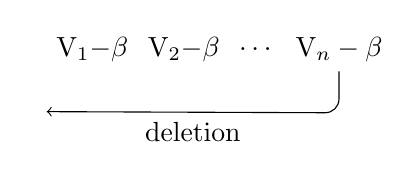
\begin{tikzpicture}
    \node[](leftr){};
    \node[right=0em of leftr](conj1){V$_1$\cancel{$-\beta$}};
    \node[right=0em of conj1](conj2){V$_2$\cancel{$-\beta$}};
    \node[right=0em of conj2](dots){\ldots};
    \node[right=0em of dots](conjn){V$_n-\beta$};
    \node[below=1.55em of leftr](leftcorner){};
    \draw[rounded corners=.5em, ->] (conjn.south) -- +(south:1.5em) -- node[below]{deletion}(leftcorner.east);
    \end{tikzpicture}
\ex The remnants are not morphological words, insert bound form conjoiner \textit{-(y)Ip}\\
    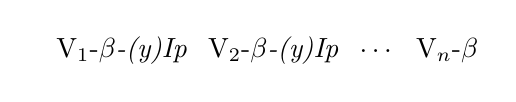
\begin{tikzpicture}
    \node[](leftrz){};
    \node[right=0em of leftrz](conj1){V$_1$\cancel{-$\beta$}\textit{-(y)Ip}};
    \node[right=0em of conj1](conj2){V$_2$\cancel{-$\beta$}\textit{-(y)Ip}};
    \node[right=0em of conj2](dots){\ldots};
    \node[right=0em of dots](conjn){V$_n$-$\beta$};
    \end{tikzpicture}
\end{xlisti}
\end{exe}


One possible problem for a conjoiner \textit{-(y)Ip} is its ability to co-exist with another conjoiner \textit{hem \ldots hem de \ldots} `both \ldots and \ldots' that seemingly carries out the function of the conjoiner \textit{ve} `and'. I do not take \textit{hem \ldots hem de \ldots} `both \ldots and \ldots' as a conjoiner but as focus particles that operate on the conjuncts. The counterpart \textit{ya \ldots ya da \ldots} `either \ldots or \ldots' that serves as the focus particle for the exclusive \textit{veya} `or' is ungrammatical. I give the example in (\ref{problemip}) to serve the point.

\begin{exe}
\ex \label{problemip} 
\begin{xlist}
\ex \gll hem tez yaz-ıp hem de çalış-mak ist-iyor-sun. \\ 
{\Foc} thesis write-{\Pc} {\Foc} {\Ptcp} work-{\Nmlz} want-{\Prog}-{\Ssg} \\
\glt `(You) want to both write your thesis and work.'

\ex \gll *ya tez yaz-ıp ya da çalış-mak ist-iyor-sun. \\ 
{\Foc} thesis write-{\Pc} {\Foc} {\Ptcp} work-{\Nmlz} want-{\Prog}-{\Ssg} \\

\ex \gll ya tez yaz-mak ya da çalış-mak ist-iyor-sun. \\  
{\Foc} thesis write-{\Nmlz} {\Foc} {\Ptcp} work-{\Nmlz} want-{\Prog}-{\Ssg} \\
\glt `You either want to write your thesis or you want to work.'
\end{xlist}
\end{exe}


In addition to its ability of co-existing with other conjoiner markers, \textit{-(y)Ip} can co-occur with the free form conjoiner \textit{ve} `and' as in (\ref{yipve}). These observations of \textit{-(y)Ip} co-existing with other conjoiners do not render a conjoiner analysis obsolete. There are many cases where conjoiners are used for the purposes of changing information structure in a sentence. What is important is that in both (\ref{problemip}) and (\ref{yipve}), \textit{-(y)Ip} is only grammatical in an environment where the interpretation of the sentence is equivalent to a conjunction formed by \textit{ve} `and'.

\begin{exe}
    \ex \label{yipve}
    \gll Ev-e gid-ip ve de anahtar-ı al-ma-mak tam bir aptallık. \\ 
    house-{\Dat} go-{\Pc} {\And} {\Foc} key-{\Acc} take-{\Neg}-{\Nmlz} complete a stupidity \\
    \glt `Going all the way home and not taking the key is a complete stupidity.'
\end{exe}


All the examples in the last two subsections distinguished \textit{-(y)Ip} from adverbial markers and presented it as a conjoiner of sentences. With these observations at hand, I propose that \textit{-(y)Ip} is a conjoiner that elevates the verb to a morphological word status. It does not occupy the morphological slots for the suspended suffixes, it surfaces after the suspension of affixes to satisfy the morphological word constraint. In the following subsection, I discuss why SA seems to be obligatory in \textit{-(y)Ip} constructions and why the environment of \textit{-(y)Ip} is important for the discussion of SA.


\subsection{Suspended affixation and \textit{-(y)Ip}} \label{sec:SAandyip}

A morphological word is defined if the last morpheme can terminate a sentence independent of agreement markers \citep{kabak2007turkish}. After SA in verbs, the conjoiner \textit{`ve'} is selected if what is left is a morphological word and the conjoiner \textit{-(y)Ip} is selected if what is left after SA is not a morphological word. 

This means that insertion for the conjoiner is dependent on the morphological status of what is left after SA. I give a set of examples in (\ref{ipandsa}) that show that SA is grammatical in verbs with non-morphological word status if the conjoiner is \textit{-(y)Ip} and SA is grammatical in verbs with morphological word status if the conjoiner is \textit{ve} `and'.

\begin{exe}
\ex \label{ipandsa}
\begin{xlist}
\ex \begin{xlisti}
\ex Non-morphological word, \textit{ve} `and'\\*
\gll *kitab-ı oku ve anla-malı-ydı-m. \\ 
book-{\Acc} read {\And} understand-{\Nec}-{\Pst}-{\Fsg} \\
\glt ${}$

\ex Non-morphological word, \textit{-(y)Ip}\\*
\gll kitab-ı oku-yup anla-malı-ydı-m. \\ 
book-{\Acc} read-{\Pc} understand-{\Nec}-{\Pst}-{\Fsg} \\
\glt `I should have read and understood the book.'
\end{xlisti}

\ex \begin{xlisti}
\ex Morphological word, \textit{ve} `and'\\* 
\gll kitab-ı oku-malı ve anla-malı-ydı-m. \\ 
book-{\Acc} read-{\Nec} {\And} understand-{\Nec}-{\Pst}-{\Fsg} \\
\glt `I should have read and understood the book.'

\ex Morphological word, \textit{-(y)Ip}\\*
\gll *kitab-ı oku-malı-yıp anla-malı-ydı-m. \\ 
book-{\Acc} read-{\Nec}-{\Pc} understand-{\Nec}-{\Pst}-{\Fsg} \\
\glt ${}$
\end{xlisti}
\end{xlist}
\end{exe}

The sentences in (\ref{ipandsa}) show that the vocabulary item for the conjoiner head is selected after SA is performed. This also explains why the suffixes \textit{-mA} and \textit{-(y)Abil} can reside under the conjoiner \textit{-(y)Ip} because they do not form morphological words. I give a set of examples in (\ref{negabilip}).

\begin{exe}
\ex \label{negabilip}
\begin{xlist}
\ex {\Abil} \begin{xlisti}
\ex \gll *kitab-ı oku-yabil ve anla-yabil-miş-im. \\ 
book-{\Acc} read-{\Abil} {\And} understand-{\Abil}-{\Prf}-{\Fsg} \\
\glt ${}$

\ex \gll kitab-ı oku-yabil-ip anla-yabil-miş-im. \\ 
book-{\Acc} read-{\Abil}-{\Pc} understand-{\Abil}-{\Prf}-{\Fsg} \\
\glt `It seems like I was able to read and understand the book.'
\end{xlisti}

\ex {\Abil-\Prf} \begin{xlisti}
\ex \gll kitab-ı oku-yabil-miş ve anla-yabil-miş-im. \\ 
book-{\Acc} read-{\Abil}-{\Prf} {\And} understand-{\Abil}-{\Prf}-{\Fsg} \\
\glt `It seems like I was able to read and understand the book.'

\ex \gll *kitab-ı oku-yabil-miş-ip anla-yabil-miş-im. \\ 
book-{\Acc} read-{\Abil}-{\Prf}-{\Pc} understand-{\Abil}-{\Prf}-{\Fsg} \\
\glt ${}$
\end{xlisti}

\ex {\Neg} \begin{xlisti}
\ex \gll *kitab-ı oku-ma ve anla-ma-mış-ım. \\ 
book-{\Acc} read-{\Neg} {\And} understand-{\Neg}-{\Prf}-{\Fsg} \\
\glt ${}$

\ex \gll kitab-ı oku-ma-yıp anla-ma-mış-ım. \\ 
book-{\Acc} read-{\Neg}-{\Pc} understand-{\Neg}-{\Prf}-{\Fsg} \\
\glt `It seems like I haven't read the book and understood it.'
\end{xlisti}

\ex {\Neg-\Prf}\begin{xlisti}
\ex \gll kitab-ı oku-ma-mış ve anla-ma-mış-ım. \\ 
book-{\Acc} read-{\Neg}-{\Prf} {\And} understand-{\Neg}-{\Prf}-{\Fsg} \\
\glt `It seems like I haven't read the book and understood it.'
\ex \gll *kitab-ı oku-ma-mış-ıp anla-ma-mış-ım. \\ 
book-{\Acc} read-{\Neg}-{\Prf}-{\Pc} understand-{\Neg}-{\Prf}-{\Fsg} \\

\end{xlisti}
\end{xlist}
\end{exe}

One prediction of my analysis for SA where \textit{-(y)Ip} is present is that ambiguous cases of SA should be possible if what is left after SA is still not a morphological word. I provide such an ambiguity in (\ref{ipambiguity}). In this example, SA of {\Neg} is optional since its existence or lack of it in the first conjunct does not change the morphological word status of the conjunct.

\begin{exe}
\ex \label{ipambiguity} 
\gll Ahmet ev-e gel-ip kitab-ı oku-ma-dı. \\ 
A[{\Nom}] house-{\Dat} come-{\Pc} book-{\Acc} read-{\Neg}-{\Pst}[{\Tsg}] \\
\glt `Ahmet did not come home and did not read the book.'\\*
`Ahmet came home but did not read the book.'
\end{exe}

If SA is performed for the suffixes {\Neg}-{\Pst}[{\Tsg}] which is all the way to the bare verb itself, you get the first reading of (\ref{ipambiguity}). If SA is performed for {\Pst}[{\Tsg}], you get the second reading of (\ref{ipambiguity}). In both readings, what is left after SA is not a morphological word since neither can {\Neg} nor a bare verb can terminate a sentence independent of agreement markers. This results in the selection of \textit{-(y)Ip} as a conjoiner. Figure \ref{fig:ambiguousip} represents the two readings of (\ref{ipambiguity}).

\begin{figure}[hbt!]
    \centering
\begin{forest} for tree= sn edges
    [\ldots 
        [BP 
            [\ldots 
                [VoiceP]
                [\ldots, name=target]]
            [B\\\textit{-(y)Ip}]]
        [\ldots 
            [\ldots 
                [VoiceP]
                [Neg, name=NEG]]
            [T, name=T, draw, circle, thick, dashed]]]   
\node[fit= (T)(NEG), draw, ellipse, thick, dashed, rotate=155, scale=.85](SA){};
\draw[->,thick,dashed] (SA) to[out=south west, in=south] node[midway, fill=white]{reading 1}(target){};
\draw[->, thick] (T) .. controls +(south east:3) and +(south:4).. node[midway, fill=white]{reading 2} (target);
\end{forest}    
    \caption{Representation of ambiguous \textit{-(y)Ip}}
    \label{fig:ambiguousip}
\end{figure}

The analysis I provided for \textit{-(y)Ip} captures its properties and what it can conjoin. It is directly related to SA and the selection for a conjoiner in the conjunction environment. It allows for ambiguous readings observed in (\ref{ipambiguity}). It shows that \textit{-(y)Ip} is a conjoiner that is affixed to non-morphological words and grants verbs the morphological word status. This analysis turns the morphological word constraint for SA into a condition that regulates the vocabulary insertion instead of being a well-formedness condition for SA. In the following section, I address a grammaticality condition for \textit{-(y)Ip} constructions that are not directly related to SA.


\subsection{More on \textit{-(y)Ip}} \label{moreonyip}

In the previous subsections, I have shown what the structural interpretation for \textit{-(y)Ip} and its relation to SA is. There is one additional property of \textit{-(y)Ip} constructions that falls out of the scope of this study, yet holds a crucial distinction for how SA is considered. I have provided (\ref{ipcontrast}) for arguing that \textit{-(y)Ip} is different from other adverbial markers. That example hosts an unacceptable sentence formed with \textit{-(y)Ip}. To show that it is acceptable under a free form conjoiner like \textit{ve} `and' I repeat the same example in (\ref{ipvsve}) with an additional sentence.

\begin{exe}
\ex \label{ipvsve}
    \begin{xlist}
        \ex \label{ipvsveip}
        \gll *Ahmet ev-e gel-ip Mehmet uyu-du. \\ 
        A[{\Nom}] house-{\Dat} come-{\Pc} M[{\Nom}] sleep-{\Pst}[{\Tsg}]\\

        \ex \gll Ahmet ev-e gel-di ve Mehmet uyu-du. \\ 
        A[{\Nom}] house-{\Dat} come-{\Pst}[{\Tsg}] {\And} M[{\Nom}] sleep-{\Pst}[{\Tsg}] \\
        \glt `Ahmet came home and Mehmet slept.'
    \end{xlist}
\end{exe}

In my analysis, I have argued for \textit{-(y)Ip} to be considered as a conjoiner head after an SA beyond a morphological word is carried out. If this was purely the case, both sentences in (\ref{ipvsve}) should have been equally acceptable. This on the surface refutes a conjunction analysis. The remedy requires an investigation into the sentences that \textit{-(y)Ip} is acceptable with. \textit{-(y)Ip} constructions include a necessary topicalization of at least one phrase that is shared in both conjuncts. The ungrammatical (\ref{ipvsveip}) can be made grammatical by just adding a topicalized adverb that is shared by both conjuncts as in (\ref{ipvsremedy}). Some native speakers might find it difficult to interpret (\ref{ipvsremedy}). That is why I also give the example (\ref{ipvsremedy2}) that topicalizes an argument of the verb.

\begin{exe}
\ex \label{ipvsremedy}
\gll Tam o sırada Ahmet ev-e gel-ip Mehmet uyu-du. \\ 
right that time A[{\Nom}] house-{\Dat} come-{\Pc} M[{\Nom}] sleep-{\Pst}[{\Tsg}] \\
\glt`Right at that time Ahmet came home and Mehmet slept.

\ex \label{ipvsremedy2}
\gll kitab-ı Ahmet bul-up Mehmet oku-du. \\ 
book-{\Acc} A[{\Nom}] find-{\Pc} M[{\Nom}] read-{\Pst}[{\Tsg}] \\
\glt`Ahmet found the book and Mehmet read it.'
\end{exe}

This topicalization of argument is not limited to only one. Multiple arguments can be topicalized for \textit{-(y)Ip} constructions to be acceptable. I give a relatively extensive list of sentences in (\ref{ipextensive}).

\begin{exe}
\ex \label{ipextensive}
\begin{xlist}
\ex Topicalized Subject and Indirect Object\\*
\gll [Ali Deniz-e] Mehmet-i vurdur-up Naci-yi dövdür-dü. \\ 
A[{\Nom}] D-{\Dat} M-{\Acc} hit.{\Caus}-{\Pc} N-{\Acc} beat.{\Caus}-{\Pst}[{\Tsg}] \\
\glt `Ali made Deniz hit Mehmet and beat Naci.'

\ex Topicalized Subject and Object\\*
\gll [Ali Mehmet-i] Deniz-e vurdur-up Kadir-e dövdür-dü. \\ 
A[{\Nom}] M-{\Acc} D-{\Dat} hit.{\Caus}-{\Pc} K-{\Dat} beat.{\Caus}-{\Pst}[{\Tsg}] \\
\glt `Ali made Deniz hit Mehmet and made Naci beat Mehmet.'

\ex Topicalized Object and Indirect Object\\*
\gll [Mehmet-i Deniz-e] Ali vurdur-up Osman dövdür-dü. \\ 
M-{\Acc} D-{\Dat} A[{\Nom}] hit.{\Caus}-{\Pc} O[{\Nom}] beat.{\Caus}-{\Pst}[{\Tsg}] \\
\glt `Ali made Deniz hit Mehmet and Osman made Deniz beat Mehmet.'

\ex Topicalized Subject \label{iptops}\\*
\gll [Ali] Deniz-e Mehmet-i vurdur-up Kadir-e Naci-yi dövdür-dü. \\ 
A[{\Nom}] D-{\Dat} M-{\Acc} hit.{\Caus}-{\Pc} K-{\Dat} N-{\Acc} beat.{\Caus}-{\Pst}[{\Tsg}] \\
\glt `Ali made Deniz hit Mehmet and made Kadir beat Naci.'

\ex Topicalized Object\\*
\gll [Mehmet-i] Ali Deniz-e vurdur-up Kadir Naci-ye dövdür-dü. \\ 
M-{\Acc} A[{\Nom}] D-{\Dat} hit.{\Caus}-{\Pc} K[{\Nom}] N-{\Dat} beat.{\Caus}-{\Pst}[{\Tsg}] \\
\glt `Ali made Deniz hit Mehmet and Kadir made Naci beat Mehmet.' 

\ex Topicalized Indirect Object\\*
\gll [Deniz-e] Ali Mehmet-i vurdur-up Osman Naci-yi dövdür-dü. \\ 
D-{\Dat} A[{\Nom}] M-{\Acc} hit.{\Caus}-{\Pc} O[{\Nom}] N-{\Acc} beat.{\Caus}-{\Pst}[{\Tsg}] \\
\glt`Ali made Deniz hit Mehmet and Osman made Deniz beat Naci.'
\end{xlist}
\end{exe}

(\ref{ipextensive}) shows that \textit{-(y)Ip} constructions require at least one gap for grammaticality even though the gaps do not correspond to the same order. Topicalizing is not the only requirement for an acceptable \textit{-(y)Ip} construction. The order of the focalized arguments also matter. I give (\ref{ipungram}) for a version of (\ref{iptops}). 

\begin{exe}
\ex \label{ipungram}
\gll ??[Ali] Deniz-e Mehmet-i vurdur-up Naci-yi Kadir-e dövdür-dü. \\ 
A[{\Nom}] D-{\Dat} M-{\Acc} hit.{\Caus}-{\Pc} N-{\Acc} K-{\Dat} beat.{\Caus}-{\Pst}[{\Tsg}] \\
\glt Intended: `Ali made Deniz kill Mehmet and made Kadir beat Naci.'
\end{exe}

This property of \textit{-(y)Ip} constructions presents a key point for SA. In no other environment does SA occur so closely related to the changes in information structure. Performing SA beyond a morphological word is closely related to performing also a drastic change in the information structure by ways of topicalizing an argument or a phrase.



\section{Why RNR is not a good analysis for SA}

A minor issue with the proposal of suffixes with projections is that the SA versions of the conjunction has ambiguous readings. For example having a dedicated projection for the plural suffix in (\ref{heads1})'s second reading, repeated here for the reader's convenience, could not be represented by Kornfilt's analysis. In her work relating to SA, Kornfilt does not make the constraints that are operational for a conjunction explicit. She uses representations that are ternary branching. That's why my base assumption for Kornfilt's analysis of conjunction is syntactic and requires equivalence in syntactic categories. See Figure (\ref{fig:heads1}) for a representation of (\ref{heads1})'s second reading according to Kornfilt's proposal, e.g. SA capable plural suffix having a projection.

\begin{exe}
        \exp{heads1} 
        \gll 
        \textit{Kitap} \textit{ve} \textit{defter-ler} \\ book {\And} notebook-{\Pl} \\
        \glt Reading1: `Books and notebooks' \\ Reading2: `A book and notebooks'
\end{exe}

\begin{figure}[hbt!]
    \centering
\begin{forest}
    [*ConjP 
        [NP\\\textit{Kitap}]
        [Conj\\\textit{ve}]
        [PlurP 
            [NP\\\textit{defter}]
            [Plur\\\textit{-ler}]]]
\end{forest}
    \caption{Violation of hierarchical equivalence in conjunction}
    \label{fig:heads1}
\end{figure}

We can save this representation by giving the NPs a default syntactic head like `Number' instead of Plural, where we have different exponents for its features as in Figure (\ref{fig:heads1fixed}). 
\begin{figure}[hbt!]
    \centering
\begin{forest}
    for tree={s sep=11mm, inner sep=0}
    [ConjP 
        [NumP 
            [NP\\\textit{Kitap}]
            [Num\\$\emptyset$]{\draw (.east) node[right]{[+sing]};}] 
        [Conj\\\textit{ve}]
        [NumP 
            [NP\\\textit{defter}]
            [Num\\\textit{-ler}]{\draw (.east) node[right]{[+plur]};}]]
\end{forest}
    \caption{Achieving hierarchical equivalence in conjunction of singular and plural NPs}
    \label{fig:heads1fixed}
\end{figure}

However this raises the question of why we do not have a non-referential reading for (\ref{heads2}). It is clear in (\ref{heads}) that SA of the Plural and Possessive suffixes allow for extra interpretations, but Case does not. I take this observation as a direct contradiction to Kornfilt's proposal for SA being only applicable to syntactic category heads, or SA capable suffixes having projections. If we can have separate syntactic heads and contrasting feature settings for those heads, the representation in Figure (\ref{fig:heads2}) should be possible. 

\begin{figure}[hbt!]
    \centering
\begin{forest}
    for tree={s sep=20mm, inner sep=0}
    [*ConjP 
        [KP 
            [DP\\\textit{Kalem}]
            [K\\$\emptyset$]{\draw (.east) node[right]{[{\Acc}, Non-Ref]};}]
        [Conj\\\textit{ve}]
        [KP 
            [DP\\\textit{defter}]
            [K\\\textit{-i}]{\draw (.east) node[right]{[{\Acc}, Ref]};}]]
\end{forest}
    \caption{Consequence of Case (K) as a syntactic projection for SA of Case in conjunction}
    \label{fig:heads2}
\end{figure}

A structure like in Figure (\ref{fig:heads2}) does not exist, as expected, since there is no such reading as non-referential first conjunct and referential second conjunct. Another minor issue that Kornfilt's RNR proposal does not directly address that SA is a rightward bound process, meaning that once the suspension of a suffix is performed all the following suffixes (linearly rightward, thus rightward bound) also need to be suspended. However it might naturally follow from the intuition that a ConjP needs to reach the hierarchical equivalence of its conjunctions, thus a forced RNR of all the rightward bound suffixes. Contra Kornfilt, I do not assume separate syntactic heads for Case, and Number.

Additionally SA deviates from a Backward Ellipsis process that RNR is used to explain. In a linear representation SA can be treated as Backwards Ellipsis (\ref{SAbackwards}, parts inside `\textless\textgreater' indicate elision).

\begin{exe}
    \ex \label{SAbackwards}
    \begin{xlist}
        \ex
        \gll 
        \textit{Ev-e} \textit{gel-ecek} \textit{ve} \textit{kardeş-im-i} \textit{gör-ecek} \textit{i-di-m.} \\ house-{\Dat} come-{\Fut}{\textless {\Cop}-{\Pst}-{\First}.{\Sg}\textgreater} {\And} brother-{\Poss}.{\First}.{\Sg}-{\Acc} see-{\Fut} {\Cop}-{\Pst}-{\First}.{\Sg} \\
        \glt `I would come home and see my brother.'
        
        \ex
        \gll
        \textit{Kalem} \textit{ve} \textit{kitap-lar-ı} \textit{beğen-di-m.} \\ pencil{\textless {\Pl}-{\Acc}\textgreater} {\And} book-{\Pl}-{\Acc} like-{\Pst}-{\First}.{\Sg} \\
        \glt `I liked the pencils and the books.'
    \end{xlist}
\end{exe}

However some examples of SA distinguish it from both backwards and forward ellipsis. In both ellipsis types, it is possible to overrule mismatches in subject agreements, for which I present examples in (\ref{norespectforAGR}).

\begin{exe}
    \ex \label{norespectforAGR}
    \begin{xlist}
        \ex 
        \gll 
        \textit{Ben} \textit{defter-i} \textit{al-mış-ım} \textit{sen} \textit{kitab-ı} \\ {\First}.{\Sg}[{\Nom}] notebook buy-{\Prf}-{\First}.{\Sg} {\Second}.{\Sg}[{\Nom}] book-{\Acc} \\
        \glt `I bought the notebook and you the book.'
        
        \ex 
        \gll 
        \textit{Ben} \textit{defter-i} \textit{sen} \textit{kitab-ı} \textit{al-mış-sın} \\ {\First}.{\Sg}[{\Nom}] notebook-{\Acc} {\Second}.{\Sg}[{\Nom}] book-{\Acc} buy-{\Prf}-{\Second}.{\Sg} \\
        \glt `I bought the notebook, you bought the book.'
    \end{xlist}
\end{exe}

Both of the examples in (\ref{norespectforAGR}) reflect a mismatch of agreement, first person singular for the first clause and second person singular for the second clause. Nevertheless, both ellipsis types are able to overrule or disregard this contrast in agreement and elide non-contrasting verb and tense. This is not plausible in SA as illustrated by (\ref{respectforAGR}). For a successful SA both clauses need to have the same agreement settings.

\begin{exe}
    \ex \label{respectforAGR}
    \begin{xlist}
        \ex 
        \gll
        \textit{*Ben} \textit{kitab-ı} \textit{al-acak} \textit{o} \textit{defter-i} \textit{sat-acak-mış} \\ {\First}.{\Sg}[{\Nom}] book-{\Acc} buy-{\Fut} 3.{\Sg}[{\Nom}] notebook sell-{\Fut}-{\Cop}.{\Prf}[3.{\Sg}] \\
        \glt Intended `I was supposed to buy the book and s/he was supposed to sell the notebook.'
        
        \ex 
        \gll 
        \textit{Ahmet} \textit{kitab-ı} \textit{al-acak} \textit{o} \textit{defter-i} \textit{sat-acak-mış} \\ Ahmet[{\Nom}] book-{\Acc} buy-{\Fut} 3.{\Sg}[{\Nom}] notebook-{\Acc} sell-{\Fut}-{\Cop}.{\Prf}[3.{\Sg}] \\
        \glt `Ahmet was supposed to buy the book and s/he was supposed to sell the notebook.'
    \end{xlist}
\end{exe}

The observations made in (\ref{norespectforAGR}), and (\ref{respectforAGR}) might point to the difference of SA when compared to Backward Ellipsis. In Backward Ellipsis, the elided part needs to abide by the constraints that do not apply to the level of subject agreement whereas in SA contrasts in subject agreement matter. Thus an RNR analysis of SA with or without suffixes as projections is ruled out. 

% \section{Analysis of nominal SA}

% There is an interesting configuration which cancels the SA and ambiguity for the single SA of {\Pl}, but the same configuration makes the single SA of {\Poss} ambiguous. The configuration is modifying the nominal conjunct with 'şuradaki'. Examples are shown in (\ref{suradaki})

% \begin{exe}
%     \ex \label{suradaki}
%     \begin{xlist}
%         \ex 
%         \begin{xlisti}
%           \sn Ambiguous SA of {\Pl}
%           \ex \gll \textit{kalem} \textit{ve} \textit{kitap-lar} \\ pencil {\And} book-{\Pl} \\
%           \glt Reading1 `pencils and books' \\ Reading2 `a pencil and books'
           
%           \sn No SA of {\Pl} with modification
%           \ex \gll \textit{kalem} \textit{ve} \textit{şurada-ki} \textit{kitap-lar} \\ pencil {\And} there-{\Adp} book-{\Pl} \\
%           \glt `a pencil and the book there'
%         \end{xlisti}
        
%         \ex 
%         \begin{xlisti}
%             \sn Unambiguous SA of {\Poss}
%             \ex \gll \textit{kalem} \textit{ve} \textit{kitab-ım} \\ pencil {\And} book-{\Poss}.1.{\Sg} \\
%             \glt `My pencil and my book'
            
%             \sn Ambiguous SA of {\Poss}
%             \ex \label{posssuradaki}\gll \textit{şurada-ki} \textit{kalem} \textit{ve} \textit{kitab-ım} \\ there-{\Adp} pencil {\And} book-{\Poss}.1.{\Sg} \\
%             \glt Reading1 `The pencil there and my book' \\ Reading2 `My pencil there and my book' \\ Reading3 `My pencil there and my book there'
%         \end{xlisti}
%     \end{xlist}
% \end{exe}

% The third reading in (\ref{posssuradaki}) arises from the bracketing of the adpositional phrase `şuradaki' but the second reading arises from the SA reading of the {\Poss} marker.

\chapter{\MakeUppercase{conclusion}}

In this thesis my primary aim was to investigate the interactions and core workings of SA. I used empirical and theoretical devices to better represent SA and its relations. I did not have a small and fixed set of problems for which I engage in finding solutions. The topic itself on the other hand is very specific and the number of languages it is observed in is few. I realized that the literature has fixated on only the suspended part and not the environment. That is why my primary objective became pinpointing the space that SA occupies in Turkish. I investigated the type of morphemes that can take part in SA, the environment SA is used in and what it can bring for a study of sentence processing in Turkish. Answers to the questions in (\ref{questions}) can be found in my thesis, in the order they are presented:

\begin{exe}
\ex \label{questions}
\begin{xlisti}
    \ex What are the analyses for SA in Turkish, and similar processes in other languages?: Some form of sharing for Turkish is prominent, ellipsis in other languages like German, Mari, Ossetic, and Korean.
    \ex What type of affixes can be targeted by SA?: Mostly inflectional, relative frequency of a suffix increases acceptability.
    \ex Does the type of conjoiner have an effect in performing SA?: \textit{veya} `or' lowers acceptability in the nominal domain and focus clitics hinder SA.
    \ex Does SA create environments for testing notions like Reanalysis?: Yes, it results in participants preferring structurally simpler constructions over a morphologically complex operation like SA.
    \ex How does an informed analysis of SA look like? Constraints for RNR analysis or a morphology specific deletion analysis.
    \ex Is SA beyond a morphological word possible?: Yes, if the vocabulary insertion for the conjoiner is changed from a free form conjoiner \textit{ve} `and' to a suffix \textit{-(y)Ip}.  
\end{xlisti}
\end{exe}

My observations indicate that SA in Turkish is highly reserved for inflectional suffixes. It is not necessarily hard to process. Other than its main function, it can be used to create structural ambiguities that lead to increased processing difficulty with disambiguations that contradict it. It can also cause lasting effects even after reading the sentence is completed. SA is a process of ellipsis that target terminal nodes instead of individual morphemes. SA being optional or successful is dependent on its environment, which is conjunction. The suffix \textit{-(y)Ip} can be considered as an example for SA beyond a morphological word although it is not typically warranted. In the following sections, I propose some empirical considerations that could be used to further investigate the claims I made, or the points that arise from the experiments I conducted.


\section{Pragmatics and Suspended Affixation}

In the experiments and the descriptions provided for SA, it is not clear what function it serves. There is no prominent reading differences resulting from performing or not performing SA. One point is the question of why \textit{veya} `or' reduces acceptability for SA of {\Acc}. The analysis I provided focuses on the interaction between the use of a conjoiner and pragmatics. It suggests the reading of `$\wedge$' (and) to be present. This can not be achieved by \textit{veya} `or' because in the environment I used, it interacted with pragmatics and lost the reading of \textit{ve} `and'. A further research into this point can be made by using \textit{veya} `or' in different environments like conditionals, quantificational determiners, and questions. This means that the environment of SA is placed under another environment and the argument I make can be further investigated.

\section{Why use only two conjuncts?}

In the beginning of my thesis, I asserted that SA is possible with more than two conjuncts, but the literature revolves around two conjuncts. According to my observations, SA of derivational suffixes is not viable and SA does not have too much processing cost. Yet I made these observations using only two conjuncts for the environment of SA. The same points need to be tested with increased number of conjunctions. Examples for SA of derivational suffixes can be found in a corpus, yet these examples usually involve more than two conjuncts. SA may be used as a strategy to avoid repetition of derivational suffixes. That is why those examples are found in the corpus. The processing cost is low, maybe because the process of retrieving the suffix and implementing it for only one conjunct is not labor intensive for an increase in processing difficulty. These are some of the points that makes it worth looking into SA with numerous conjuncts.


\section{Why diverge on both empirical and theoretical grounds?}

In my thesis I make use of both the empirical and theoretical tools to provide an argument or support a point. In issues that are novel and oriented towards answering a question, I used empirical tools. They provide me with how a variable interacts with a process that I am after and how it can be explained. A simple yes and no session with myself as a native Turkish speaker was not enough to capture the fine points. These can be related to the effect of a conjoiner change, the effects of incremental changes in suspension, and many more. I used theoretical grounds to argue for or against a formal analysis provided for SA, and how to characterize a clitic \textit{ile/=lA} or a suffix \textit{-(y)Ip}. 

\section{My experience in writing a thesis}

Throughout the process of writing my thesis, I tried to compartmentalize my tasks. The nature of my thesis and my goal of majorly exploring SA made it more suitable for such a way of studying. I was able to make myself engage with my thesis in different ways and shed different lights on the problems. I like to think I was consistent with what I produced in the time period I had. I decided what topic to study early on, and to my surprise it bore fruit and offered an array of different aspects that I can approach piece by piece. My thesis is not a single line going from one dot to the other. I like to think of it as the collection of the concentric circles around SA and what they interact with. 



% endmatter
\appendix
% changing chapter heading for Table of Content
\titlecontents{chapter}[0pt]{}{\MakeUppercase{appendix \thecontentslabel:\quad}\MakeUppercase}{}{\dotfill\contentspage}

% PUT YOUR APPENDICIES HERE USING INPUT COMMAND TO CALL TEX FILES IN APPENDICIES FOLDER
\chapter{DENEME}



\end{document}
